%Este trabalho está licenciado sob a Licença Atribuição-CompartilhaIgual 4.0 Internacional Creative Commons. Para visualizar uma cópia desta licença, visite http://creativecommons.org/licenses/by-sa/4.0/deed.pt_BR ou mande uma carta para Creative Commons, PO Box 1866, Mountain View, CA 94042, USA.

\documentclass[a4paper,10pt,twoside]{book}

\input ../preambulo.tex
\input ../preambulo_python.tex

\begin{document}

\frontmatter

% \null
% \thispagestyle{empty}
% \newpage
% \setcounter{page}{0}

% título
\title{Algoritmos e Programação I\\\small{Notas de Aula}}
\author{Pedro H A Konzen}
\date{}
\maketitle

% ficha catolográfica
~

\vspace{4.5in}
\hrule
Konzen, Pedro Henrique de Almeida\\
\indent\hspace{2em}Algoritmos e programação I: notas de aula / Pedro Henrique de Almeida Konzen. --{\the\year}. Porto Alegre.- {\the\year}.\\
\indent\hspace{4em}189f.: il.\\
\indent\hspace{2em}"Esta obra é uma edição independente feita pelo próprio autor."\\
\indent\hspace{2em}ISBN  ***-*-***-*****-*\\
\indent\hspace{2em}1. Algoritmos computacionais. 2. Programação de computadores. 3. Linguagem Python.\\
\hrule
\vspace{1cm}
\begin{center}
  \textit{Licença}\\CC-BY-SA 4.0.
\end{center}

% licença
%Este trabalho está licenciado sob a Licença Atribuição-CompartilhaIgual 4.0 Internacional Creative Commons. Para visualizar uma cópia desta licença, visite http://creativecommons.org/licenses/by-sa/4.0/ ou mande uma carta para Creative Commons, PO Box 1866, Mountain View, CA 94042, USA.

\chapter*{Licença}\label{licenca}
\addcontentsline{toc}{chapter}{Licença}

Este trabalho está licenciado sob a Licença Atribuição-CompartilhaIgual 4.0 Internacional Creative Commons. Para visualizar uma cópia desta licença, visite http://creativecommons.org/licenses/by-sa/4.0/deed.pt\_BR ou mande uma carta para Creative Commons, PO Box 1866, Mountain View, CA 94042, USA.


% prefácio
%Este trabalho está licenciado sob a Licença Atribuição-CompartilhaIgual 4.0 Internacional Creative Commons. Para visualizar uma cópia desta licença, visite http://creativecommons.org/licenses/by-sa/4.0/deed.pt_BR ou mande uma carta para Creative Commons, PO Box 1866, Mountain View, CA 94042, USA.

\chapter*{Prefácio}\label{prefacio}
\addcontentsline{toc}{chapter}{Prefácio}

O site \href{https://www.notaspedrok.com.br}{notaspedrok.com.br} é uma plataforma que construí para o compartilhamento de minhas notas de aula. Essas anotações feitas como preparação de aulas é uma prática comum de professoras/es. Muitas vezes feitas a rabiscos em rascunhos com validade tão curta quanto o momento em que são concebidas, outras vezes, com capricho de um diário guardado a sete chaves. Notas de aula também são feitas por estudantes - são anotações, fotos, prints, entre outras formas de registros de partes dessas mesmas aulas. Essa dispersão de material didático sempre me intrigou e foi o que me motivou a iniciar o site.

Com início em 2018, o site contava com apenas três notas incipientes. De lá para cá, conforme fui expandido e revisando os materais, o site foi ganhando acessos de vários locais do mundo, em especial, de países de língua portugusa. No momento, conta com 13 notas de aula, além de minicursos e uma coleção de vídeos e áudios.

As notas de \emph{Redes Neurais Artificiais} fazem uma introdução às redes neuraus artificiais com enfase na resolução de problemas de matemática. Como ferramenta de apoio computacional, códigos exemplos são trabalhos em linguagem {\python}, mais especificamente, com o pacote de aprendizagem de máquina {\pytorch}.

Aproveito para agradecer a todas/os que de forma assídua ou esporádica contribuem com correções, sugestões e críticas! ;)

\begin{flushright}
  Pedro H A Konzen

  \url{https://www.notaspedrok.com.br}
\end{flushright}



% toc
\ifishtml
\clearpage
\phantomsection
\addcontentsline{toc}{chapter}{Conteúdo}
\fi
\tableofcontents


\mainmatter


%Este trabalho está licenciado sob a Licença Atribuição-CompartilhaIgual 4.0 Internacional Creative Commons. Para visualizar uma cópia desta licença, visite http://creativecommons.org/licenses/by-sa/4.0/deed.pt_BR ou mande uma carta para Creative Commons, PO Box 1866, Mountain View, CA 94042, USA.

\chapter{Introdução}\label{cap_intro}
\thispagestyle{fancy}

\begin{flushright}
  [Vídeo] | [Áudio] | \href{https://phkonzen.github.io/notas/contato.html}{[Contatar]}
\end{flushright}

\emconstrucao

% Este trabalho está licenciado sob a Licença Atribuição-CompartilhaIgual 4.0 Internacional Creative Commons. Para visualizar uma cópia desta licença, visite http://creativecommons.org/licenses/by-sa/4.0/deed.pt_BR ou mande uma carta para Creative Commons, PO Box 1866, Mountain View, CA 94042, USA.

\chapter{Linguagem de Programação}\label{cap_lingua}
\thispagestyle{fancy}

\section{Computador}\label{cap_lim_sec_computador}

\begin{flushright}
  [YouTube] | [Vídeo] | [Áudio] | [Contatar]
\end{flushright}

\hl{Um computador\footnote{Consulte \href{https://pt.wikipedia.org/wiki/Computador}{Wikipédia: Computador} para uma introdução sobre a história e outras questões sobre computadores.} é um \emph{sistema computacional} de elementos físicos (\emph{hardware}) e elementos lógicos (\emph{software})}.

\hl{O \emph{hardware} são suas partes mecânicas, elétricas e eletrônicas} como: fonte de energia, teclado, mouse/painel tátil, monitor/tela, dispositivos de armazenagem de dados (HDD, {\it hard disk drive}; SSD, {\it solid-state drive}; RAM, {\it random-access memory}; etc.), dispositivos de processamento (CPU, {\it central processing unit}, GPU, {\it graphics processing unit}), conectores de dispositivos externos (microfone, caixa de som, fone de ouvido, USB, etc.), placa mãe, etc..

\hl{O \emph{software} é toda a informação processada pelo computador}, qualquer código executado e qualquer dado usado nas computações.

\begin{figure}[H]
  \centering
  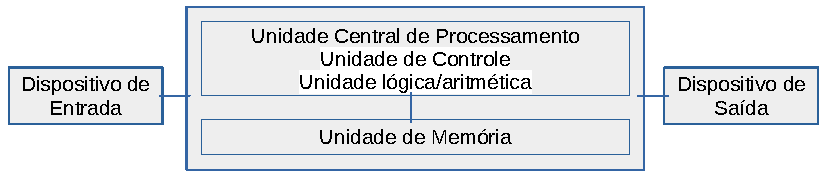
\includegraphics[width=\textwidth]{./cap_lingua/dados/fig_arqVonNeumann/main}
  \caption[Arquitetura de von Neumann]{Arquitetura de computador de von Neumann.}
  \label{cap_lim_sec_computador:fig:arqVonNeumann}
\end{figure}

Os computadores que comumente utilizamos seguem a arquitetura de John von Neumann\footnote{John von Neumann, 1903 - 1957, matemático húngaro, naturalizado estadunidense. Fonte: \href{https://pt.wikipedia.org/wiki/John_von_Neumann}{Wikipédia}.}, que consiste em dispositivo(s) de entrada de dados, unidade(s) de processamento, unidade(s) de memória e dispositivo(s) de saída de dados (Figura~\ref{cap_lim_sec_computador:fig:arqVonNeumann}).

\begin{itemize}
\item \hl{\emph{Dispositivos de entrada e saída}}

  São elementos do computador que permitem a comunicação humana (usuária(o)) com a máquina.

  \begin{itemize}
  \item \hl{\emph{Dispositivos de entrada}}

    São elementos que permitem o fluxo de informação da(o) usuária(o) para a máquina. Exemplos são: teclado, mouse/painel tátil, microfone, etc.

  \item \hl{\emph{Dispositivos de saída}}

    São elementos que permitem o fluxo de informação da máquina para a(o) usuária(o). Exemplos são: monitor/tela, alto-falantes, luzes espia, etc.
  \end{itemize}

\item \hl{\emph{Unidade central de processamento}}

  A \emph{CPU} (do inglês, {\it Central Processing Unit}) é o elemento de processa as informações e é composta de \emph{unidade de controle}, \emph{unidade lógica e aritmética} e de \emph{memória cache}.

  \begin{itemize}
  \item \hl{\emph{Unidade de controle}}

    Coordena as execuções do processador: busca e decodifica instruções, lê e escreve no {\it cache} e controla o fluxo de dados.

  \item \hl{\emph{Unidade lógica/aritmética}}

    Executa as instruções operações lógicas e aritméticas, por exemplo: executar a adição, multiplicação, testar se dois objetos são iguais, etc.

  \item \hl{\emph{Memória cache}}

    Memória interna da CPU muito mais rápida que as memórias RAM e dispositivos e armazenamento HDD/SSD. É um dispositivo de memória de pequena capacidade e é utilizada como memória de curto prazo e diretamente acessada.
  \end{itemize}

\item \hl{\emph{Unidades de memória}}

  As unidades de memória são elementos que permitem o armazenamento de dados/objetos. Como memória principal tem-se a \emph{ROM} (do inglês, {\it Read Only Memory}) e a \emph{RAM} (do inglês, {\it Random Access Memory}) e como memória de massa/secundária tem-se HDD, SSD, entre outras.

\item \hl{\emph{Memória ROM}}

  A memória ROM é utilizada para armazenamento de dados/objetos necessários para dar início ao funcionamento do computador. Por exemplo, é onde a BIOS (dos inglês, {\it Basic Input/Output System}, Sistema Básico de Entrada e Saída) é armazenada. Ao ligarmos o computador este programa é iniciado e é responsável por fazer o gerenciamento inicial dos diversos dispositivos do computador e carregar o \emph{sistema operacional} (conjunto de programas cuja função é de gerenciar os recursos do computador e controlar a execução de programas).

\item \hl{\emph{Memória RAM}}

  Memória de acesso rápido utilizada para dados/objetos de uso frequente durante a execução de programas. É uma memória volátil, i.e. toda a informação guardada nela é perdida quando o computador é desligado.

\item \hl{\emph{Memória de massa/secundária}}

  Memória de massa ou secundária são usadas para armazenar dados/objetos por período longo. Normalmente, são dispositivos HDD ou SSD, os dados/objetos são guardados mesmo que o computador seja desligado e contém grande capacidade de armazenagem.   
\end{itemize}

\hl{Os \emph{software} são os elementos lógicos de um sistema computacional, são programas de computadores que contém as instruções que gerenciam o \emph{hardware} para a execução de tarefas específicas}, por exemplo, imprimir um texto, gravar áudio/vídeo, resolver um problema matemático, etc. Programar é o ato de criar programas de computadores.

\subsection{Linguagem de programação}

\hl{As informações fluem no computador codificadas como registros de {\it bits}}\footnote{Usualmente de tamanho $64$-{\it bits}.} (sequência de zeros ou uns). Há registros de instrução e de dados. Programar diretamente por registros é uma tarefa muito difícil, o que levou ao surgimento de linguagens de programação. \hl{Uma \emph{linguagem de programação}\footnote{Código de programação, código de máquina ou linguagem de máquina.} é um método padronizado para escrever instruções para execução de tarefas no computador}. As instruções escritas em uma linguagem são interpretadas e/ou compiladas por um software (interpretador ou compilador) da linguagem que decodifica as instruções em registros de instruções e dados, os quais são efetivamente executados na máquina.

Existem várias linguagens de programação disponíveis e elas são classificadas por diferentes características. Uma \emph{linguagem de baixo nível} (por exemplo, \href{https://pt.wikipedia.org/wiki/Linguagem_assembly}{Assembly}) é aquela que se restringe às instruções executadas diretamente pelo processador, enquanto que uma \emph{linguagem de alto nível} contém instruções mais complexas e abstratas. Estas contém sintaxe mais próxima da linguagem humana natural e permitem a manipulação de objetos mais abstratos. Exemplos de linguagens de alto nível são: \href{https://pt.wikipedia.org/wiki/BASIC}{Basic}, \href{https://pt.wikipedia.org/wiki/Java\_(linguagem\_de\_programa\%C3\%A7\%C3\%A3o)}{Java}, \href{https://pt.wikipedia.org/wiki/JavaScript}{Javascript}, \href{https://pt.wikipedia.org/wiki/MATLAB}{MATLAB}, \href{https://pt.wikipedia.org/wiki/PHP}{PHP}, \href{https://pt.wikipedia.org/wiki/R\_(linguagem_de_programa\%C3\%A7\%C3\%A3o)}{R}, \href{https://pt.wikipedia.org/wiki/C\%2B\%2B}{C/C++}, {\python}, etc.

\hl{Em geral, não existe uma melhor linguagem, cada uma tem suas características que podem ser mais ou menos adequadas conforme o programa que se deseja desenvolver}. Por exemplo, para um site de internet, linguagens como \href{https://pt.wikipedia.org/wiki/JavaScript}{Javascript} e \href{https://pt.wikipedia.org/wiki/PHP}{PHP} são bastante úteis, mas não no desenvolvimento de modelagem matemática e computacional. Nestes casos, \href{https://pt.wikipedia.org/wiki/C\%2B\%2B}{C/C++} é uma linguagem mais apropriada por conter várias estruturas de programação que facilitam a modelagem computacional de problemas científicos. Agora, \href{https://pt.wikipedia.org/wiki/R\_(linguagem_de_programa\%C3\%A7\%C3\%A3o)}{R} é uma linguagem de alto nível com diversos recursos dedicados às áreas de ciências de dados e estatística. Usualmente, utiliza-se mais de uma linguagem no desenvolvimento de programas mais avançados. A ideia é de explorar o melhor de cada linguagem na criação de programas eficientes na resolução dos problemas de interesse.

Nestas notas de aula, \hl{{\python}} é a linguagem escolhida para estudarmos algoritmos e programação. Trata-se de uma \hl{linguagem de alto nível, \emph{interpretada}, \emph{dinâmica} e \emph{mutiparadigma}}. Foi lançada por Guido van Rossum\footnote{Guido van Rossum, 1956-, matemático e programador de computadores holandês. Fonte: \href{https://pt.wikipedia.org/wiki/Guido\_van\_Rossum}{Wikipédia}.} em 1991 e, atualmente, é desenvolvida de forma comunitária, aberta e gerenciada pela ONG \href{https://pt.wikipedia.org/wiki/Python_Software_Foundation}{Python Software Foundation}. A linguagem foi projetada para priorizar a legibilidade do código. Parte da filosofia da linguagem é descrita pelo poema \href{https://pt.wikipedia.org/wiki/Zen_de_Python}{The Zen of Python}. Pode-se lê-lo pelo {\it easter egg} {\python}:
\begin{lstlisting}
  >>> import this
\end{lstlisting}

\begin{itemize}
\item \hl{\emph{Linguagem interpretada}}

  {\python} é uma linguagem interpretada. Isso significa que o \emph{código-fonte} escrito em linguagem {\python} é interpretado por um programa (interpretador {\python}). Ao executar-se um código, o interpretador lê uma linha do código, decodifica-a como registros para o processador que os executa. Executada uma linha, o interpretador segue para a próxima até o código ter sido completadamente executado.

\item \hl{\emph{Linguagem compilada}}

  Em uma linguagem compilada, como \href{https://pt.wikipedia.org/wiki/C\%2B\%2B}{C/C++}, há um programa chamado de \emph{compilador} (em inglês, {\it compiler}) e outro de \emph{ligador} (em inglês, {\it linker}). O primeiro, cria um programa-objeto a partir do código e o segundo gerencia sua ligação com eventuais bibliotecas computacionais que ele possa depender. O programa-objeto (também chamado de executável) pode então ser executado pela máquina.
\end{itemize}

Em geral, a execução de um programa compilado é mais rápida que a de um código interpretado. De forma simples, isso se deve ao fato de que nesse a interpretação é feita toda de uma vez e não precisa ser refeita na execução de cada linha de código, como no segundo caso. Por outro lado, a compilação de códigos-fonte grandes pode ser bastante demorada fazendo mais sentido quando ele é compilado uma vez e o programa-objeto executado várias vezes. Além disso, linguagens interpretadas podem usar bibliotecas de programas pré-compiladas. Com isso, pode-se alcançar um bom balanceamento entre tempo de desenvolvimento e de execução do código.

O interpretador {\python} também pode ser usado para compilar o código para um arquivo \emph{bytecode}, este é executado muito mais rápido do que o código-fonte em si, pois as interpretações necessárias já foram feitas. Mais adiante, vamos estudar isso de forma mais detalhada.

\begin{itemize}
\item \hl{\emph{Linguagem de tipagem dinâmica}}

  {\python} é uma linguagem de tipagem dinâmica. Nela, os dados não precisam ser explicitamente tipificados no código-fonte e o interpretador os tipifica com base em regras da própria linguagem. Ao executar operações com os dados, o interpretador pode alterar seus tipos de forma dinâmica.

\item \hl{\emph{Linguagem de tipagem estática}}

  \href{https://pt.wikipedia.org/wiki/C\%2B\%2B}{C/C++} é um exemplo de uma linguagem de tipagem estática. Em tais linguagens, os dados devem ser explicitamente tipificados no código-fonte com base nos tipos disponíveis. A retipificação pode ocorrer, mas precisa estar explicitamente definida no código.
\end{itemize}

Existem vários \emph{paradigmas de programação} e a \hl{linguagem {\python} é multiparadigma}, i.e. permite a utilização de mais de um no código-fonte. Exemplos de paradigmas de programação são: \emph{estruturada}, \emph{orientada a objetos}, \emph{orientada a eventos}, etc.. Na maior parte destas notas de aulas, vamos estudar algoritmos para linguagens de programação estruturada. Mais ao final, vamos introduzir aspectos de linguagens orientada a objetos. Estes são paradigmas de programação fundamentais e suas estruturas são importantes na programação com demais paradigmas disponíveis em programação de computadores.

\subsection{Instalação e execução}

\hl{{\python} é um \emph{software aberto}}\footnote{Consulte a licença de uso em \url{https://docs.python.org/3/license.html}.} e está disponível para vários sistemas operacionais ({\linux}, macOS, Windows, etc.) no seu site oficial
\begin{center}
  \url{https://www.python.org/}
\end{center}
Também, está disponível (gratuitamente) na loja de aplicativos dos sistemas operacionais mais usados. Esta costuma ser a forma mais fácil de instalá-lo na sua máquina, consulte a loja de seus sistema operacional. Ainda, há plataformas e IDEs\footnote{IDE, do inglês, {\it Integrated Development enviroment}, ambiente de desenvolvimento integrado} {\python} disponíveis, consulte, como por exemplo, \href{https://www.anaconda.com/}{Anaconda}.

A execução de um código {\python} pode ser feita de várias formas.

\begin{itemize}
\item \hl{\emph{Execução iterativa via terminal}}

  Em terminal {\python} pode-se executar instruções/comandos de forma iterativa. Por exemplo:
  \begin{lstlisting}
    >>> print('Olá, mundo!')
    Olá, mundo!
    >>> 
  \end{lstlisting}

  \hl{O símbolo }\lstinline+>>>+\hl{ denota o \emph{prompt de entrada}, onde uma instrução {\python} pode ser digitada}. Após digitar, o comando é executada teclando \lstinline+<ENTER>+. Caso o comando tenha alguma \hl{saída de dados}, como no caso acima, esta aparecerá, por padrão, \hl{no \emph{prompt de saída}}, logo abaixo a linha de comando executada. \hl{Um novo símbolo de prompt de entrada aparece ao término da execução anterior}.

\item \hl{\emph{Execução de um {\it script}}}

  Para códigos com várias linhas de instruções é mais adequado utilizar um aquivo de {\it script} {\python}. Usando-se um editor de texto ou um IDE ditam-se as linhas de comando em um arquivo \lstinline+.py+. Então, {\it script} pode ser executado em um terminal de seu sistema operacional utilizando-se o interpretador {\python}. Por exemplo, assumindo que o código for salvo do arquivo \lstinline+path_to_arq/arq.py+, pode-se executá-lo em um terminal do sistema com
  \begin{lstlisting}
    $ python3 path_to_arq/arq.py 
  \end{lstlisting}%$
  

  IDEs para {\python} fornecem uma ambiente integrado, contendo um campo para escrita do código e terminal {\python} integrado. Consulte, por exemplo, o IDE {\spyder}:
  \begin{center}
    \url{https://www.spyder-ide.org/}
  \end{center}

\item \hl{\emph{Execução em um \textit{notebook}}}

  {\it Notebooks} {\python} são uma boa alternativa para a execução de códigos em um ambiente colaborativo/educativo. Por exemplo, {\jupyter} é um notebook que roda em navegadores de internet. Sua estrutura e soluções também são encontradas em notebooks online (de uso gratuito limitado) como {\colab} e {\kaggle}.  
\end{itemize}

\subsection{Exercícios}

\begin{exer}
  Verifique qual a versão do sistema operacional que está utilizado em seu computador.
\end{exer}
\begin{resp}
  Dica: Em {\linux}, \lstinline+$ uname --all+ ou \lstinline+$ cat /etc/version+.
\end{resp}

\begin{exer}
  Verifique os seguintes elementos de seu computador:
  \begin{enumerate}[a)]
  \item CPUs
  \item Placa(s) gráfica(s)
  \item Memória RAM
  \item Armazenamento HDD/SSD.
  \end{enumerate}
\end{exer}
\begin{resp}
  Dica: Em {\linux}: \lstinline*$ lshw*%$
\end{resp}

\begin{exer}
  Verifique como entrar na \lstinline+BIOS+ de seu computador. Atenção! Não faça  e salve nenhuma alteração, caso não saiba o que está fazendo. Modificações na \lstinline+BIOS+ podem impedir que seu computador funcione normalmente, inclusive, impedir que você inicialize seu sistema operacional.
\end{exer}
\begin{resp}
  Dica: cada computador tem sua forma de acessar a \lstinline+BIOS+. Verifique o manual ou busque na internet pela marca e modelo de seu computador.
\end{resp}

\begin{exer}
  Instale {\python} no seu computador (caso ainda não tenha feito) e abra um terminal {\python}. Nele, escreva uma linha de comando que imprima no prompt de saída a frase ``Olá, meu Python!''.
\end{exer}
\begin{resp}
\begin{lstlisting}
>>> print('Olá, meu Python!')
Olá, meu Python!
>>> 
\end{lstlisting}
\end{resp}

\begin{exer}
  Instale o {\spyder} no seu computador (caso ainda não tenha feito) e use-o para escrever o seguinte {\it script}
\begin{lstlisting}
import math as m
print(f'Número pi = {m.pi}')
print(f'Número de Euler e = {m.e}')
\end{lstlisting}
  Também, execute o {\it script} diretamente em um terminal de seu sistema operacional.
\end{exer}

\begin{exer}
  Use um {\it notebook} {\python} para escrever e executar o código do exercício anterior.
\end{exer}
\begin{resp}
  Dica: use um notebook online {\colab}, {\kaggle} ou {\jupyter}.
\end{resp}

\section{Algoritmos e Programação}\label{cap_lingua_sec_algoprog}

\hl{\emph{Programar} é criar um programa} (um {\it software}) \hl{para ser executado em computador}. Para isso, escreve-se \hl{um código em uma linguagem computacional} (por exemplo, em {\python}), o qual é interpretado/compilado para gerar o programa final. \hl{Linguagens computacionais são técnicas, utilizam uma sintaxe simples, precisa e sem ambiguidades}. Ou seja, para criarmos um programa com um determinado objetivo, precisamos escrever um código computacional técnico, que siga a sintaxe da linguagem escolhida e sem ambiguidades.

\hl{Um \emph{algoritmo} pode ser definido uma sequencia ordenada e sem ambiguidade de passos para a resolução de um problema}.

\begin{ex}\label{cap_lingua_sec_algoprog:ex:areaTriang}
O cálculo da área de um triângulo de base e altura dadas por ser feito com o seguinte algoritmo:
\begin{enumerate}
\item Informe o valor da base $b$.
\item Informe o valor da altura $h$.
\item $\displaystyle a \leftarrow \frac{b\cdot h}{2}$.
\item Imprima o valor de $a$.
\end{enumerate}

\hl{Algoritmos para a programação são pensados para serem facilmente transformados em códigos computacionais}. Por exemplo, o algoritmo acima pode ser escrito em {\python} como segue:
\begin{lstlisting}
b = float(input('Informe o valor da base.\n'))
h = float(input('Informe o valor da altura.\n'))
# cálculo da área
a = b*h/2
print(f'Área = {a}')
\end{lstlisting}
\end{ex}

Para criar um programa para resolver um dado problema, começamos desenvolvendo um algoritmo para resolvê-lo, este algoritmo é implementado na linguagem computacional escolhida, a qual gera o programa final. Aqui, o passo mais difícil costuma ser o desenvolvimento do algoritmo. Precisamos pensar em como podemos resolver o problema de interesse em uma sequência de passos ordenada e sem ambiguidades para que possamos implementá-los em computador.

\hl{Um algoritmo deve ter as seguintes propriedades}:
\begin{itemize}
\item \hl{Cada passo deve estar bem definido}, i.e. não pode conter ambiguidades.
\item \hl{Cada passo deve contribuir de forma efetiva na solução do problema}.
\item \hl{Deve ter número finito de passos} que podem ser \hl{computados em um tempo finito}.
\end{itemize}

\begin{obs}
  A primeira pessoa a publicar um algoritmo para programação foi Augusta Ada King\footnote{Augusta Ada King, 1815 - 1852, matemática e escritora inglesa. Fonte: \href{https://pt.wikipedia.org/wiki/Ada_Lovelace}{Wikipédia}.}. O algoritmo foi criado para computar os \href{https://pt.wikipedia.org/wiki/N\%C3\%BAmeros\_de\_Bernoulli}{números de Bernoulli}\footnote{Jacob Bernoulli, 1655-1705, matemático suíço. Fonte: \href{https://pt.wikipedia.org/wiki/Jakob_Bernoulli}{Wikipédia}.}.
\end{obs}


\subsection{Fluxograma}

\hl{Fluxograma é uma representação gráfica de um algoritmo}. Entre outras, usam-se as seguintes formas para representar tipos de ações a serem executadas:
\begin{itemize}
\item \hl{\emph{Terminal}: início ou final do algoritmo}.
  \begin{center}
    
\includegraphics{./cap_lingua/dados/fig_fluxograma/terminal}
  \end{center}  
\item \hl{\emph{Linha de fluxo}: direciona para a próxima execução}.
  \begin{center}
    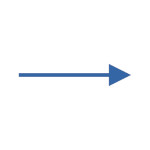
\includegraphics{./cap_lingua/dados/fig_fluxograma/linha}
  \end{center}
\item \hl{\emph{Entrada}: leitura de informação/dados}.
  \begin{center}
    
\includegraphics{./cap_lingua/dados/fig_fluxograma/entrada}
  \end{center}  
\item \hl{\emph{Processo}: ação a ser executada}.
  \begin{center}
    
\includegraphics{./cap_lingua/dados/fig_fluxograma/processo}
  \end{center}
\item \hl{\emph{Decisão}: ramificação do processamento baseada em uma condição}.
  \begin{center}
    
\includegraphics{./cap_lingua/dados/fig_fluxograma/decisao}
  \end{center}
\item \hl{\emph{Saída}: impressão de informação/dados}.
  \begin{center}
    
\includegraphics{./cap_lingua/dados/fig_fluxograma/saida}
\end{center}
\end{itemize}

\begin{ex}\label{cap_lingua_sec_algoprog:ex:metHeron}
  O \href{https://en.wikipedia.org/wiki/Methods_of_computing_square_roots#Heron's_method}{método de Heron}\footnote{Heron de Alexandria, 10 - 80, matemático e inventor grego. Fonte: \href{https://pt.wikipedia.org/wiki/Heron\_de\_Alexandria}{Wikipédia}.} é um algoritmo para o cálculo aproximado da raiz quadrada de um dado número $x$, i.e. $\sqrt{x}$. Consiste na iteração
  \begin{align}
    s^{(0)} &= \text{approx. inicial},\\
    s^{(i+1)} &= \frac{1}{2}\left(s^{(i)} + \frac{x}{s^{(i)}}\right),
  \end{align}
  para $i=0,1,2,\ldots,n$, onde $n$ é o número de iterações calculadas.

  Na sequência, temos um algoritmo e seus fluxograma e código {\python} para computar a quarta aproximação de $\sqrt{x}$, assumindo $s^{(0)} = x/2$ como aproximação inicial.

  \begin{itemize}
  \item \emph{Algoritmo}
    \begin{enumerate}
    \item Entre o valor de $x$.
    \item Se $x\geq 0$, faça:
      \begin{enumerate}
      \item $s \leftarrow x/2$
      \item Para $i = 0,1,2,3$, faça:
        \begin{enumerate}
        \item $s \leftarrow (s + x/s)/2$.
        \end{enumerate}
      \item Imprime o valor de $s$.
      \end{enumerate}
    \item Senão, faça:
      \begin{enumerate}
      \item Imprime mensagem ``Não existe!''.
      \end{enumerate}
    \end{enumerate}

  \item \emph{Fluxograma}

    \begin{center}
      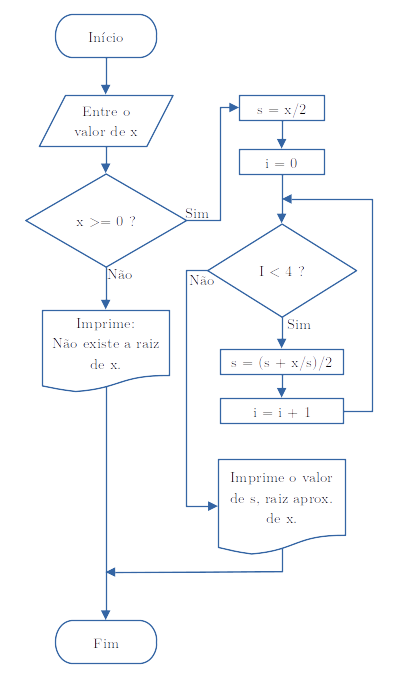
\includegraphics{./cap_lingua/dados/fig_fluxograma/fig}
    \end{center}

  \item \emph{Código {\python}}

\begin{lstlisting}[caption=metHeron.py,label=cap_lingua_sec_algoprog:cod:metHeron]
x = float(input('Entre com o valor de x: '))
if (x >= 0.):
    s = x/2
    for i in range(4):
        s = (s + x/s)/2
    print(f'Raiz aprox. de x = {s}')
else:
    print(f'Não existe!')
\end{lstlisting}
  \end{itemize}

  O algoritmo apresentado acima tem um {\it bug} (um erro)! Consulte o Exercício~\ref{cap_lingua_sec_algoprog:exer:bugHeron}.
\end{ex}

\hl{Algoritmos escritos em uma forma próxima de uma linguagem computacional} são, também, chamados de \hl{\emph{pseudocódigos}}. Na prática, pseudocódigos e fluxogramas são usados para apresentar uma forma mais geral e menos detalhada de um algoritmo. Usualmente, sua forma detalhada é escrita diretamente em uma linguagem computacional escolhida.

\subsection{Exercícios}

\begin{exer}
  Escreva um algoritmo/pseudocódigo e um fluxograma correspondente para o calcular a média aritmética entre dois números $x$ e $y$ dados. Como desafio, tente escrever um código {\python} baseado em seu algoritmo.
\end{exer}

\begin{exer}
  Escreva um algoritmo/pseudocódigo e um fluxograma correspondente para o calcular a área de um quadrado de lado $l$ dado. Como desafio, tente escrever um código {\python} baseado em seu algoritmo.
\end{exer}

\begin{exer}
  Escreva um algoritmo/pseudocódigo e um fluxograma correspondente para o calcular a área de um retângulo de lados $a, b$ dados. Como desafio, tente escrever um código {\python} baseado em seu algoritmo.
\end{exer}

\begin{exer}
  Escreva um algoritmo/pseudocódigo e um fluxograma correspondente para o calcular triângulo retângulo de hipotenusa $h$ e um dos lados $l$ dados. Como desafio, tente escrever um código {\python} baseado em seu algoritmo.
\end{exer}

\begin{exer}
  Escreva um algoritmo/pseudocódigo e um fluxograma correspondente para o calcular o zero de uma função afim
  \begin{equation}
    f(x) = ax + b
  \end{equation}
  dados, os coeficientes $a$ e $b$. Como desafio, tente escrever um código {\python} baseado em seu algoritmo.
\end{exer}

\begin{exer}
  Escreva um algoritmo/pseudocódigo e um fluxograma correspondente para o calcular as raízes reais de um polinômio quadráticos
  \begin{equation}
    p(x) = ax^2 + bx + c
  \end{equation}
  dados, os coeficientes $a$, $b$ e $c$. Como desafio, tente escrever um código {\python} baseado em seu algoritmo.
\end{exer}

\begin{exer}
  A \href{https://pt.wikipedia.org/wiki/S%C3%A9rie_harm%C3%B3nica_(matem%C3%A1tica)}{Série Harmônica} é defina por
  \begin{equation}
    \sum_{k=1}^\infty\frac{1}{k} := \frac{1}{1} + \frac{1}{2} + \frac{1}{3} + \cdots
  \end{equation}
  Escreva um algoritmo/pseudocódigo e um fluxograma corresponde para calcular o valor da série harmônica truncada em $k=n$, com $n$ dado. Ou seja, dado $n$, o objetivo é calcular
  \begin{equation}
    \sum_{k=1}^n\frac{1}{k} := \frac{1}{1} + \frac{1}{2} + \cdots + \frac{1}{n}.
  \end{equation}
\end{exer}

\begin{exer}
  O \href{https://pt.wikipedia.org/wiki/E_(constante_matem%C3%A1tica)}{número de Euler}{\euler} pode ser definido pela série
  \begin{align}
    e &:= \sum_{k=0}^\infty\frac{1}{k!}\\
      &= \frac{1}{0!} + \frac{1}{1!} + \frac{1}{2!} + \frac{1}{3!} + \frac{1}{4!} + \cdots
  \end{align}
  Escreva um algoritmo/pseudocódigo e um fluxograma corresponde para calcular o valor aproximado de $e$ dado pelo truncamento da série em $k=4$, i.e. o objetivo é de calcular
  \begin{align}
    e &\approx \sum_{k=0}^4\frac{1}{k!}\\
      &= \frac{1}{0!} + \frac{1}{1!} + \frac{1}{2!} + \frac{1}{3!} + \frac{1}{4!}\\
      &= \frac{1}{1} + \frac{1}{1} + \frac{1}{1\cdot 2} + \frac{1}{1\cdot 2\cdot 3} + \frac{1}{1\cdot 2\cdot 3\cdot 4}.
  \end{align}
\end{exer}

\begin{exer}\label{cap_lingua_sec_algoprog:exer:bugHeron}
  O algoritmo construído no Exemplo~\ref{cap_lingua_sec_algoprog:ex:metHeron} tem um {\it bug} (um erro). Identifique o {\it bug} e proponha uma nova versão para corrigir o problema. Então, apresente o fluxograma da nova versão do algoritmos. Como desafio, busque implementá-lo em {\python}. 
\end{exer}
\begin{resp}
  Dica: o {\it bug} ocorre quando $x = 0$.
\end{resp}

\section{Dados}\label{cap_lingua_sec_dados}

Informação é resultante do processamento, manipulação e organização de \emph{dados} (altura, quantidade, volume, intensidade, densidade, etc.). \hl{Programas de computadores processam, manipulam e organizam \emph{dados computacionais}}. Os dados computacionais são representações em máquina de dados ``reais''. De certa forma, todo dado é uma abstração e, para ser utilizado em um programa de computador, precisa ser representado em máquina.

\hl{Cada dado manipulado em um programa é identificado por um \emph{nome}}, chamado de \hl{\emph{identificador}}. Podem ser variáveis, constantes, funções/métodos, entre outros.
\begin{itemize}
\item \hl{\emph{Variável}}

  Objetos de um programa que armazenam dados que podem mudar de valor durante a sua execução.

\item \hl{\emph{Constantes}}

  Objetos de um programa que não mudam de valor durante a sua execução.

\item \hl{\emph{Funções e métodos}}

  Subprogramas definidos e executados em um programa.
\end{itemize}

\subsection{Identificadores}

\hl{Um identificador é um nome atribuído para a identificação inequívoca de dados que são manipulados em um programa}.

\begin{ex}\label{cap_lingua_sec_dados:ex:reta}
  Vamos desenvolver um programa que computa o ponto de interseção da reta de equação
  \begin{equation}
    y = ax + b
  \end{equation}
  com o eixo $x$ (consulte a Figura~\ref{cap_lingua_sec_dados:fig:ex_reta}).

  \begin{figure}[H]
    \centering
    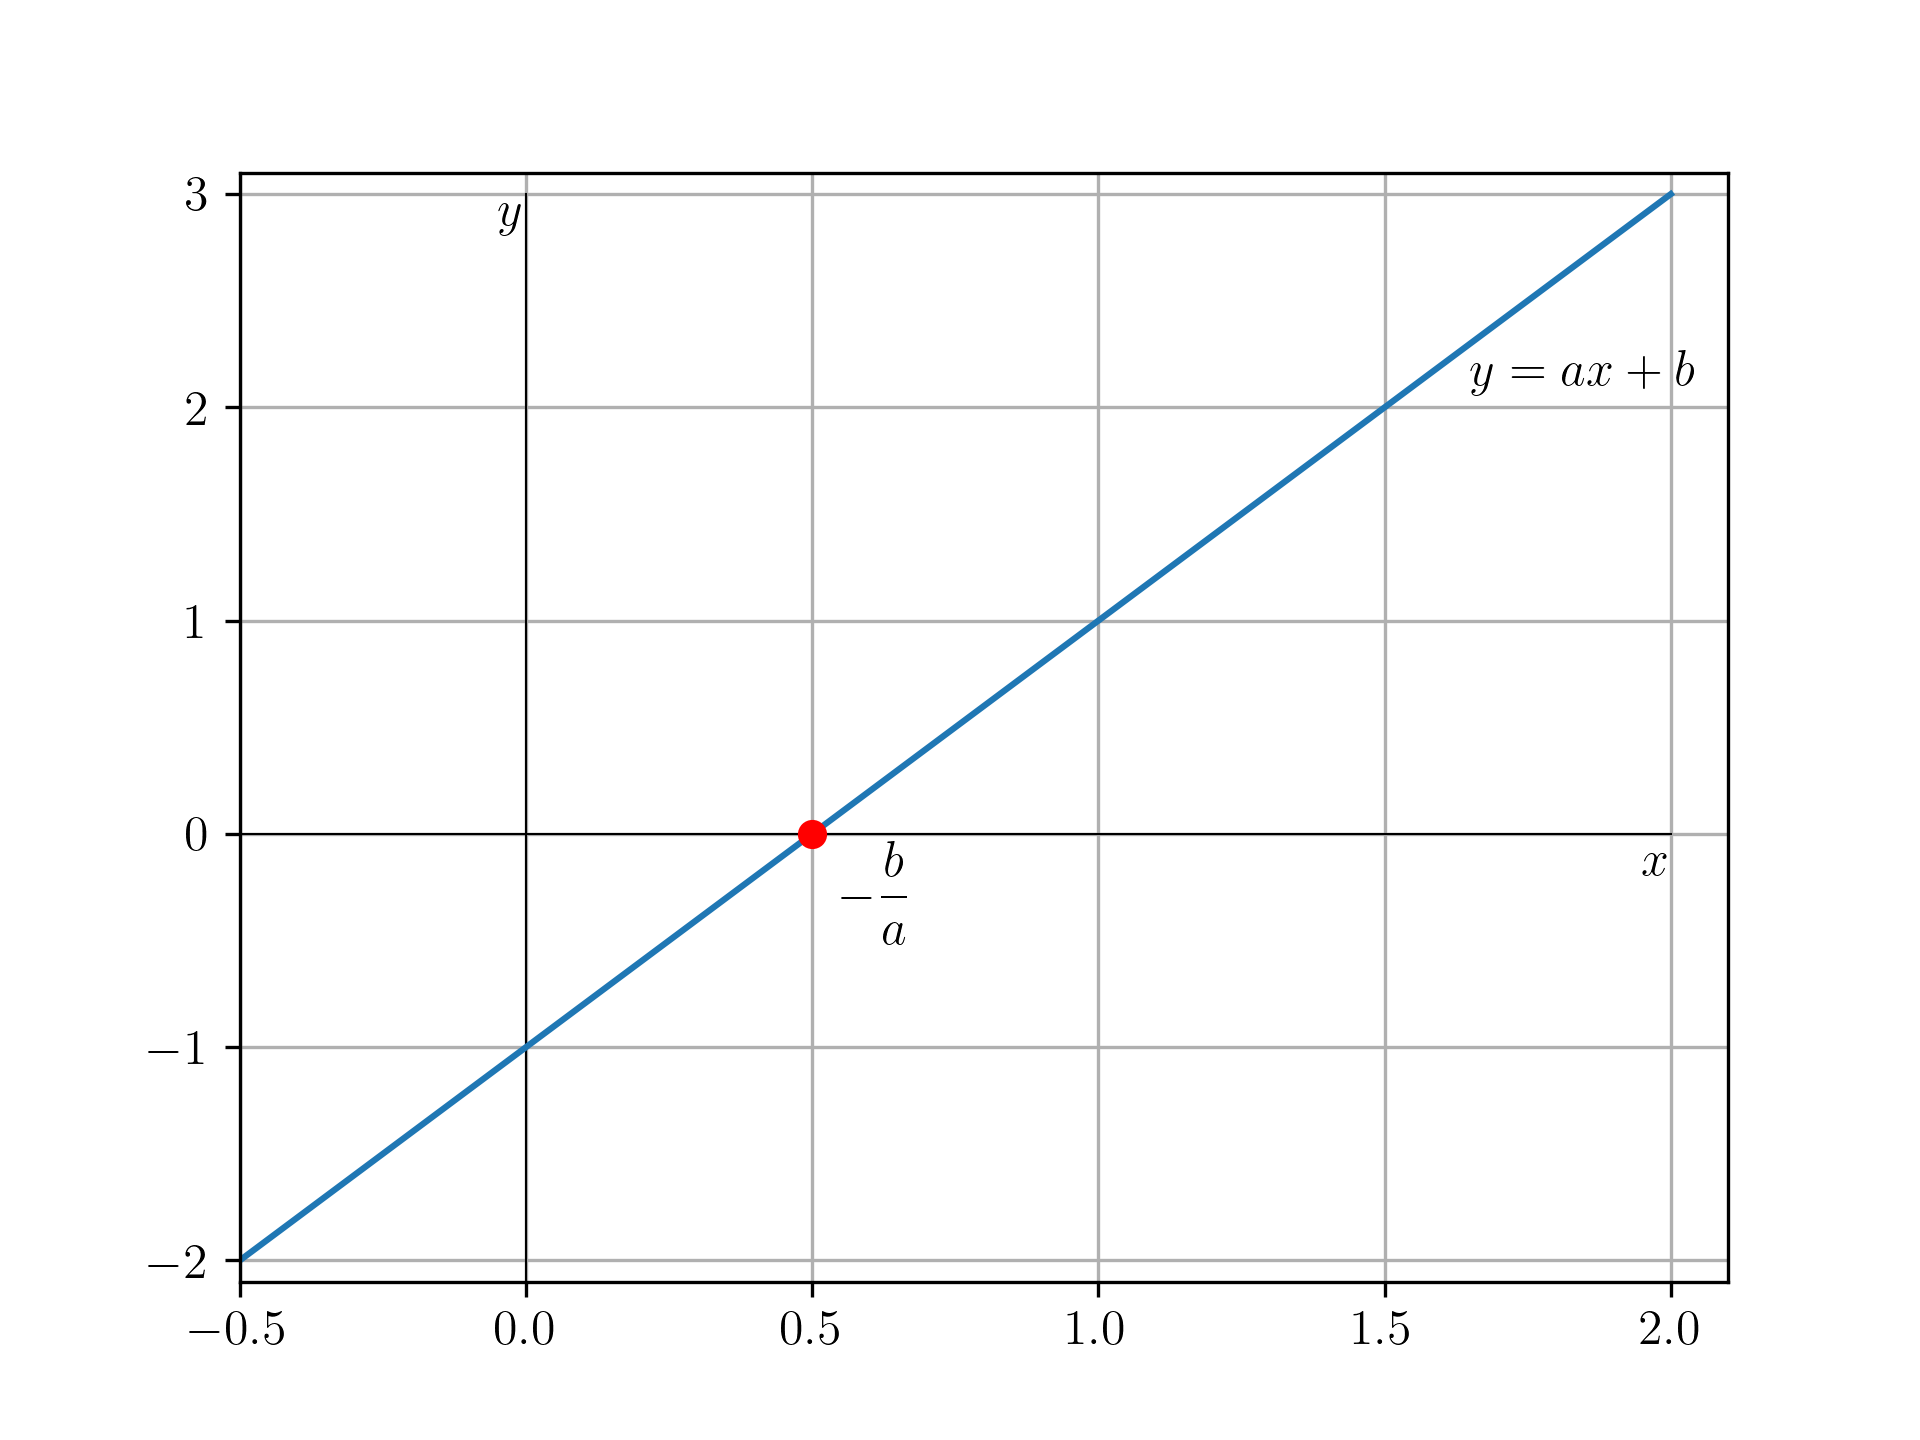
\includegraphics[width=\textwidth]{./cap_lingua/dados/fig_ex_reta/fig}
    \caption{Esboço da reta de equação $y = ax + b$, com $a=2$ e $b=-1$.}
    \label{cap_lingua_sec_dados:fig:ex_reta}
  \end{figure}

  O ponto $x$ em que a reta intercepta o eixo das abscissas é
  \begin{equation}
    x = -\frac{b}{a}
  \end{equation}
  Assumindo que $a=2$ e $b=-1$, segue um algoritmo para a computação.
  \begin{enumerate}
  \item Atribui o valor do \emph{coeficiente angular}:
    \begin{equation}
      a\leftarrow 2.
    \end{equation}
  \item Atribui o valor do \emph{coeficiente linear}:
    \begin{equation}
      b\leftarrow -1.
    \end{equation}
  \item Computa e armazena o valor do \emph{ponto de interseção com o eixo $x$}:
    \begin{equation}
      x \leftarrow -\frac{b}{a}.
    \end{equation}
  \item Imprime o valor de $x$.
  \end{enumerate}

  No algoritmo acima, os identificados utilizados foram: $a$ para o \emph{coeficiente angular}, $b$ para o \emph{coeficiente linear} e $x$ para o \emph{ponto de interseção com o eixo x}.
\end{ex}


\hl{Em {\python}, os identificadores são sensíveis a letras maiúsculas e minúsculas (em inglês, \textit{case sensitive})}, i.e. o identificador \lstinline+nome+ é diferente dos \lstinline+Nome+, \lstinline+NoMe+ e \lstinline+NOME+. Por exemplo:
\begin{lstlisting}
>>> a = 7
>>> print(A)
Traceback (most recent call last):
  File "<stdin>", line 1, in <module>
NameError: name 'A' is not defined. Did you mean: 'a'?
\end{lstlisting}

\hl{Para melhorar a legibilidade de seus códigos, recomenda-se utilizar identificadores com nomes compostos} que ajudem a lembrar o significado do dado a que se referem. No exemplo acima (Exemplo~\ref{cap_lingua_sec_dados:ex:reta}), $a$ representa o \emph{coeficiente angular} da reta e um identificar apropriado seria \lstinline+coefAngular+ ou \lstinline+coef_angular+.

\hl{Identificadores não podem conter caracteres especiais} (\lstinline+*+, \lstinline+&+, \lstinline+%+,
\lstinline+ç+, acentuações, etc.), \hl{espaços em branco e começar com número}. As seguintes convenções para identificadores com nomes compostos são recomendadas:
\begin{itemize}
\item \hl{\emph{lowerCamelCase}: {\lstinline+nomeComposto+}}
\item \hl{\emph{UpperCamelCase}: {\lstinline+NomeComposto+}}
\item \hl{\emph{snake}: {\lstinline+nome_composto+}}
\end{itemize}

Alguns identificadores são palavras reservadas pela linguagem, pois representam dados pré-definidos nela. Veja a lista de identificadores reservados em \href{https://docs.python.org/3/reference/lexical_analysis.html#keywords}{Python Docs: Lexical Analysis: Keywords}.

\begin{ex}
  O algoritmo construído no Exemplo~\ref{cap_lingua_sec_dados:ex:reta} pode ser implementado como segue:
\begin{lstlisting}
coefAngular = 2
coefLinear = -1
intercepEixoX = -coefLinear/coefAngular
print(intercepEixoX)
\end{lstlisting}
\end{ex}

\subsection{Alocação de dados}

Como estudamos acima, \hl{alocamos e referenciamos dados na memória do computador usando identificadores}. Em {\python}, ao executarmos a instrução
\begin{lstlisting}
>>> x = 1
\end{lstlisting}
estamos criando um \emph{objeto} na memória com valor $1$ e \lstinline+x+ é uma referência para este dado alocado na memória. Pode-se imaginar a memória computacional como um sequência de caixinhas, de forma que \lstinline+x+ será a identificação da caixinha onde o valor $1$ foi alocado.

\begin{center}
  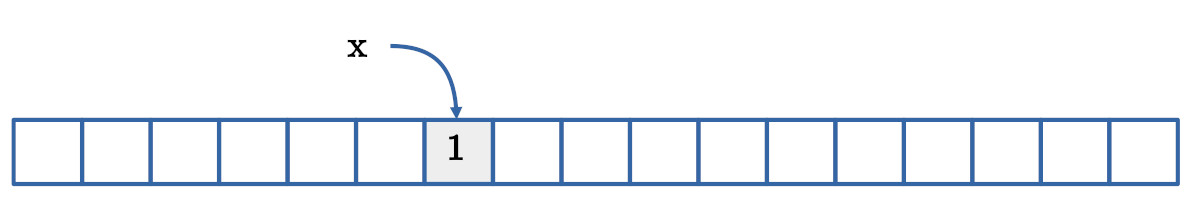
\includegraphics[width=\textwidth]{./cap_lingua/dados/fig_aloc_mem/xRecebe1}
\end{center}

Agora, quando executamos a instrução
\begin{lstlisting}
>>> y = x 
\end{lstlisting}
o identificador \lstinline+y+ passa a referenciar o mesmo local de memória de \lstinline+x+.

\begin{center}
  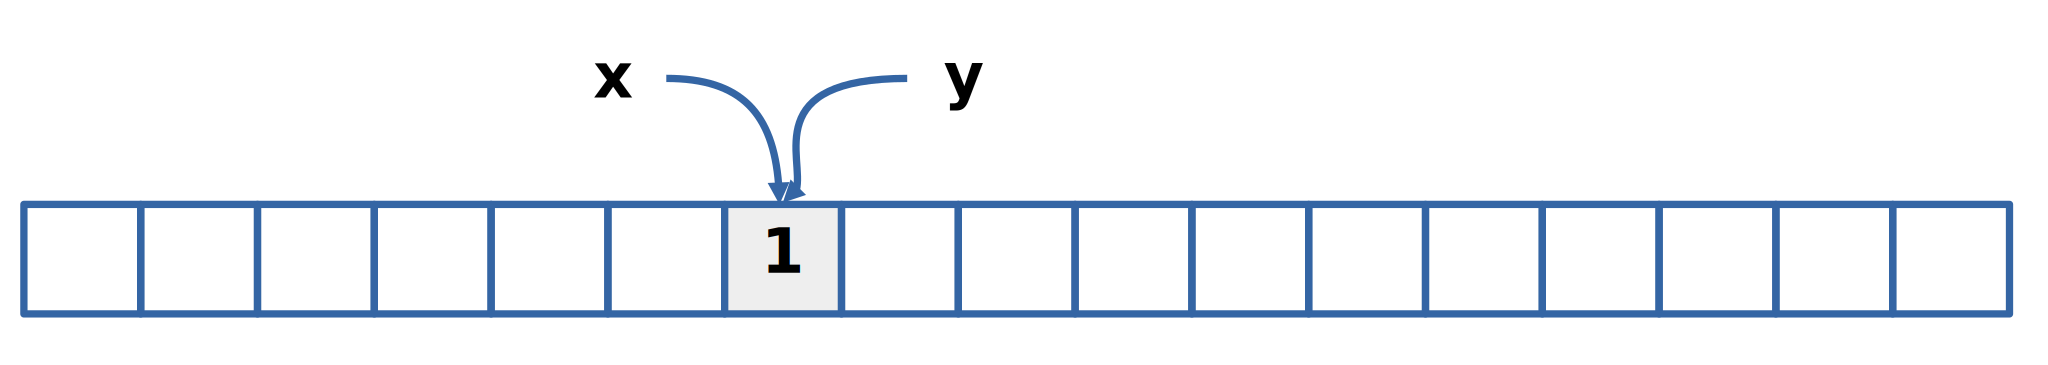
\includegraphics[width=\textwidth]{./cap_lingua/dados/fig_aloc_mem/yRecebex}
\end{center}

Na sequência, se atribuirmos um novo valor para \lstinline+x+
\begin{lstlisting}
>>> x = 2
\end{lstlisting}
este será alocado em um novo local na memória e \lstinline+x+ passa a referenciar este novo local.

\begin{center}
  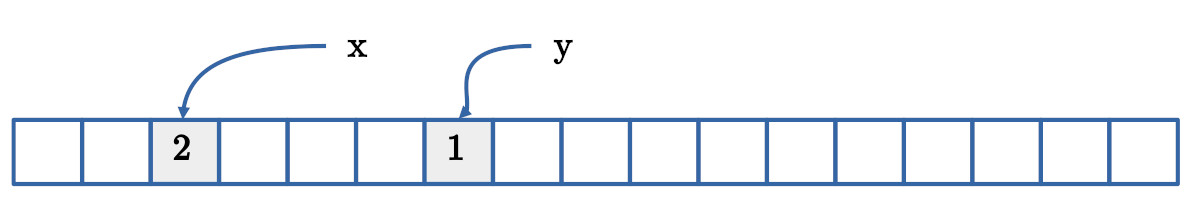
\includegraphics[width=\textwidth]{./cap_lingua/dados/fig_aloc_mem/xRecebe2}
\end{center}

Ainda, se atribuirmos um novo valor para \lstinline+y+
\begin{lstlisting}
>>> y = 3
\end{lstlisting}
este será alocado em um novo local na memória e \lstinline+y+ passa a referenciar este novo local. O local de memória antigo, em que o valor $2$ está alocado, passa a ficar novamente disponível para o sistema operacional.

\begin{center}
  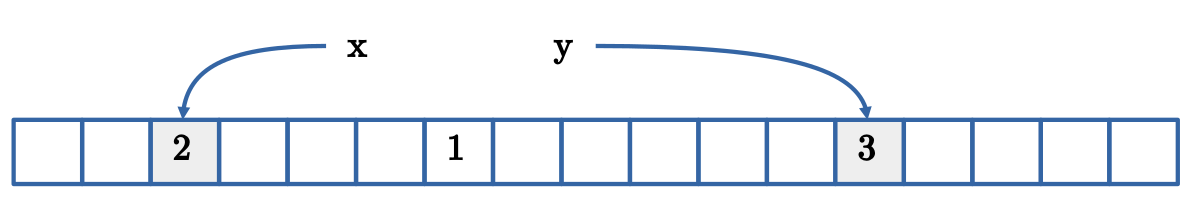
\includegraphics[width=\textwidth]{./cap_lingua/dados/fig_aloc_mem/yRecebe3}
\end{center}

\begin{obs}
  O método {\python} \href{https://docs.python.org/3/library/functions.html?highlight=id#id}{\lstinline+id+} retorna a identidade (endereço da caixinha) de um objeto. Essa identidade deve ser única e constante para cada objeto.
\begin{lstlisting}
>>> x = 1
>>> id(x)
139779845161200
>>> y = x
>>> id(y)
139779845161200
>>> x = 2
>>> id(x)
139779845161232
>>> id(y)
139779845161200
>>> y = 3
>>> id(y)
139779845161264
\end{lstlisting}
\end{obs}

\begin{ex}\normalfont{(\hl{Troca de Variáveis/Identificadores}.)}\label{cap_lingua_sec_dados:ex:trocaVar}
Em várias situações, faz-se necessário permutar dados entre dois identificadores. Sejam
\begin{lstlisting}
x = 1
y = 2
\end{lstlisting}
Agora, queremos permutar os dados, ou seja, queremos que \lstinline+y+ tenha o valor $1$ e \lstinline+x+ o valor $2$. Podemos fazer isso utilizando uma variável auxiliar (em inglês, {\it buffer}).
\begin{lstlisting}
z = x
x = y
y = z
\end{lstlisting}
Verifique!
\end{ex}

\subsection{Exercícios}

\begin{exer}
  Proponha identificadores adequados à linguagem {\python} baseados nos seguintes nomes:
  \begin{enumerate}[a)]
  \item Área
  \item Perímetro do quadrado
  \item Cateto+Cateto
  \item Número de elementos do conjunto A
  \item 77 lados
  \item $f(x)$
  \item $x^2$
  \item $13x$
  \end{enumerate}
\end{exer}
\begin{resp}
  a) \lstinline+area+; b) \lstinline+perimetroQuad+; c) \lstinline+somaCatetos+; d) \lstinline+numElemA+; e) \lstinline+lados77+; f) \lstinline+fx+; g) \lstinline+x2+; h) \lstinline+xv13+
\end{resp}

\begin{exer}
  No Exemplo~\ref{cap_lingua_sec_algoprog:ex:areaTriang}, apresentamos um código {\python} para o cálculo da área de um triângulo. Reescreva o código trocando seus identificadores por nomes mais adequados.
\end{exer}
\begin{resp}
\begin{lstlisting}
base = float(input('Informe o valor da base.\n'))
altura = float(input('Informe o valor da altura.\n'))
# cálculo da área
area = base * altura /2
print(f'Área = {area}')
\end{lstlisting}
\end{resp}

\begin{exer}
  O seguinte código {\python} tem um erro:
\begin{lstlisting}
x = 1
y = X + 1
\end{lstlisting}
  Identifique-o e apresente uma nova versão código corrigido.
\end{exer}
\begin{resp}
  Erro: variável $X$ não foi definida.
\begin{lstlisting}
x = 1
y = x + 1
\end{lstlisting}
\end{resp}

\begin{exer}
  Faça uma representação gráfica da alocação de memória que ocorre para cada uma das instruções {\python} do Exemplo~\ref{cap_lingua_sec_dados:ex:trocaVar} na troca de variáveis. Ou seja, para a seguinte sequência de instruções:
\begin{lstlisting}
x = 1
y = 2
z = x
x = y
y = z
\end{lstlisting}
\end{exer}

\begin{exer}
  No Exemplo~\ref{cap_lingua_sec_dados:ex:trocaVar} fazemos a permutação entre as variáveis \lstinline+x+ e \lstinline+y+ usando um {\it buffer} \lstinline+z+ para guardar o valor de \lstinline+x+. Se, ao contrário, usarmos o {\it buffer} para guardar o valor de \lstinline+y+, como fica o código de permutação entre as variáveis?
\end{exer}
\begin{resp}
  \begin{lstlisting}
    x = 1
    y = 2
    z = y
    y = x
    x = z
    print(x, y)
    2 1
  \end{lstlisting}
\end{resp}

\section{Dados Numéricos e Operações}\label{cap_lingua_sec_numop}

Números são tipos de dados comumente manipulados \hl{em programas de computador}. \hl{Números inteiros e não inteiros são tratados de forma diferente}. Mas, antes de discorrermos sobre essas diferenças, vamos estudar operadores numéricos básicos.

\subsubsection{Operações Numéricas Básicas}

As seguintes operações numéricas estão disponíveis na linguagem {\python}:
\begin{itemize}
\item \hl{{\lstinline*+*} \emph{ : adição}}
\begin{lstlisting}
>>> 1 + 2
3
\end{lstlisting}
\item \hl{{\lstinline+-+} \emph{ : subtração}}
\begin{lstlisting}
>>> 1 - 2
-1
\end{lstlisting}
\item \hl{{\lstinline+*+} \emph{ : multiplicação}}
\begin{lstlisting}
>>> 2*3
6
\end{lstlisting}
\item \hl{{\lstinline+/+} \emph{ : divisão}}
\begin{lstlisting}
>>> 5/2
2.5
\end{lstlisting}
\item \hl{{\lstinline+//+} \emph{ : divisão inteira}}
\begin{lstlisting}
>>> 5//2
2
\end{lstlisting}
\item \hl{\texttt{\%} \emph{ : resto da divisão}}
\begin{lstlisting}
>>> 5 % 2
1
\end{lstlisting}
\end{itemize}

A \hl{\emph{ordem de precedência das operações}} deve ser observada em {\python}. \hl{Uma expressão é executada da esquerda para a direita, mas os operadores tem a seguinte precedência}\footnote{Consulte a lista completa de operadores e suas precedências em \href{https://docs.python.org/3/reference/expressions.html\#operator-precedence}{Python Docs: Expressions: Operator precedence}.}:
\begin{enumerate}
\item \lstinline+**+
\item lstinline*-x* \emph{: oposto de $x$}
\item \lstinline+*, /, //, %+
\item \lstinline*+, -*
\end{enumerate}
\hl{Utilizamos parênteses para impor uma precedência diferente}, i.e. expressões entre parênteses \lstinline+()+ são executadas antes das demais.

\begin{ex}
  Estudamos a seguinte computação:
\begin{lstlisting}
>>> 2+8*3/2**2-1
7.0
\end{lstlisting}

  Uma pessoa desavisada poderia pensar que o resultado está errado, pois
  \begin{gather}
    2+8 = 10,\\
    10 \cdot 3 = 30,\\
    30 \div 2 = 15,\\
    15^2 = 225,\\
    225 - 1 = 224.
  \end{gather}
  Ou seja, o resultado não deveria ser $224$? Não, em {\python}, a operação de potenciação \lstinline+**+ tem a maior precedência, depois vem as de multiplicação \lstinline+*+ e divisão \lstinline+/+ (com a mesma precedência, sendo que a mais a esquerda é executada primeiro) e, por fim, vem as de adição \lstinline*+* e subtração \lstinline+-+ (também com a mesma precedência entre si). Ou seja, a instrução acima é computada na seguinte ordem:
  \begin{gather}
    2^2 = 4,\\
    8\cdot 3 = 24,\\
    24\div 4 = 6,\\
    2 + 6 = 8,\\
    8 - 1 = 7.
  \end{gather}

  Para impormos um ordem diferente de precedência, usamos parêntese. No caso acima, escrevemos
\begin{lstlisting}
>>> ((2 + 8)*3/2)**2 - 1
224.0
\end{lstlisting}
\end{ex}

O uso de espaços entre os operandos,em geral, é arbitrário, mas conforme utilizados podem dificultar a legibilidade do código.

\begin{ex}
  Consideramos a seguinte expressão
\begin{lstlisting}
>>> 2 *- 3 + 2
-4
\end{lstlisting}
  Essa expressão é computada na seguinte ordem:
  \begin{gather}
    -~3 = -3\\
    2\cdot(-3) = -6\\
    -6 + 2 = -4
  \end{gather}
  Observamos que ela seria melhor escrita da seguinte forma:
\begin{lstlisting}
>>> 2*-3 + 2
-4
\end{lstlisting}
\end{ex}

\subsection{Números Inteiros}

\hl{Em {\python}, números inteiros são alocados por registros com um número arbitrário de {\it bits}}. Com isso, os maior e menor números inteiros que podem ser alocados dependem da capacidade de memória da máquina. \hl{Quanto maior ou menor o número inteiro, mais {\it bits} são necessários para alocá-lo}.

\begin{ex}
  O método {\python} \href{https://docs.python.org/3/library/sys.html#sys.getsizeof}{\lstinline+sys.getsizeof()+} retorna o tamanho de um objeto medido em {\it bytes} \hl{($1~\textit{byte} = 8~\textit{bits}$)}.
\begin{lstlisting}
>>> import sys
>>> sys.getsizeof(0)
24
>>> sys.getsizeof(1)
28
>>> sys.getsizeof(100)
28
>>> sys.getsizeof(10**9)
28
>>> sys.getsizeof(10**10)
32
>>> sys.getsizeof(10**100) #googol
72
\end{lstlisting}

  O número \href{https://en.wikipedia.org/wiki/Googol}{googol} $10^{100}$ é um número grande\footnote{Por exemplo, o número total de partículas elementares em todo o universo observável é estimado em $10^{80}$. Fonte: \href{https://en.wikipedia.org/wiki/Eddington_number}{Wikipédia: Eddington number}.}, mas $72$~\textit{bytes} não necessariamente. Um computador com $4$~Gbytes\footnote{$1~\textit{Gbytes} = 1024~\textit{Mbytes}$, $1~\textit{Mbytes} = 1024~\textit{Kbytes}$, $1~\textit{Kbytes} = 1024~\textit{bytes}$.} livres de memória, poderia armazenar um número inteiro que requer um registro de até $4,3\times 10^9~\textit{bytes}$.
\end{ex}

\begin{obs}
  O método {\python} \href{https://docs.python.org/3/glossary.html#term-type}{type()} retorna o tipo de objeto alocado. Números inteiros são objetos da classe \lstinline+int+.
\begin{lstlisting}
>>> type(10)
<class 'int'>
\end{lstlisting}
\end{obs}

\subsection{Números Decimais}\label{cap_lingua_sec_numop:subsec:float}

No {\python}, \hl{números decimais são alocados} pelo padrão \href{https://en.wikipedia.org/wiki/IEEE\_754}{IEEE 774} de aritmética \hl{em ponto flutuante}. Em geral, são usados $64~\textit{bits} = 8~\textit{bytes}$ para alocar um número decimal. Um ponto flutuante tem a forma
\begin{equation}
  x = \pm m\cdot 2^{c-1023},
\end{equation}
onde $m$ é chamada de mantissa (e é um número no intervalo $[1,2)$) e $c\in [0, 2047]$ é um número inteiro chamado de característica do ponto flutuante. A mantissa usa $52~\textit{bits}$, a característica $11~\text{bits}$ e $1~\textit{bit}$ é usado para o sinal do número.

\begin{lstlisting}
>>> import sys
>>> sys.float_info
sys.float_info(max=1.7976931348623157e+308, 
               max_exp=1024, 
               max_10_exp=308, 
               min=2.2250738585072014e-308, 
               min_exp=-1021, 
               min_10_exp=-307, 
               dig=15, 
               mant_dig=53, 
               epsilon=2.220446049250313e-16, 
               radix=2, 
               rounds=1)
\end{lstlisting}

Vamos denotar \lstinline+fl(x)+ o número em ponto flutuante mais próximo do número decimal \lstinline+x+ dado. Quando digitamos
\begin{lstlisting}
>>> x = 0.1
\end{lstlisting}
\hl{O valor alocado na memória da máquina} não \hl{é} \lstinline+0.1+, mas, sim, o \hl{{\lstinline+fl(x)+}}. Normalmente, o \hl{\textbf{épsilon de máquina} $\varepsilon = 2,22\times 10^{-16}$ é uma boa aproximação para o erro (de arredondamento)} entre \lstinline+x+ e \lstinline+fl(x)+.

\subsubsection{Notação Científica}

A \hl{\emph{notação científica}} é a representação de um dado número na forma
\begin{equation}
  d_{n}\ldots d_2d_1d_0,d_{-1}d_{-2}d_{-3}\ldots \times 10^{E},
\end{equation}
onde $d_i$, $i=n, \ldots, 1, 0, -1, \ldots$, são algarismos da base 10. A parte à esquerda do sinal $\times$ é chamada de mantissa do número e $E$ é chamado de expoente (ou ordem de grandeza).

\begin{ex}\label{cap_lingua_sec_numop:ex:notacao_cientifica}
  O número $31,415$ pode ser representado em notação científica das seguintes formas
  \begin{align}
    31,415\times 10^0 &= 3,1415\times 10^{1} \\
                      &= 314,15\times 10^{-1} \\
                      &= 0,031415\times 10^{3},
  \end{align}
  entre outras tantas possibilidades.

  \hl{Em {\python}, usa-se a letra {\lstinline+e+} para separar a mantissa do expoente na notação científica}. Por exemplo
  \begin{lstlisting}
    >>> # 31.415 X 10^0
    >>> 31.415e0
    31.515
    >>> # 3.1415 X 10^1
    >>> 3.1415e1
    31.515
    >>> # 314.15 X 10^-1
    >>> 314.15e-1
    31.515
    >>> # 0.031415 X 10^3
    >>> 0.031415e3
    31.415
  \end{lstlisting}
\end{ex}

No exemplo anterior (Exemplo~\ref{cap_lingua_sec_numop:ex:notacao_cientifica}), podemos observar que a representação em notação científica de um dado número não é única. Para contornar isto, introduzimos a \hl{\emph{notação científica normalizada}}, a qual tem a forma
\begin{equation}
  d_0,d_{-1}d_{-2}d_{-3}\ldots\times 10^{E},
\end{equation}
com $d_0 \neq 0$\footnote{No caso do número zero, temos $d_0=0$.}.

\begin{ex}
  O número $31,415$ representado em notação científica normalizada é $3,1415\times 10^{1}$.

  Em {\python}, podemos usar de especificação de formatação\footnote{Consulte Subseção~\ref{cap_lingua_sec_string:subsec:format} para mais informações.} para imprimir um número em notação científica normalizada. Por exemplo, temos
  \begin{lstlisting}
    >>> x = 31.415
    >>> print(f"{x:e}")
    3.141500e+01
  \end{lstlisting}
\end{ex}

\subsection{Números Complexos}

\hl{{\python} tem números complexos como um tipo básico da linguagem}. O número imaginário $i := \sqrt{-1}$ é representado por \lstinline+1j+. Temos
\begin{lstlisting}
>>> 1j**2
(-1+0j)
\end{lstlisting}
Ou seja, $i^2 = -1 + 0i$. \hl{Aritmética de números completos está diretamente disponível na linguagem}.

\begin{ex}
  Estudamos os seguintes casos:
  \begin{enumerate}[a)]
  \item $-3i + 2i = -i$
\begin{lstlisting}
>>> -3j + 2j
-1j
\end{lstlisting}

  \item $(2 - 3i) + (4 + i) = 6 -2i$
\begin{lstlisting}
>>> 2-3j + 4+1j
(6-2j)
\end{lstlisting}

  \item $(2 - 3i)\cdot (4 + i) = 11 - 10i$
\begin{lstlisting}
>>> (2-3j)*(4+1j)
(11-10j)
\end{lstlisting}
  \end{enumerate}
\end{ex}

\subsection{Exercícios}

\begin{exer}
  Desenvolva um código {\python} para computar a interseção com o eixo das abscissas da reta de equação
  \begin{equation}
    y =  2ax - b.
  \end{equation}
  Em seu código, aloque $a=2$ e $b=8$ e então compute o ponto de interseção $x$.
\end{exer}
\begin{resp}
\begin{lstlisting}
  a = 2
  b = 8
  x = b/(2*a)
  print("x = ", x)
\end{lstlisting}
\end{resp}

\begin{exer}
  Assuma que o seguinte código {\python}
\begin{lstlisting}
a = 2
b = 8
x = b/2*a
print("x = ", x)
\end{lstlisting}
  tenha sido desenvolvido para computar o ponto de interseção com o eixo das abscissas da reta de equação
  \begin{equation}
    y = 2ax - b
  \end{equation}
  com $a=2$ e $b=8$. O código acima contém um erro, qual é? Identifique-o, corrija-o e justifique sua resposta.
\end{exer}
\begin{resp}
  Erro na linha 3. As operações não estão ocorrendo na precedência correta para fazer a computação desejada. Correção: \lstinline+x = b/(2*a)+.
\end{resp}

\begin{exer}
  Desenvolva um código {\python} para computar a média aritmética entre dois números $x$ e $y$ dados.
\end{exer}
\begin{resp}
  \begin{lstlisting}
    x = 3
    y = 9
    media = (x + y)/2
    print('média = ', media)
\end{lstlisting}
\end{resp}

\begin{exer}
  Uma disciplina tem o seguinte critério de avaliação:
  \begin{enumerate}
  \item Trabalho: nota com peso 3.
  \item Prova: nota com peso 7.
  \end{enumerate}
  Desenvolva um código {\python} que compute a nota final, dadas as notas do trabalho e da prova (em escala de $0 - 10$) de um estudante.
\end{exer}
\begin{resp}
\begin{lstlisting}
notaTrabalho = 8.5
notaProva = 7
notaFinal = (notaTrabalho*3 + notaProva*7)/10
print('Nota final = ', notaFinal)
\end{lstlisting}
\end{resp}

\begin{exer}
  Desenvolva um código {\python} para computar as raízes reais de uma equação quadrática
  \begin{equation}
    ax^2 + bx + c = 0.
  \end{equation}
  Assuma dados os parâmetros $a=2$, $b=-2$ e $c=-12$.
\end{exer}
\begin{resp}
\begin{lstlisting}
a = 2
b = -2
c = -12
delta = b**2 - 4*a*c
x1 = (-b - delta**(1/2))/(2*a)
print('x1 = ', x1)
x2 = (-b + delta**(1/2))/(2*a)
print('x2 = ', x2)
\end{lstlisting}
\end{resp}

\begin{exer}
  Encontre a quantidade de memória disponível em seu computador. Quantos \textit{bytes} seu programa poderia alocar de dados caso conseguisse usar toda a memória disponível no momento?
\end{exer}
\begin{resp}
  Dica: seu sistema operacional deve ter um gerenciador de tarefas, um \textit{software} que nos permite controlar a execução dos programas em execução. Este gerenciador muitas vezes também informa o estado de utilização da memória computacional. No \lstinline+Linux+, pode-se usar o programa \lstinline+top+ ou o \lstinline+htop+.
\end{resp}

\begin{exer}
  Escreva os seguintes números em notação científica normalizada e entre com eles em um terminal {\python}:
  \begin{enumerate}[a)]
  \item $700$
  \item $0,07$
  \item $2800000$
  \item $0,000019$
  \end{enumerate}
\end{exer}
\begin{resp}
  a) $7\times 10^2$, \lstinline+>>> 7e2+; b) $7\times 10^{-2}$, \lstinline+7e-2+; c) $2,8\times 10^6$, \lstinline+2.8e6+; d) $1.9\times 10^{-5}$, \lstinline+1.9e-5+
\end{resp}

\begin{exer}
  Escreva os seguintes números em notação decimal:
  \begin{enumerate}
  \item $2,8\times 10^{-3}$
  \item $8,712\times 10^4$
  \item $3,\overline{3}\times 10^{-1}$
  \end{enumerate}
\end{exer}
\begin{resp}
  a) $0.0028$; b) $87120$; c) $0,\overline{3}$
\end{resp}

\begin{exer}
  Faça os seguintes cálculos e então verifique os resultados computando-os em {\python}:
  \begin{enumerate}
  \item $5\times 10^{3} + 3\times 10^{2}$
  \item $8,1\times 10^{-2} - 1\times 10^{-3}$
  \item $\left(7\times 10^4\right)\cdot (2\times 10^{-2})$
  \item $\left(7\times 10^{-4}\right)\div (2\times 10^{2})$
  \end{enumerate}
\end{exer}
\begin{resp}
  a) $5,3\times 10^3$;
\begin{lstlisting}
>>> x = 5e3 + 3e2
>>> print(f'{x:e}')
5.300000e+03
\end{lstlisting}
  
  b) $8\times 10^{-2}$
\begin{lstlisting}
>>> x = 8.1e-2 - 1e-3
>>> print(f'{x:e}')

\end{lstlisting}

  c) $1,4\times 10^{3}$

\begin{lstlisting}
>>> x = 7e4 * 2e-2
>>> print(f'{x:e}')
1.400000e+03
\end{lstlisting}

  d) $3,5\times 10^{-6}$

\begin{lstlisting}
>>> x = 7e-4 / 2e2
>>> print(f'{x:e}')
3.500000e-06
\end{lstlisting}
\end{resp}

\begin{exer}
  Faça os seguintes cálculos e verifique seus resultados computando-os em {\python}:
  \begin{enumerate}
  \item $(2-3i) + (2-i)$
  \item $(1+2i) - (1-3i)$
  \item $(2-3i) \cdot (-4+2i)$
  \item $(1-i)^3$
  \end{enumerate}
\end{exer}
\begin{resp}
  a) $3+7i$
\begin{lstlisting}
>>> (1+8j) + (2-1j)
(3+7j)
\end{lstlisting}

  b) $5i$
\begin{lstlisting}
>>> (1+2j) - (1-3j)
5j
\end{lstlisting}

  c) $-2+16i$

\begin{lstlisting}
>>> (2-3j) * (-4+2j)
(-2+16j)
\end{lstlisting}

  d) $-2-2i$
\begin{lstlisting}
>>> (1-1j)**3
(-2-2j)
\end{lstlisting}
\end{resp}

\begin{exer}
  Desenvolva um código {\python} que computa a área de um quadrado de lado $l$ dado. Teste-o com $l=0,575$ e assegure que seu código forneça o resultado usando notação decimal.
\end{exer}
\begin{resp}
\begin{lstlisting}
lado = 0.575
area = lado**2
print(f'área = {area:f}')
\end{lstlisting}
\end{resp}

\begin{exer}
  Desenvolva um código {\python} que computa o comprimento da diagonal de um quadrado de lado $l$ dado. Teste-o com $l=2$ e assegure que seu código forneça o resultado em notação científica normalizada.
\end{exer}
\begin{resp}
\begin{lstlisting}
lado = 2
diag = lado*2**(1/2)
print(f'diagonal = {diag:e}')
\end{lstlisting}
\end{resp}

\begin{exer}
  Assumindo que $a_1\neq a_2$, desenvolva um código {\python} que compute o ponto $(x_{i}, y_i)$ que corresponde a interseção das retas de equações
  \begin{gather}
    y = a_1x + b_1\\
    y = a_2x + b_2,
  \end{gather}
  para $a_1$, $a_2$, $b_1$ e $b_2$ parâmetros dados. Teste-o para o caso em que $a_1=1$, $a_2=-1$, $b_1=1$ e $b_2=-1$. Garanta que seu código forneça a solução usando notação científica normalizada.
\end{exer}
\begin{resp}
\begin{lstlisting}
# parametros
a1 = 1
a2 = -1
b1 = 1
b2 = -1
# ponto x de interseção
x_intercep = (b2-b1)/(a1-a2)
# ponto y de interceção
y_intercep = a1*x_intercep + b1
# imprime o resultado
print(f'x_i = {x_intercep:e}')
print(f'y_i = {y_intercep:e}')
\end{lstlisting}
\end{resp}


\section{Dados Booleanos}\label{cap_lingua_sec_bool}

Em {\python}, \hl{os \emph{valores lógicos} são o {\lstinline+True+} (verdadeiro) e o {\lstinline+False+} (falso)}. Pertencem a uma subclasse dos números inteiros, com \lstinline+1+ correspondendo a \lstinline+True+ e \lstinline+0+ a \lstinline+False+. Em referência ao matemático George Boole{\boole}, estes dados são chamados de \emph{booleanos}.

Normalmente, eles aparecem como resultado de expressões lógicas. Por exemplo:
\begin{lstlisting}
>>> 2/3 < 3/4
True
>>> 7/5 > 13/9
False
\end{lstlisting}

\subsection{Operadores de Comparação}

{\python} possui \hl{\emph{operadores de comparação}} que \hl{retornam valores lógicos}, são eles:
\begin{itemize}
\item \hl{{\lstinline+<+} \emph{: menor que}}

\begin{lstlisting}
>>> 2 < 3
True
\end{lstlisting}

\item \hl{{\lstinline+<=+} \emph{: menor ou igual que}}

\begin{lstlisting}
>>> 4 <= 2**2
True
\end{lstlisting}

\item \hl{{\lstinline+>+} \emph{: maior que}}

\begin{lstlisting}
>>> 5 > 7
False
\end{lstlisting}

\item \hl{{\lstinline+>=+} \emph{: maior ou igual que}}

\begin{lstlisting}
>>> 2*5 >= 10
True
\end{lstlisting}

\item \hl{{\lstinline+==+} \emph{: igual a}}

\begin{lstlisting}
>>> 9**2 == 81
True
\end{lstlisting}

\item \hl{{\lstinline+!=+} \emph{: diferente de}}

\begin{lstlisting}
>>> 81 != 9**2
False
\end{lstlisting}
\end{itemize}

\begin{obs}
  Os operadores de comparação \lstinline+<+, \lstinline+<=+, \lstinline+>+, \lstinline+>=+, \lstinline+==+, \lstinline+!=+ tem a mesma ordem de precedência e estão abaixo da precedência dos operadores numéricos básicos.
\end{obs}

\begin{ex}
  A equação da circunferência de centro no ponto $(a, b)$ e raio $r$ é
  \begin{equation}
    (x-a)^2 + (y-b)^2 = r^2.
  \end{equation}
  Um ponto $(x, y)$ está no disco determinado pela circunferência, quando
  \begin{equation}
    (x-a)^2 + (y-b)^2 \leq r^2
  \end{equation}
  e está fora do disco, noutro caso.

  O seguinte código verifica se o ponto dado $(x, y) = (1, 1)$ está no disco determinado pela circunferência de centro $(a, b) = (0, 0)$ e raio $r = 1$.

  
\begin{lstlisting}
# ponto
x = 1
y = 1

# centro circunferência
a = 0
b = 0
# raio circunferência
raio = 1

# verifica se está no disco
v = (x-a)**2 + (y-b)**2 <= raio**2

# imprime resposta
print('O ponto está no disco?', v)
\end{lstlisting}
\end{ex}

\subsubsection{Comparação entre pontos flutuantes}

\hl{Números decimais são arredondados para o número {\lstinline+float+} (ponto flutuante) mais próximo na máquina}\footnote{Consulte a Subseção~\ref{cap_lingua_sec_numop:subsec:float}.}. Com isso, a comparação direta entre pontos flutuantes não é recomendada, em geral. Por exemplo,
\begin{lstlisting}
>>> 0.1 + 0.2 == 0.3
False
\end{lstlisting}
Inesperadamente, este resultado é esperado na aritmética de ponto flutuante! \lstinline+:)+

O que ocorre acima, é que ao menos um dos números (na verdade todos) não tem representação exata como ponto flutuante. Isso faz com que a soma \lstinline*0.1 + 0.2* não seja exatamente computada igual a \lstinline+0.3+.

O erro de arredondamento é de aproximadamente\footnote{Épsilon de máquina $\varepsilon \approx 2,22\times 10^{-16}$.} $10^{-16}$ para cada entrada. Conforme operamos sobre pontos flutuantes este erro pode crescer. Desta forma, \hl{o mais apropriado para comparar se dois pontos flutuantes são iguais (dentro do erro de arrendamento de máquina) é verificando se a distância entre eles é menor que uma precisão desejada}, por exemplo, $10^{-15}$. No caso acima, podemos usar\footnote{\lstinline+abs()+ é um método {\python} para computar o valor absoluto de um número. Consulte \href{https://docs.python.org/3/library/functions.html\#abs}{Python Docs:Built-in Functions}.}:
\begin{lstlisting}
>>> abs(x - 0.3) <= 1e-15
True
\end{lstlisting}

\subsection{Operadores Lógicos}

{\python} tem os operadores lógicos (ou \hl{\emph{operadores booleanos}}):
\begin{itemize}
\item \hl{{\lstinline+and+} \emph{: e lógico}}

\begin{lstlisting}
>>> 3 > 4 and 3 <= 4
False
\end{lstlisting}

  \begin{table}[H]
    \centering
    \caption{Tabela verdade do \lstinline+and+.}
    \begin{tabular}{ll|l}
      {\lstinline+A+} & {\lstinline+B+} & {\lstinline+A and B+}\\\hline
      {\lstinline+True+} & {\lstinline+True+} & {\lstinline+True+}\\
      {\lstinline+True+} & {\lstinline+False+} & {\lstinline+False+}\\
      {\lstinline+False+} & {\lstinline+True+} & {\lstinline+False+}\\
      {\lstinline+False+} & {\lstinline+False+} & {\lstinline+False+}\\\hline
    \end{tabular}
  \end{table}

\item \hl{{\lstinline+or+} \emph{: ou lógico}}

\begin{lstlisting}
>>> 3 > 4 or 3 <= 4
True
\end{lstlisting}

  \begin{table}[H]
    \centering
    \caption{Tabela verdade do \lstinline+or+.}
    \begin{tabular}{ll|l}
      {\lstinline+A+}     & {\lstinline+B+}     & {\lstinline+A or B+} \\\hline
      {\lstinline+True+}  & {\lstinline+True+}  & {\lstinline+True+} \\
      {\lstinline+True+}  & {\lstinline+False+} & {\lstinline+True+} \\
      {\lstinline+False+} & {\lstinline+True+ } & {\lstinline+True+} \\
      {\lstinline+False+} & {\lstinline+False+} & {\lstinline+False+} \\\hline
    \end{tabular}
  \end{table}

\item \hl{{\lstinline+not+} \emph{: negação lógica}}

\begin{lstlisting}
>>> not(3 < 2)
True
\end{lstlisting}

  \begin{table}[H]
    \centering
    \caption{Tabela verdade do \lstinline+not+.}
    \begin{tabular}{l|l}
      {\lstinline+A+}     & {\lstinline+not A+} \\\hline
      {\lstinline+True+}  & {\lstinline+False+} \\
      {\lstinline+False+} & {\lstinline+True+} \\\hline
    \end{tabular}
  \end{table}  
\end{itemize}

\begin{obs}\normalfont{(\hl{Ordem de precedência de operações}.)}
  Os operadores booleanos tem a seguinte ordem de precedência:
  \begin{enumerate}[1.]
  \item \lstinline+not+
  \item \lstinline+and+
  \item \lstinline+or+
  \end{enumerate}
  São executados em ordem de precedência menor que os operadores de comparação.
\end{obs}

\begin{ex}
  Sejam os discos determinados pelas circunferências
  \begin{gather}
    c_1: (x - a_1)^2 + (y + b_1)^2 = r_1^2,\\
    c_2: (x - a_2)^2 + (y + b_2)^2 = r_2^2,
  \end{gather}
  onde $(a_1, b_1)$ e $(a_2, b_2)$ são seus centros e $r_1$ e $r_2$ seus raios, respectivamente.

  Assumindo, que a circunferência $c_1$ tem
  \begin{equation}
    c_1: (a_1, b_1) = (0, 0), r_1 = 1
  \end{equation}
  e a circunferência $c_2$ tem
  \begin{equation}
    c_2: (a_2, b_2) = (1, 1), r_2 = 1,
  \end{equation}
  o seguinte código verifica se o ponto $(x, y) = \left(\frac{1}{2}, \frac{1}{2}\right)$ pertence a interseção dos discos determinados por $c_1$ e $c_2$.

\begin{lstlisting}
# circunferência c1
a1 = 0
b1 = 0
r1 = 1

# circunferência c2
a2 = 1
b2 = 1
r2 = 1

# ponto obj
x = 0.5
y = 0.5

# está em c1?
em_c1 = (x-a1)**2 + (y-b1)**2 <= r1**2

# está em c2?
em_c2 = (x-a2)**2 + (y-b2)**2 <= r2**2

# está em c1 e c2?
resp = em_c1 and em_c2
print('O ponto está na interseção de c1 e c2?', resp)
\end{lstlisting}
\end{ex}


\begin{obs}\normalfont{(\hl{Ou exclusivo}.)}\label{cap_lingua_sec_bool:obs:xor}
  Presente em algumas linguagens, {\python} não tem um operador \lstinline+xor+ (ou exclusivo). A tabela verdade do ou exclusivo é
  \begin{center}
    \begin{tabular}[H]{ll|l}
      \lstinline+A+ & \lstinline+B+ & \lstinline+A xor B+\\\hline
      \lstinline+True+ & \lstinline+True+ & \lstinline+False+\\
      \lstinline+True+ & \lstinline+False+ & \lstinline+True+\\
      \lstinline+False+ & \lstinline+True+ & \lstinline+True+\\
      \lstinline+False+ & \lstinline+False+ & \lstinline+False+\\\hline    
    \end{tabular}
  \end{center}
  \hl{A operação {\lstinline+xor+} pode ser obtida através de expressões lógicas usando-se apenas os operadores {\lstinline+and+}, {\lstinline+or+} e {\lstinline+not+}}. Consulte o Exercício~\ref{cap_lingua_sec_bool:exer:xor}.
\end{obs}

\subsection{Exercícios}

\begin{exer}
  Compute as seguintes expressões:
  \begin{enumerate}[a)]
  \item $1 - 6 > -6$\\
  \item $\frac{3}{2} < \frac{4}{3}$\\
  \item $31,415\times 10^{-1} == 3.1415$\\
  \item $\displaystyle 2,7128 \geq 2 + \frac{2}{3}$
  \item $\displaystyle \frac{3}{2} + \frac{7}{8} \leq \frac{24 + 14}{16}$
  \end{enumerate}
\end{exer}
\begin{resp}
  a) \lstinline+1 - 6 > -6+ b) \lstinline+3/2 < 4/3+ c) \lstinline+31.415e-1 == 3.1415+ d) \lstinline+2.7128 >= 2 + 2/3+ e) \lstinline+3/2 + 7/8 <= (24 + 14)/16+
\end{resp}

\begin{exer}
  Desenvolva um código que verifica se um número inteiro $x$ dado é par. Teste-o para diferentes valores de $x$.
\end{exer}
\begin{resp}
\begin{lstlisting}
x = 3
print('É par?')
print(x % 2 == 0)
\end{lstlisting}
\end{resp}

\begin{exer}
  Considere um quadrado de lado $l$ dado e uma circunferência de raio $r$ dado. Desenvolva um código que verifique se a área do quadrado é menor que a da circunferência. Teste o seu código para diferentes valores de $l$ e $r$.
\end{exer}
\begin{resp}
\begin{lstlisting}
# quadrado
ladoQuad = 1
areaQuad = ladoQuad**2

# aprox pi
pi = 3.14159

# circunferência
raioCirc = 1
areaCirc = pi * raioCirc**2

# verifica
resp = areaQuad < areaCirc
print('Área do quadrado é menor que da circunferência?')
print(resp)
\end{lstlisting}
\end{resp}

\begin{exer}
  Considere o plano cartesiano $x-y$. Desenvolva um código que verifique se um ponto $(x, y)$ dado está entre a curvas $y = (x-1)^3$ e o eixo das abscissas\footnote{Eixo $x$.}. Verifique seu código para diferentes pontos $(x, y)$.
\end{exer}
\begin{resp}
\begin{lstlisting}
# ponto
x = 2
y = 0.5

# y >= 0 e y <= f(x) ?
resp1 = y >= 0 and y <= (x-1)**3
# y >= f(x) e y <= 0 ?
resp2 = y >= (x-1)**3 and y <= 0

# conclusão
print("O ponto está entre as curvas?")
print(resp1 or resp2)
\end{lstlisting}
\end{resp}

\begin{exer}
  Sejam $A$ e $B$ valores booleanos. Verifique se as seguintes expressões são verdadeiras (V) ou falsas (F):
  \begin{enumerate}[a)]
  \item \lstinline+A or A == A+
  \item \lstinline+A and not(A) == True+
  \item \lstinline+A or (A and B) == A+
  \item \lstinline+not(A and B) == not(A) or not(B)+
  \item \lstinline+not(A or B) == not(A) or not(B)+
  \end{enumerate}
\end{exer}
\begin{resp}
  a) V; b) F; c) V; d) V; e) F
\end{resp}

\begin{exer}\label{cap_lingua_sec_bool:exer:xor}
  Sejam \lstinline+A+ e \lstinline+B+ valores booleanos dados. Escreva uma expressão lógica que emule a operação \lstinline+xor+ (ou exclusivo) usando apenas os operadores \lstinline+and+, \lstinline+or+ e \lstinline+not+. Dica: consulte a Observação~\ref{cap_lingua_sec_bool:obs:xor}.
\end{exer}
\begin{resp}
  \lstinline+(A or B) and not(A and B)+
\end{resp}

\section{Sequência de Caracteres}\label{cap_lingua_sec_string}

Dados em formato texto também são comumente manipulados em programação. \hl{Um texto é interpretado como uma cadeia/sequência de caracteres, chamada de \emph{\textit{string}}}. Para entrarmos com uma letra, palavra ou texto (um \textit{string}), precisamos usar aspas (simples \lstinline+' '+ ou duplas \lstinline+" "+). Por exemplo,
\begin{lstlisting}
>>> s = 'Olá, mundo!'
>>> print(s)
Olá, mundo!
>>> type(s)
<class 'str'>
\end{lstlisting}

Uma \hl{\textit{string} é um conjunto \emph{indexado} e \emph{imutável} de caracteres.} O primeiro caractere está na posição $0$, o segundo na posição $1$ e assim por diante. Por exemplo,
\begin{equation}
  \underset{0}{\texttt{O}}~\underset{1}{\texttt{l}}~\underset{2}{\texttt{á}}~\underset{3}{\texttt{,}}~\underset{4}{\texttt{\_}}~\underset{5}{\texttt{m}}~\underset{6}{\texttt{u}}~\underset{7}{\texttt{n}}~\underset{8}{\texttt{d}}~\underset{9}{\texttt{o}}~\underset{10}{\texttt{!}}
\end{equation}
Observamos que o espaço também é um caractere. O tamanho da \textit{string} (número total de caracteres) pode ser obtido com o método \href{https://docs.python.org/3/library/functions.html?highlight=len#len}{Python \lstinline+len()+}, por exemplo
\begin{lstlisting}
>>> len(s)
11
\end{lstlisting}
A referência a um caractere de uma dada \textit{string} é feito usando-se seu identificador seguido do índice de sua posição entre colchetes. Por exemplo,
\begin{lstlisting}
>>> s[6]
'u'
\end{lstlisting}

Podemos, ainda, \hl{acessar fatias\footnote{Em inglês, \textit{slice}.} da sequência usando o operador {\lstinline+:+}}\footnote{\lstinline+x[start:stop:step]+, padrão \lstinline+start=0+, \lstinline+stop=len(x)+, \lstinline+step=1+.}, por exemplo,
\begin{lstlisting}
>>> s[:3]
'Olá'
\end{lstlisting}
ou seja, os caracteres da posição $0$ à posição $2$ (um antes do índice $3$). Também podemos tomar uma fatia entre posições, por exemplo,
\begin{lstlisting}
>>> s[5:10]
'mundo'
\end{lstlisting}
o que nos fornece a fatia de caracteres que inicia na posição $5$ e termina na posição $9$. Ou ainda,
\begin{lstlisting}
>>> s[6:]
'undo!'
\end{lstlisting}
Também, pode-se controlar o passo do fatiamento, por exemplo
\begin{lstlisting}
>>> 'laura'[::2]
'lua'
\end{lstlisting}

Em {\python}, exitem diversas \hl{formas de escrever \textit{strings}}:
\begin{itemize}
\item \hl{\emph{aspas simples}}

\begin{lstlisting}
>>> 'permitem aspas "duplas" embutidas'
'permitem aspas "duplas" embutidas'
\end{lstlisting}

\item \hl{\emph{aspas duplas}}

\begin{lstlisting}
>>> "permitem aspas 'simples' embutidas"
"permitem aspas 'simples' embutidas"
\end{lstlisting}

\item \hl{\emph{aspas triplas}}\footnote{\lstinline+'\n'+ é o caractere que indica uma nova linha (em inglês, \textit{newline}).}

\begin{lstlisting}
>>> '''
... permitem
...   "diversas"
... linhas
... '''
'\npermitem\n  "diversas"\nlinhas\n'
>>> """
... permitem
...   'diversas'
... linhas
... """
"\npermitem\n  'diversas'\nlinhas\n"
\end{lstlisting}
\end{itemize}

\textit{Strings} em {\python} usam o padrão \href{https://home.unicode.org/}{Unicode}, que nos permite manipular textos de forma muito próxima da linguagem natural. Alguns caracteres especiais úteis são:
\begin{itemize}
\item \hl{{\lstinline+'\\n'+} \textbf{: nova linha}}

\begin{lstlisting}
>>> print('Uma nova\nlinha')
Uma nova
linha
\end{lstlisting}

\item \hl{{\lstinline+'\\t'+} \textbf{: tabulação}}

\begin{lstlisting}
>>> print('Uma nova\n\t linha com tabulação')
Uma nova
 	 linha com tabulação
\end{lstlisting}
\end{itemize}

\begin{obs}\normalfont{\hl{(\textit{Raw string.})}}
  Caso seja necessário imprimir os caracteres unicode especiais \lstinline+'\\n'+, \lstinline+'\\t'+, entre outros, pode-se usar \textit{raw strings}. Por exemplo,
\begin{lstlisting}
>>> print(r'Aqui, o \n não quebra a linha!')
Aqui, o \n não quebra a linha!
\end{lstlisting}
\end{obs}

\subsection{Formatação de \textit{strings}}\label{cap_lingua_sec_string:subsec:format}

Em {\python}, \hl{\textit{strings} formatadas} são identificadas com a letra \lstinline+f+ no início. Elas \hl{aceitam o uso de identificadores} com valores predefinidos. Os identificadores são \hl{embutidos com} o uso de \hl{chaves} \lstinline+{}+ (\textit{placeholder}). Por exemplo,
\begin{lstlisting}
>>> nome = 'Fulane'
>>> f'Olá, {nome}!'
'Olá, Fulane!'
\end{lstlisting}

Há várias \hl{especificações de formatação} disponíveis\footnote{Consulte \href{https://docs.python.org/3/library/string.html\#format-specification-mini-language}{Python Docs:String:Format Specification Mini-Language} para uma lista completa.}:
\begin{itemize}
\item \hl{{\lstinline+'d'+} \emph{: número inteiro}}

\begin{lstlisting}
>>> print(f'10/3 é igual a {10//3:d} e \
... resta {10%3:d}.')
10/3 é igual a 3 e resta 1.
\end{lstlisting}

\item \hl{{\lstinline+'f'+} \emph{: número decimal}}

\begin{lstlisting}
>>> print(f'13/7 é aproximadamente {13/7:.3f}')
13/7 é aproximadamente 1.857
\end{lstlisting}

\item \hl{{\lstinline+'e'+} \emph{: notação científica normalizada}}

\begin{lstlisting}
>>> print(f'103/7 é aproximadamente {103/7:.3e}')
103/7 é aproximadamente 1.471e+01
\end{lstlisting}  
\end{itemize}

\subsection{Operações com \textit{strings}}

Há uma grande variedade disponível de \hl{métodos para a manipulação de \textit{strings}} em {\python} (consulte \href{https://docs.python.org/3/library/stdtypes.html#string-methods}{Python Docs: String Methods}). Alguns operadores básicos são:
\begin{itemize}
\item \hl{{\lstinline*+*} \emph{: concatenação}}

\begin{lstlisting}
>>> s = 'Olá, mundo!'
>>> s[:5] + 'Fulane!'
'Olá, Fulane!'
\end{lstlisting}

\item \hl{{\lstinline+*+} \emph{: repetição}}

\begin{lstlisting}
>>> 'ha'*3
'hahaha'
\end{lstlisting}

\item \hl{{\lstinline+in+} \emph{: pertence}}

\begin{lstlisting}
>>> 'mar' in 'amarelo'
True
\end{lstlisting}
\end{itemize}

\subsection{Entrada de dados}

O método \href{https://docs.python.org/3/library/functions.html}{Python \lstinline+input()+} pode ser usado para a \hl{entrada de \textit{string}} via teclado. Por exemplo,
\begin{lstlisting}
>>> s = input('Digite seu nome.\n')
Digite seu nome.
Fulane
>>> s
'Fulane'
\end{lstlisting}
A instrução da linha 1 pede para que a variável \lstinline+s+ receba a \textit{string} a ser digitada pela(o) usuária(o). A \textit{string} entre parênteses é informativa, o comando \lstinline+input+, imprime esta mensagem e fica aguardado que uma nova \textit{string} seja digitada. Quando o usuário pressiona \lstinline+<ENTER>+, a \textit{string} digitada é alocada na variável \lstinline+s+.

\subsubsection{Conversão de classes de dados}

A \hl{conversão entre classes de dados} é possível e é feita por métodos próprios de cada classe. Por exemplo,
\begin{lstlisting}
>>> # int -> str
>>> str(101)
'101'
>>> # str -> int
>>> int('23')
23
>>> # int -> float
>>> float(1)
1.0
>>> # float -> int
>>> int(-2.9)
-2
\end{lstlisting}
\hl{Atenção! Na conversão de {\lstinline+float+} para {\lstinline+int+}, fica-se apenas com a parte inteiro do número}.

\begin{obs}
  O método \href{https://docs.python.org/3/library/functions.html}{Python \lstinline+input()+} permite a entrada de \textit{strings}, que podem ser convertidas para outras classes de dados. Com isso, pode-se obter a entrada via teclado destes dados.
\end{obs}

\begin{ex}
  O seguinte código, computa a área de um triângulo com base e altura fornecidas por usuária(o).
\begin{lstlisting}
# entrada de dados
base = float(input('Entre com o valor da base:\n\t'))
altura = float(input('Entre com o valor da altura:\n\t'))

# cálculo da área
area = base*altura/2

# imprime a área
print(f'Área do triangulo de ')
print(f'\t base = {base:e}')
print(f'\t altura = {altura:e}')
print(f'é igual a {area:e}')
\end{lstlisting}
\end{ex}

\subsection{Exercícios}

\begin{exer}
  Aloque a palavra \textit{traitor} em uma variável $x$. Use de indexação por referência para:
  \begin{enumerate}[a)]
  \item Extrair a quarta letra da palavra.
  \item Extrair a \textit{substring}\footnote{Uma subsequência contínua de caracteres de uma \textit{string}.} formada pelas quatro primeiras letras da palavra.
  \item Extrair a \textit{string} formadas pelas segunda, quarta e sexta letras (nesta ordem) da palavra.
  \item Extrair a \textit{string} formadas pelas penúltima e quarta letras (nesta ordem) da palavra.
  \end{enumerate}
\end{exer}
\begin{resp}
  a) \lstinline+x[3]+; b) \lstinline+x[:4]+; c) \lstinline+x[1::2]+; d) \lstinline+[-2:2:-2]+
\end{resp}

\begin{exer}
  Considere o seguinte código
\begin{lstlisting}
s = 'traitor'
print(s[:3] + s[4:])
\end{lstlisting}
  Sem implementá-lo, o que é impresso?
\end{exer}
\begin{resp}
  \lstinline+trator+
\end{resp}

\begin{exer}
  Desenvolva um contador de letras de palavras. Ou seja, crie um código que forneça o número de letras de uma palavra fornecida por um(a) usuário(a).
\end{exer}
\begin{resp}
\begin{lstlisting}
s = input('Digite uma palavra:\n\t')
print(f'A palavra {s} tem {len(s)} letras.')
\end{lstlisting}
\end{resp}

\begin{exer}
  Desenvolva um código que compute a área de um quadrado de lado fornecido pela(o) usuária(o). Assuma que o lado é dado em centímetros e a área deve ser impressa em metros, usando notação decimal com $2$ dígitos depois da vírgula.
\end{exer}
\begin{resp}
\begin{lstlisting}
lado = float(input('Digite o lado (em cm) do quadrado:\n\t'))
area = lado**2/100**2
print(f'O quadrado de lado {lado:e} cm tem área {area:.2f} m.')
\end{lstlisting}
\end{resp}

\begin{exer}
  Desenvolva um código que verifica se um número é divisível por outro. Ou seja, a(o) usuária entra com dois números inteiros e o código imprime verdadeiro (\lstinline+True+) ou (\lstinline+False+) conforme a divisibilidade de $x$ por $y$.
\end{exer}
\begin{resp}
\begin{lstlisting}
x = int(input('Digite um número inteiro:\n'))
y = int(input('Digite outro número inteiro:\n'))
print(f'{x} é divisível por {y}?')
print(f'{x%y==0}')
\end{lstlisting}
\end{resp}
% Este trabalho está licenciado sob a Licença Atribuição-CompartilhaIgual 4.0 Internacional Creative Commons. Para visualizar uma cópia desta licença, visite http://creativecommons.org/licenses/by-sa/4.0/deed.pt_BR ou mande uma carta para Creative Commons, PO Box 1866, Mountain View, CA 94042, USA.

\chapter{Programação Estruturada}\label{cap_progest}
\thispagestyle{fancy}

\hl{No paradigma de programação estruturada, o programa é organizado em blocos de códigos}. Cada bloco tem uma entrada de dados, um processamento (execução de uma tarefa) e produz uma saída.

\begin{figure}[H]
  \centering
  \includegraphics[width=0.4\textwidth]{./cap_progest/dados/fig_fg_bloco/fig}
  \caption{Bloco de processamento.}
  \label{cap_progest:fig:fg_bloco}
\end{figure}

Blocos podem ser colocados em sequência, selecionados com base em condições lógicas, iterados ou colocados dentro de outros blocos (sub-blocos).

\section{Estruturas de um Programa}\label{cap_progest_sec_est}

\hl{Para escrever qualquer programa, apenas três estruturas são necessárias: \emph{sequência}, \emph{seleção/ramificação} e \emph{iteração}}.

\begin{figure}[H]
  \centering
  \includegraphics[width=0.4\textwidth]{./cap_progest/dados/fig_fg_bloco/fig}
  \caption{Bloco de processamento.}
  \label{cap_progest:fig:fg_bloco}
\end{figure}


\subsection{Sequência}

A estrutura de \hl{\emph{sequência}} apenas significa que \hl{os blocos de programação são executados em sequência}. Ou seja, a execução de um bloco começa somente após a finalização do bloco anterior.

\begin{figure}[H]
  \centering
  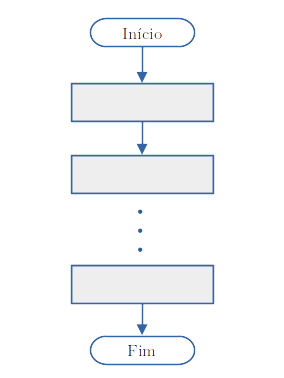
\includegraphics[width=0.4\textwidth]{./cap_progest/dados/fig_fg_sequencia/fig}
  \caption{Estrutura de sequência de blocos.}
  \label{cap_progest:fig:fg_sequencia}
\end{figure}

\begin{ex}
  O seguinte código computada a área do triângulo de base e altura informadas pela(o) usuária(o).
\begin{lstlisting}
#início

# bloco: entrada de dados
base = float(input('Digite a base:\n'))
altura = float(input('Digite a altura\n'))

# bloco: computação da área
area = base*altura/2

# bloco: saída de dados
print(f'Área = {area}')

#fim
\end{lstlisting}

  O código acima está estruturado em três blocos. O primeiro bloco (linhas 3-5) processa a entrada de dados, seu término ocorre somente após a(o) usuária(o) digitar os valores da base e da altura. Na sequência, o bloco (linhas 7-8) faz a computação da área do triângulo e aloca o resultado na variável \lstinline+area+. No que este bloco termina seu processamento, é executado o último bloco (linhas 10-11), que imprime o resultado na tela.
\end{ex}

\subsection{Ramificação}

\hl{Estruturas de ramificação permitem a seleção de um mais blocos com base em condições lógicas}.

\begin{ex}\label{cap_progest_sec_est:ex:ramifica}
  O seguinte código lê um número inteiro digitado pela(o) usuária(o) e imprime uma mensagem no caso do número digitado ser par.
\begin{lstlisting}
#início

# entrada de dados
n = int(input('Digite um número inteiro:\n'))

# ramificação
if (n%2 == 0):
    print(f'{n} é par.')

#término
\end{lstlisting}
  Observamos que, no caso do número digitado não ser par, o programa termina sem nenhuma mensagem ser impressa. Esse é um exemplo de um bloco de ramificação, a instrução de ramificação (linha 7) testa a condição de \lstinline+n+ ser par. Somente no caso de ser verdadeiro, a instrução de impressão (linha 8) é executada. Após e impressão o programa é encerrado. No caso de \lstinline+n+ não ser par, o programa é encerrado sem que a instrução da linha 8 seja executada, i.e. a mensagem não é impressa.

\begin{figure}[H]
  \centering
  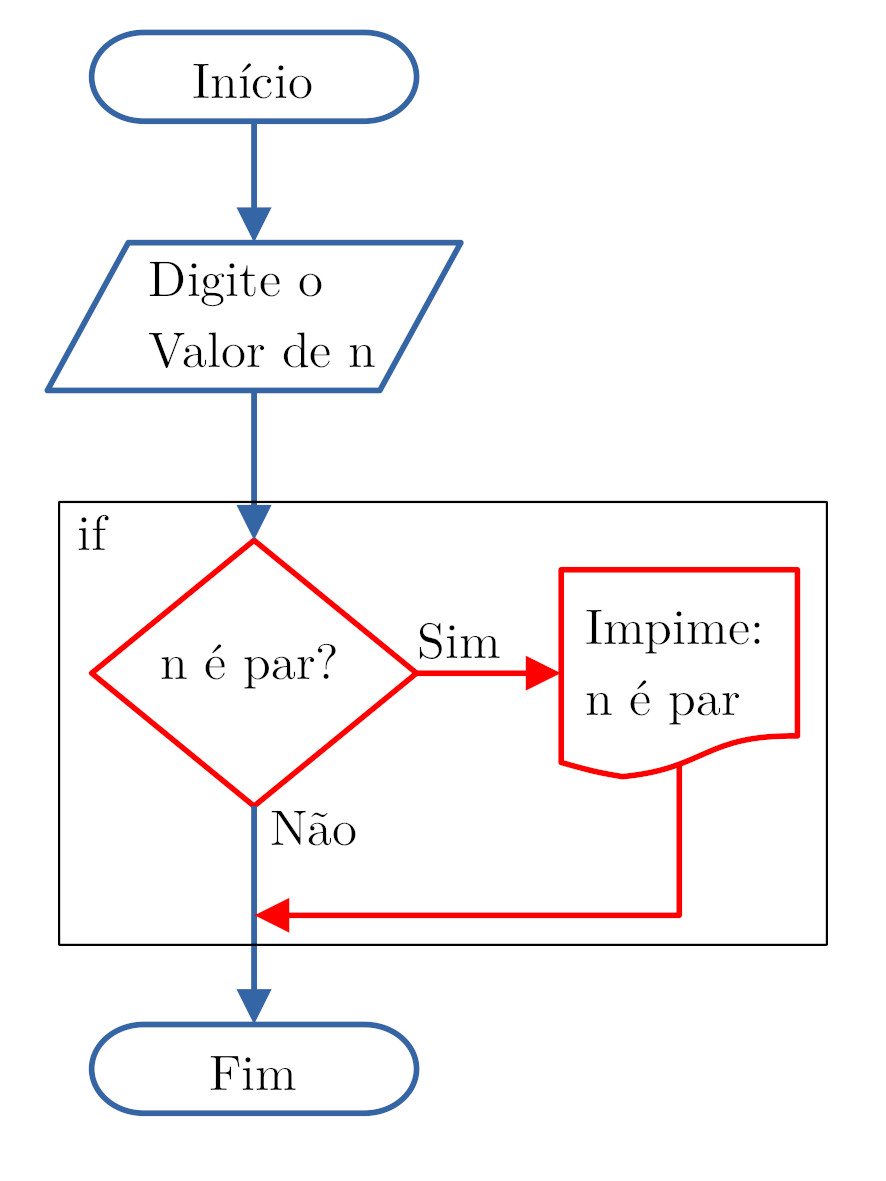
\includegraphics[width=0.5\textwidth]{./cap_progest/dados/fig_fg_ramifica/fig}
  \caption{Fluxograma de uma estrutura de ramificação.}
  \label{cap_progest:fig:fg_ramifica}
\end{figure}
  
\end{ex}

\begin{obs}\normalfont{\hl{(Escopo e indentação.)}}
  Na linguagem {\python}, a \href{https://pt.wikipedia.org/wiki/Indenta\%C3\%A7\%C3\%A3o}{indentação} indica o \emph{escopo}, i.e. o início e fim do bloco de instruções que pertencem a ramificação. No Exemplo \ref{cap_progest_sec_est:ex:ramifica}, o escopo da instrução \lstinline+if+ é apenas a linha 8.
\end{obs}

\subsection{Repetição}

\hl{Instruções de repetição permitem que um mesmo bloco seja processado várias vezes em sequência}. Em {\python}, há duas instruções de repetição disponíveis: \lstinline+for+ e \lstinline+while+. 

\subsubsection{\lstinline+for+}

A instrução \hl{{\lstinline+for+} permite que um bloco seja iterado para cada elemento de uma dada coleção de dados}.

\begin{ex}\label{cap_progest_sec_est:ex:for}
  O seguinte código testa a paridade de cada um dos elementos do conjunto $\{-3, -2, -1, 0, 1, 2, 3\}$.
\begin{lstlisting}
#início

# repetição for
for n in {-3, -2, -1, 0, 1, 2, 3}:
    res = (n%2 == 0)
    print(f'{n} é par? ', res)
    
#término
\end{lstlisting}
  A instrução de repetição \lstinline+for+ (linha 4), aloca em \lstinline+n+ um dos elementos do conjunto. Então, executa em sequência o bloco de comandos das linhas 5 e 6. De forma iterada, \lstinline+n+ recebe um novo elemento do conjunto e o bloco das linhas 5 e 6 é novamente executado. A repetição termina quando todos os elementos do conjunto já tiverem sido iterados. O código segue, então, para a linha 7. Não havendo mais instruções, o programa é encerrado.

\begin{figure}[H]
  \centering
  \includegraphics[width=0.6\textwidth]{./cap_progest/dados/fig_fg_for/fig}
  \caption{Fluxograma de uma estrutura de repetição do tipo \lstinline+for+.}
  \label{cap_progest_sec_est:fig:fg_for}
\end{figure}

Assim como no caso de uma instrução de ramificação, o escopo do \lstinline+for+ é definido pela indentação do código. Neste exemplo, o escopo são as linhas 5 e 6.
\end{ex}

[[tag:construcao]]

\subsubsection{\lstinline+while+}

A instrução \hl{{\lstinline+while+}, permite a repetição de um bloco enquanto uma dada condição lógica é satisfeita}.

\begin{ex}\label{cap_progest_sec_est:ex:while}
  O seguinte código testa a paridade dos números inteiros compreendidos de $-3$ a $3$.
\begin{lstlisting}
#início

n = -3

# repetição: while
while (n <= 3):
    res = (n%2 == 0)
    print(f'{n} é par?', res)
    n += 1
    
#término
\end{lstlisting}
  A instrução de repetição \lstinline+while+ faz com que o bloco de processamento definido pelas linhas 7-9 seja executado de forma sequencial enquanto o valor de \lstinline+n+ for menor ou igual a 3. No caso dessa condição ser verdadeira, o bloco (linhas 7-9) é executado e, então a condição é novamente verificada. No caso da condição ser falsa, esse bloco não é executado e o código segue para a linha 10. Não havendo mais nenhuma instrução, o programa é encerrado.

  \begin{figure}[H]
    \centering
    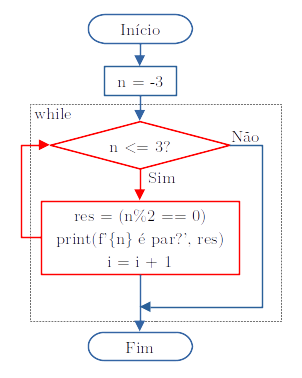
\includegraphics[width=0.6\textwidth]{./cap_progest/dados/fig_fg_while/fig}
    \caption{Fluxograma de uma estrutura de repetição do tipo \lstinline+while+.}
    \label{cap_progest_sec_est:fig:fg_while}
  \end{figure}

  Observamos que, neste exemplo, o escopo da instrução \lstinline+while+ são as linhas 7-9, determinado indentação do código.
\end{ex}

\subsection{Exercícios}

\begin{exer}
  Seja a reta de equação
  \begin{equation}
    y = ax + b.
  \end{equation}
  Assumindo $a=2$ e $b=-3$, o seguinte código foi desenvolvido para computar o ponto $x$ de interseção da desta reta com o eixo das abscissas.
\begin{lstlisting}
x = -b/(2*a)
a = 2
b = -3
print(x)
\end{lstlisting}
  Identifique e explique os erros desse código. Então, apresente uma versão corrigida.
\end{exer}
\begin{resp}
\begin{lstlisting}
a = 2
b = -3
x = -b/(2*a)
print(x)
\end{lstlisting}
\end{resp}

\begin{exer}\label{cap_progest_sec_est:exer:ramifica_reta}
  Seja a reta de equação
  \begin{equation}
    y = ax + b.
  \end{equation}
  Faça um fluxograma de um programa em que a(o) usuária(o) entra com os valores de $a$ e $b$. No caso de $a\neq 0$, o programa computa e imprime o ponto $x$ da interseção dessa reta com o eixo das abscissas.
\end{exer}
\begin{resp}
  Dica: consulte o Exemplo \ref{cap_progest_sec_est:ex:ramifica}.
\end{resp}

\begin{exer}
  Implemente o código referente ao fluxograma criado no Exercício \ref{cap_progest_sec_est:exer:ramifica_reta}.
\end{exer}
\begin{resp}
\begin{lstlisting}
a = float(input('Digite o valor de a:\n'))
b = float(input('Digite o valor de b:\n'))
if (a != 0):
    x = -b/(2*a)
    print(f'Ponto de interseção com o eixo x = {x}')
\end{lstlisting}
\end{resp}

\begin{exer}\label{cap_progest_sec_est:exer:for}
  Faça o fluxograma de um programa que usa de um bloco de repetição \lstinline+for+ para percorrer o conjunto
  \begin{equation}
    A = \{-4, -3, -2, -1, 0, 1, 2, 3, 4\}.
  \end{equation}
  A cada iteração, o programa imprime \lstinline+True+ ou \lstinline+False+ conforme o elemento seja ímpar ou não.
\end{exer}
\begin{resp}
  Dica: consulte o Exemplo \ref{cap_progest_sec_est:ex:for}.
\end{resp}

\begin{exer}
  Implemente o código referente ao fluxograma criado no Exercício \ref{cap_progest_sec_est:exer:for}.
\end{exer}
\begin{resp}
\begin{lstlisting}
A = {-4, -3, -2, -1, \
     0, 1, 2, 3, 4}
for x in A:
    res = (x % 2 != 0)
    print(f'{x} é ímpar? {res}')
\end{lstlisting}
\end{resp}

\begin{exer}\label{cap_progest_sec_est:exer:while}
  Faça um fluxograma análogo ao do Exercício \ref{cap_progest_sec_est:exer:for} que use a instrução de repetição \lstinline+while+ no lugar de \lstinline+for+.
\end{exer}
\begin{resp}
  Dica: consulte o Exemplo \ref{cap_progest_sec_est:ex:while}.
\end{resp}

\begin{exer}
  Implemente um código referente ao fluxograma criado no Exercício \ref{cap_progest_sec_est:exer:while}.
\end{exer}
\begin{resp}
\begin{lstlisting}
A = {-4, -3, -2, -1, \
     0, 1, 2, 3, 4}
n = -4
while (n <= 4):
    res = (n % 2 != 0)
    print(f'{n} é ímpar? {res}')
    n += 1
\end{lstlisting}
\end{resp}

\section{Instruções de Ramificação}\label{cap_progest_sec_ramifica}

[[tag:construcao]]

\subsection{Exercícios}

[[tag:construcao]]
% Este trabalho está licenciado sob a Licença Atribuição-CompartilhaIgual 4.0 Internacional Creative Commons. Para visualizar uma cópia desta licença, visite http://creativecommons.org/licenses/by-sa/4.0/deed.pt_BR ou mande uma carta para Creative Commons, PO Box 1866, Mountain View, CA 94042, USA.

\chapter{Funções}\label{cap_fun}
\thispagestyle{fancy}

Uma \hl{\emph{função} (ou método) é um \emph{subprograma} (ou subalgoritmo)}, um bloco de programação para o processamento de uma tarefa e que pode ser chamado à execução, sempre que necessário, pelo programa a que pertence.

\section{Funções Predefinidas e Módulos}\label{cap_fun_sec_buildin}

\subsection{Funções Predefinidas}

Como o nome indica, \hl{\emph{funções predefinidas} são aquelas disponíveis por padrão na linguagem de programação}, i.e. sem a necessidade de serem explicitamente definidas no código. As \hl{funções predefinidas do {\python}} podem ser consultadas em
\begin{center}
  \url{https://docs.python.org/3/library/functions.html}
\end{center}

Nós já vinhamos utilizando várias dessas funções.

\subsubsection{Entrada e Saída de Dados}

Na entrada e saída de dados, utilizamos
\begin{itemize}
\item \hl{{\lstinline+input()+}}

  Essa função lê uma linha digitada no \textit{prompt}, converte-a em uma \textit{string} e a retorna. Admite como entrada uma \textit{string} que é impressa no \textit{prompt} antes da leitura.

\item \hl{{\lstinline+print()+}}

  Essa função recebe um objeto e o imprime em formato texto, por padrão, no \textit{prompt} de saída.

\begin{lstlisting}
>>> s = input('Olá, qual o seu nome? ')
Olá, qual o seu nome? Fulane
>>> print(f'Bem vinde, {s}!')
Bem vinde, Fulane!
\end{lstlisting}
\end{itemize}

\subsubsection{Construtores de Dados}

Temos as funções que constroem objetos de classes de números:
\begin{itemize}

\item \hl{{\lstinline+bool()+}}

  Recebe um objeto e retorna outro da classe \lstinline+bool+.

\begin{lstlisting}
>>> bool(0)
False
>>> bool(1)
True
>>> bool('')
False
>>> bool('0')
True
\end{lstlisting}
  
\item \hl{{\lstinline+int()+}}

  Recebe um número ou \textit{string} \lstinline+x+ e retorna um objeto da classe \lstinline+int+.

\begin{lstlisting}
>>> int(-2.1)
-2
>>> int(3.9)
3
>>> int(5.5)
5
>>> int('51')
51
\end{lstlisting}

\item \hl{{\lstinline+float()+}}

  Recebe um número ou \textit{string} \lstinline+x+ e retorna um objeto da classe \lstinline+float+.

\begin{lstlisting}
>>> float(1)
1.0
>>> float('-2.7')
-2.7
\end{lstlisting}

\item \hl{{\lstinline+complex()+}}

  Recebe as partes real e imaginária de um número complexo ou uma \textit{string} e retorna um objeto da classe \lstinline+complex+.

\begin{lstlisting}
>>> complex(2,-3)
(2-3j)
>>> complex('-7+5j')
(-7+5j)
\end{lstlisting}
\end{itemize}

Para a construção de objetos de classes de coleção de dados, temos:
\begin{itemize}
\item \hl{{\lstinline+dict()+}}

  Recebe um mapeamento ou um iterável e retorna um objeto da classe \lstinline+dict+.

\item \hl{{\lstinline+list()+}}

  Recebe um iterável e retorna um objeto da classe \lstinline+list+.

\item \hl{{\lstinline+set()+}}

  Recebe um iterável e retorna um objeto da classe \lstinline+set+.

\item \hl{{\lstinline+str()+}}

  Recebe um objeto e retorna um outro da classe \lstinline+str+

\item \hl{{\lstinline+tuple+}}

  Recebe um iterável e retorna um objeto da classe \lstinline+tuple+.
\end{itemize}

Alguns construtores de iteráveis especiais são:
\begin{itemize}
\item \hl{{\lstinline+range()+}}

  Recebe até três inteiros \lstinline+start+, \lstinline+stop+, \lstinline+step+ e retorna um objeto iterável com início em \lstinline+start+ (incluído) e término em \lstinline+stop+ (excluído).

\begin{lstlisting}
>>> list(range(5))
[0, 1, 2, 3, 4]
>>> tuple(range(-10,1,2))
(-10, -8, -6, -4, -2, 0)
\end{lstlisting}

\item \hl{{\lstinline+enumerator()+}}

  Recebe um iterável e retorna um objeto \lstinline+enumerate+, um iterável de tuples que enumera os objetos do iterável de entrada.

\begin{lstlisting}
>>> cores = ['amarelo', 'azul', 'vermelho', ]
>>> list(enumerate(cores))
[(0, 'amarelo'), (1, 'azul'), (2, 'vermelho')]
\end{lstlisting}
\end{itemize}

\subsection{Módulos}

\hl{Módulos são bibliotecas computacionais}, i.e. um arquivo contendo funções (e/ou constantes) que podem ser incorporadas e usadas em outros programas. Existem vários módulos disponíveis na linguagem {\python}, para citar alguns:
\begin{itemize}
\item \hl{{\lstinline+math+}} : módulo de matemática elementar.
\item \hl{{\lstinline+random+}} : módulo de números randômicos.
\item \hl{{\lstinline+numpy+}} : módulo de computação matricial.
\item \hl{{\lstinline+matplotlib+}} : módulo de vizualização gráfica.
\item \hl{{\lstinline+sympy+}} : módulo de matemática simbólica.
\item \hl{{\lstinline+torch+}} : módulo de aprendizagem de máquina.
\end{itemize}

Nesta seção vamos apenas introduzir o módulo \lstinline+math+. Mais a frente, também fazemos uma introdução aos módulos \lstinline+numpy+ e \lstinline+matplotlib+.

\subsubsection{Módulo \lstinline+math+}

\hl{O módulo {\lstinline+math+} fornece acesso a constantes e funções matemáticas elementares para números reais}. Para \hl{\emph{importar o módulo}} em nosso código, podemos usar a instrução \hl{{\lstinline+import+}}. Por exemplo,
\begin{lstlisting}
>>> import math
>>> help(math)
\end{lstlisting}
Então, para usar algum recurso do módulo usamos \hl{{\lstinline+math.+}} seguido do nome do recurso que queremos. Por exemplo,
\begin{lstlisting}
>>> math.e
2.718281828459045
\end{lstlisting}
retorna o número de Euler{\euler} em ponto flutuante.

Alternativamente, podemos importar o módulo com o nome que quisermos. Por padrão, usa-se
\begin{lstlisting}
>>> import math as m
>>> m.pi
3.141592653589793
\end{lstlisting}
Ainda, pode-se importar apenas um ou mais recursos específicos, por exemplo\footnote{\faIcon[regular]{grin-wink}}
\begin{lstlisting}
>>> from math import pi, sin, cos
>>> sin(pi)**2 + cos(pi) == 1
False
\end{lstlisting}

\begin{ex}
  Considere um polinômio de segundo grau da forma
  \begin{equation}
    p(x) = ax^2 + bx + c.
  \end{equation}
  O seguinte código, computa as raízes de $p$ para valores dos coeficientes fornecidos por usuária(o).

\begin{lstlisting}
import math as m

# entrada de dados
a = float(input('Digite o valor de a:\n'))
b = float(input('Digite o valor de b:\n'))
c = float(input('Digite o valor de c:\n'))

# discriminante
delta = b**2 - 4*a*c

# raízes
# raízes distintas
if (delta > 0):
    x1 = (-b + m.sqrt(delta))/(2*a)
    x2 = (-b - m.sqrt(delta))/(2*a)
# raiz dupla
elif (delta == 0):
    x1 = -b/(2*a)
    x2 = x1
# raízes complexas
else:
    real = -b/(2*a)
    img = m.sqrt(-delta)/(2*a)
    x1 = complex(real, img)
    x2 = x1.conjugate()

print(f'x1 = {x1}')
print(f'x2 = {x2}')
\end{lstlisting}
\end{ex}

\subsection{Exercícios}

\begin{exer}
  Desenvolva um código que computa e imprime a hipotenusa $h$ de um triângulo retângulo com catetos $a$ e $b$ fornecidos por usuária(o).
\end{exer}
\begin{resp}
  Dica: use \lstinline+h = math.sqrt(a**2 + b**2)+.
\end{resp}

\begin{exer}
  Um triângulo de lados $a$, $b$ e $c$, existe se
  \begin{equation}
    |b-c| < a < b + c.
  \end{equation}
  Desenvolva um código que verifica e informa a existência de um triângulo de lados fornecidos por usuária(o).
\end{exer}
\begin{resp}
  Dica: verifique a condição \lstinline+(m.fabs(b-c) < a) and (a < b+c)+
\end{resp}

\begin{exer}
  Considere um triangulo com as seguintes medidas
  \begin{figure}[H]
    \centering
    \includegraphics[width=0.4\textwidth]{./cap_fun/dados/fig_leiDosCossenos/fig}
  \end{figure}
  Desenvolva um código que computa e imprime o valor da área de um triangulo de lados $a$, $b$ e $c$ fornecidos por usuária(o).
\end{exer}
\begin{resp}
  Dica: use a \href{https://pt.wikipedia.org/wiki/Lei_dos_cossenos}{lei dos cossenos} e relações fundamentais de triangulo retângulo para obter o valor da altura $h$. 
\end{resp}

\begin{exer}
  Desenvolva um código em que a(o) usuária forneça um ângulo $\theta$ em graus e seja computado e impresso os $\sen(\theta)$ e $\cos(\theta)$.
\end{exer}
\begin{resp}
  Dica: consulte as funções \lstinline+math.sin+, \lstinline+math.cos+.
\end{resp}

\begin{exer}
  Desenvolva um jogo em que a(o) usuária(o) tenha três tentativas para adivinhar um número inteiro entre $0$ a $51$ (incluídos). 
\end{exer}
\begin{resp}
  Dica: O módulo \lstinline+random+ fornece a função \href{https://docs.python.org/3/library/random.html?highlight=random#random.randint}{\lstinline+random.randint(a, b)+} que retorna um inteiro $a \leq x \leq b$.
\end{resp}

\section{Definindo Funções}\label{cap_fun_sec_def}

Em {\python}, criamos ou \hl{definimos uma função com a instrução {\lstinline+def+}}, com a seguinte sintaxe
\begin{lstlisting}
def foo(x):
   bloco
\end{lstlisting}
Aqui, \lstinline+foo+ é o nome da função, \lstinline+x+ é o parâmetro (variável) de entrada e \lstinline+bloco+ é o bloco de programação que a função executa ao ser chamada. Uma função pode ter mais parâmetros ou não ter parâmetro de entrada.

\begin{ex}\label{cap_fun_sec_def:ex:areaCirc}
  O seguinte código, define a função \lstinline+areaCirc+ que computa e imprime a área de uma circunferência de raio $r$.
\begin{lstlisting}
import math as m

def areaCirc(r):
    area = m.pi * r**2
    print(f'área = {area}')
\end{lstlisting}
  Uma vez definida, a função pode ser chamada em qualquer parte do código. Por exemplo, vamos continuar o código de forma que a(o) usuária(o) informe os raios de duas circunferências e o código compute e imprima o valor das áreas de cada circunferência.
\begin{lstlisting}
import math as m

# def fun
def areaCirc(r):
    area = m.pi * r**2
    print(f'área = {area}')
    
# entrada de dados
raio1 = float(input('Digite o raio da 1. circ.:\n'))
raio2 = float(input('Digite o raio da 2. circ.:\n'))

print(f'Circunferência de raio = {raio1}')
areaCirc(raio1)

print(f'Circunferência de raio = {raio2}')
areaCirc(raio2)
\end{lstlisting}
\end{ex}

\begin{obs}\normalfont{(\hl{{\lstinline+docstring+}}.)}
  {\python} recomenda a utilização do sistema de documentação \lstinline+docstring+. Na definição de funções, um pequeno comentário sobre sua funcionalidade, seguido da descrição sobre seus parâmetros podem ser feito usando \lstinline+'''+, logo abaixo da instrução \lstinline+def+. Por exemplo,
\begin{lstlisting}
import math as m

# def fun
def areaCirc(r):
    '''
    Computa e imprime a área de uma
    circunferência.

    Entrada
    -------
    r : float
    Raio da circunferência.
    '''
    area = m.pi * r**2
    print(f'área = {area}')
\end{lstlisting}
  Com isso, podemos usar a função \lstinline+help+ para obter a documentação da função \lstinline+areaCirc+.
\begin{lstlisting}
>>> help(areaCirc)
\end{lstlisting}
  Verifique!
\end{obs}

Uma função pode ser definida sem parâmetro de entrada.

\begin{ex}
  O seguinte código, implementa uma função que imprime um número randômico par entre $0$ e $100$ (incluídos).
\begin{lstlisting}
import random

def randPar100():
    '''
    Imprime um número randômico
    par entre 0 e 100 (incluídos).
    '''
    n = random.randint(0, 99)
    if (n % 2 == 0):
        print(n)
    else:
        print(n+1)
\end{lstlisting}
  Para chamá-la, usamos
\begin{lstlisting}
>>> randPar100()
\end{lstlisting}
  Verifique!
\end{ex}

\subsection{Funções com Saída de Dados}

Além de parâmetros de entrada, \hl{uma função pode ter saída de dados}, i.e. pode retornar dados para o programa. Para isso, usamos a instrução \lstinline+return+ que interrompe a execução da função e retorna ao programa principal. Quando o \lstinline+return+ é seguido de um objeto, a função tem como saída o valor desse objeto.

\begin{ex}
  Vamos atualizar a versão de nosso código do Exemplo \ref{cap_fun_sec_def:ex:areaCirc}. Aqui, em vez de imprimir, a função \lstinline+areaCirc(r)+ tem como saída o valor computado da área da circunferência de raio \lstinline+r+
\begin{lstlisting}
import math as m

# def fun
def areaCirc(r):
    area = m.pi * r**2
    return area
    
# entrada de dados
raio1 = float(input('Digite o raio da 1. circ.:\n'))
raio2 = float(input('Digite o raio da 2. circ.:\n'))

print(f'Circunferência de raio = {raio1}')
area1 = areaCirc(raio1)
print(f'\tárea = {area1}')

print(f'Circunferência de raio = {raio2}')
area2 = areaCirc(raio2)
print(f'\tárea = {area2}')
\end{lstlisting}
\end{ex}

Funções podem retornar objetos de qualquer classe de dados. Quando queremos retornar mais de um objeto por vez, usualmente usamos um \lstinline+tuple+ como variável de saída.

\begin{ex}
  O seguinte código, cria uma função para a computação das raízes de um polinômio de grau 2
  \begin{equation}
    p(x) = ax^2 + bx + c.
  \end{equation}
\begin{lstlisting}
import math as m

def raizes(a, b, c):
    '''
    Computa as raízes de
    p(x) = ax^2 + bx + c

    Entrada
    -------
    a : float
    Coeficiente do termo quadrático.
    Atenção! Deve ser diferente de zero.

    b : float 
    Coeficiente do termo linear.

    c: float
    Coeficiente do termo constante.

    Saída
    -----
    x1 : float
    Uma raíz do polinômio.

    x2 : float
    Outra raíz do polinômio.
    Atenção! No caso de raiz dupla,
    x1 == x2.
    '''

    # auxiliares
    _2a = 2*a
    _b2a = -b/_2a

    # discriminante
    delta = b**2 - 4*a*c

    # raízes
    if (delta > 0):
        x1 = _b2a + m.sqrt(delta)/_2a
        x2 = _b2a - m.sqrt(delta)/_2a
        return x1, x2
    elif (delta < 0):
        img = m.sqrt(-delta)/_2a
        x1 = _b2a + img*1j
        return x1, x1.conjugate()
    else:
        return _b2a, _b2a
\end{lstlisting}
  Verifique!
\end{ex}

\subsection{Capturando Exceções}

[[tag:construcao]]

\subsection{Criando um Módulo}

[[tag:construcao]]

\subsection{Exercícios}

\begin{exer}
  Defina uma função que retorna um número randômico ímpar entre $1$ e $51$ (incluídos). Use-a para escrever um código em que:
  \begin{enumerate}[1.]
  \item A(o) usuária(o) informa um número inteiro $n\geq 1$.
  \item Cria-se uma lista de $n$ números randômicos ímpares entre $1$ e $51$ (incluídos).
  \item Computa-se e imprime-se a média dos $n$ números.
  \end{enumerate}
\end{exer}
\begin{resp}
\begin{lstlisting}
import random

def randImpar(m=51):
    '''
    Retorna um número randômico
    ímpar entre 1 e m (incluídos).

    Entrada
    -------
    m : int
    Maior inteiro ímpar que pode ser 
    gerado. Padrão: m = 51.

    Saída
    -----
    n : int
    Número randômico ímpar.
    '''
    n = random.randint(0, m-1)
    if (n % 2 != 0):
        return n
    else:
        return n+1

# entrada de dados
n = int(input('Digite o tamanho da lista:\n'))

# gera a lista
lista = [0]*n
for i in range(n):
    lista[i] = randImpar()

# calcula a média
soma = sum(lista)
media = soma/len(lista)

# imprime o resultados
print(f'média = {media}')
\end{lstlisting}
\end{resp}
% Este trabalho está licenciado sob a Licença Atribuição-CompartilhaIgual 4.0 Internacional Creative Commons. Para visualizar uma cópia desta licença, visite http://creativecommons.org/licenses/by-sa/4.0/deed.pt_BR ou mande uma carta para Creative Commons, PO Box 1866, Mountain View, CA 94042, USA.

\chapter{Arranjos e Matrizes}\label{cap_arr}

\hl{Um arranjo é uma coleção de objetos} (todos de um mesmo tipo) \hl{em que os elementos são organizados por eixos}. É a estrutura de dados mais utilizada para a alocação de vetores e matrizes, fundamentais na computação matricial.

\section{Arranjos}\label{cap_arr_sec_arr}

\hl{Um arranjo (em inglês, \textit{array}) é uma coleção de objetos (todos do mesmo tipo) em que os elementos são organizados por eixos}. Nesta seção, vamos nos restringir a \hl{\emph{arranjos unidimensionais}} (de apenas um eixo). Esta é a estrutura computacionais usualmente utilizada \hl{para a alocação de vetores}.

\hl{{\numpy} é uma biblioteca {\python} que fornece suporte para a alocação e manipulação de arranjos}. Usualmente, a biblioteca é importada como segue

\begin{lstlisting}
import numpy as np
\end{lstlisting}

Na sequência, vamos assumir que o {\numpy} já está importado como acima.

\subsection{Alocação de Arranjos}

O método {\PYTHONnumpyDOTarray} permite a \hl{alocação de um arranjo}. Como parâmetro de entrada, recebe uma {\PYTHONlist} contendo os elementos do arranjo. Por exemplo,

\begin{lstlisting}
>>> v = np.array([-2, 1, 3])
>>> v
array([-2,  1,  3])
>>> type(v)
<class 'numpy.ndarray'>
\end{lstlisting}

aloca o arranjo de números inteiros \lstinline+v+. Embora arranjos não sejam vetores, \hl{a modelagem computacional de vetores usualmente é feita utilizando-se} \texttt{arrays}. Por exemplo, em um código {\python}, o vetor
\begin{equation}
  \pmb{v} = (-2, 1, 3)
\end{equation}
pode ser alocado usando-se o \texttt{array} \lstinline+v+ acima.

O \hl{tipo dos dados} de um \lstinline+array+ é definido na sua criação. Pode ser feita de forma automática ou explícita pela propriedade {\PYTHONnumpyDOTdtype}. Por exemplo,

\begin{lstlisting}
>>> v = np.array([-2, 1, 3])
>>> v.dtype
dtype('int64')
>>> v = np.array([-2., 1, 3])
>>> v.dtype
dtype('float64')
>>> v = np.array([-2, 1, 3], dtype='float')
>>> v.dtype
dtype('float64')
\end{lstlisting}

\begin{ex}
  Aloque o vetor
  \begin{equation}
    \pmb{v} = (\pi, 1, e)
  \end{equation}
  como um \lstinline+array+ do {\numpy}.

\begin{lstlisting}
>>> import numpy as np
>>> v = np.array([np.pi, 1, np.e])
>>> v
array([3.14159265, 1.        , 2.71828183])
\end{lstlisting}

\end{ex}

O {\numpy} conta com \hl{métodos úteis para a \emph{inicialização}} de \texttt{arrays}:
\begin{itemize}
\item {\PYTHONnumpyDOTzeros} \hlemph{arranjo de elementos nulos}

\begin{lstlisting}[xrightmargin=2.5em]
>>> np.zeros(3)
array([0., 0., 0.])
\end{lstlisting}

\item {\PYTHONnumpyDOTones} \hlemph{arranjo de elementos iguais a um}

\begin{lstlisting}[xrightmargin=2.5em]
>>> np.ones(2, dtype='int')
array([1, 1])
\end{lstlisting}

\item {\PYTHONnumpyDOTempty} \hlemph{arranjo de elementos não predefinidos}

\begin{lstlisting}[xrightmargin=2.5em]
>>> np.empty(3)
array([4.64404327e-310, 0.00000000e+000, 6.93315702e-310])
\end{lstlisting}

\item {\PYTHONnumpyDOTlinspace}\texttt{(start, stop, num=50)} \emph{\hl{arranjo de elementos uniformemente espaçados}}

\begin{lstlisting}[xrightmargin=2.5em]
>>> np.linspace(0, 1, 5)
array([0.  , 0.25, 0.5 , 0.75, 1.  ])
\end{lstlisting}
\end{itemize}

\subsection{Indexação e Fatiamento}\label{cap_arr_sec_arr:ssec:islice}

Um {\PYTHONnumpyDOTarray} é uma \hl{coleção de objetos mutável, ordenada e indexada}. Indexação e fatiamento podem ser feitos da mesma forma que para um {\PYTHONtuple} ou uma {\PYTHONlist}. Por exemplo,

\begin{lstlisting}
>>> v = np.array([-1, 1, 2, 0, 3])
>>> v[0]
-1
>>> v[-1]
3
>>> v[1:4]
array([1, 2, 0])
>>> v[::-1]
array([ 3,  0,  2,  1, -1])
>>> v[3] = 4
>>> v
array([-1,  1,  2,  4,  3])
\end{lstlisting}

\subsection{Reordenamento dos Elementos}

Em programação, o reordenamento (em inglês, \textit{sorting}) de elementos de uma sequência ordenada de números (\texttt{array}, \texttt{tuple}, \texttt{tuple}, etc.) consiste em alterar a sequência de forma que os elementos sejam organizados do menor para o mair valor. Na sequência, vamos estudar alguns métodos para isso.

\subsubsection{Método Bolha}

Dado um {\PYTHONnumpyDOTarray}\endnote{Ou, um {\PYTHONtuple}, {\PYTHONlist}, etc..}, o método bolha consiste em percorrer o arranjo e permutar dois elementos consecutivos de forma que o segundo seja sempre maior que o primeiro. Uma vez que percorrermos o arranjo, teremos garantido que o maior valor estará na última posição do arranjo e os demais elementos ainda poderão estar desordenados. Então, percorremos o arranjo novamente, permutando elementos dois-a-dois conforme a ordem desejada, o que trará o segundo maior elemento para a penúltima posição. Ou seja, para um arranjo com $n$ elementos, temos garantido o reordenamento de todos os elementos após $n-1$ repetições desse algoritmo.

\begin{ex}
  Na sequência, implementamos o Método Bolha para o reordenamento de arranjos e aplicamos para
  \begin{equation}
    \pmb{v} = (-1, 1, 0, 4, 3).
  \end{equation}
  
\begin{lstlisting}[caption=bubbleSort\_v1.py]
import numpy as np

def bubbleSort(arr):
    arr = arr.copy()
    n = len(arr)
    for k in range(n-1):
        for i in range(n-k-1):
            if (arr[i] > arr[i+1]):
                arr[i], arr[i+1] = arr[i+1], arr[i]
    return arr

v = np.array([-1,1,0,4,3])
w = bubbleSort(v)
print(w)
\end{lstlisting}

\end{ex}

\begin{obs}
  Em geral, para um arranjo de $n$ elementos, o Método Bolha requer $n-1$ repetições para completar o ordenamento. Entretanto, dependendo do caso, o ordenamento dos elementos pode terminar em menos passos.
\end{obs}

\begin{ex}
  Na sequência, implementamos uma nova versão do Método Bolha para o reordenamento de arranjos. Esta versão verifica se há elementos fora de ordem e, caso não haja, interrompe o algoritmo. Como exemplo, aplicamos para
  \begin{equation}
    \pmb{v} = (-1, 1, 0, 4, 3).
  \end{equation}
  
\begin{lstlisting}[caption=bubbleSort\_v2.py]
import numpy as np

def bubbleSort(arr):
    arr = arr.copy()
    n = len(arr)
    for k in range(n-1):
        noUpdated = True
        for i in range(n-k-1):
            if (arr[i] > arr[i+1]):
                arr[i], arr[i+1] = arr[i+1], arr[i]
                noUpdated = False
        if (noUpdated):
            break
    return arr

v = np.array([-1,1,0,4,3])
w = bubbleSort(v)
\end{lstlisting}

\end{ex}

\begin{obs}\normalfont{(\hl{Métodos de Ordenamento}.)}
  Existem vários métodos para o ordenamento de uma sequência. O Método Bolha é um dos mais simples, mas também, em geral, menos eficiente. O {\numpy} tem disponível a função {\PYTHONnumpyDOTsort} para o reordenamento de elementos. Também bastante útil, é a função {\PYTHONnumpyDOTargsort}, que retorna os índices que reordenam os elementos.
\end{obs}

\subsection{Operações Elemento-a-Elemento}

No {\numpy}, temos os \hlemph{operadores aritméticos elemento-a-elemento} (em ordem de precedência)
\begin{itemize}
\item \lstinline!**!

\begin{lstlisting}[xrightmargin=2.5em]
>>> v = np.array([-2., 1, 3])
>>> w = np.array([1., -1, 2])
>>> v ** w
array([-2.,  1.,  9.])
\end{lstlisting}

\item \lstinline!*!, \lstinline!/!, \lstinline!//!, \lstinline!%!

\begin{lstlisting}[xrightmargin=2.5em]
>>> v * w
array([-2., -1.,  6.])
>>> v / w
array([-2. , -1. ,  1.5])
>>> v // w
array([-2., -1.,  1.])
>>> v % w
array([ 0., -0.,  1.])
\end{lstlisting}

\item \lstinline!+!, \lstinline!-!

\begin{lstlisting}[xrightmargin=2.5em]
>>> v + w
array([-1.,  0.,  5.])
>>> v - w
array([-3.,  2.,  1.])
\end{lstlisting}

\end{itemize}

\begin{ex}
  Vamos usar \texttt{arrays} para alocar os vetores
  \begin{align}
    \pmb{v} = (1., 0, -2),\\
    \pmb{w} = (2., -1, 3).
  \end{align}
  Então, computamos o produto interno
  \begin{subequations}
    \begin{align}
      \pmb{v}\cdot\pmb{w} &:= v_1w_1 + v_2w_2 + v_3w_3\\
                          &= 1\cdot 2 + 0\cdot(-1) + (-2)\cdot 3\\
                          &= -4.
    \end{align}
  \end{subequations}

\begin{lstlisting}
import numpy as np
# vetores
v = np.array([1., 0, -2])
w = np.array([2., -1, 3])
# produto interno
vdw = np.sum(v*w)
\end{lstlisting}

\end{ex}

\begin{obs}\normalfont{(\hl{Concatenação de Arranjos}.)}
  No {\numpy}, a concatenação de arranjos pode ser feita com a função {\PYTHONnumpyDOTconcatenate}. Por exemplo,

\begin{lstlisting}
>>> v = np.array([1,2])
>>> w = np.array([3,4])
>>> np.concatenate((v,w))
array([1, 2, 3, 4])
\end{lstlisting}

\end{obs}

\subsection{Exercícios}

\begin{exer}
  Aloque cada um dos seguintes vetores como um {\PYTHONnumpyDOTarray}:
  \begin{enumerate}[a)]
  \item $\displaystyle\pmb{a} = (0, -2, 4)$
  \item $\displaystyle\pmb{b} = (0.1, -2.7, 4.5)$
  \item $\displaystyle\pmb{c} = (e, \ln(2), \pi)$
  \end{enumerate}
\end{exer}
\begin{resp}

\begin{lstlisting}
>>> import numpy as np
>>> a = np.array([0, -2, 4])
>>> b = np.array([0.1, -2.7, 4.5])
>>> c = np.array([np.e, np.log(2), np.pi])
\end{lstlisting}

\end{resp}

\begin{exer}
  Considere o seguinte {\PYTHONnumpyDOTarray}

\begin{lstlisting}
>>> v = np.array([4, -1, 1, -2, 3]).
\end{lstlisting}

Sem implementar, escreva os arranjos derivados:
  \begin{enumerate}[a)]
  \item \lstinline+v[1]+
  \item \lstinline+v[1:4]+
  \item \lstinline+v[:3]+
  \item \lstinline+v[1:]+
  \item \lstinline+v[1:4:2]+
  \item \lstinline+v[-2:-5:-1]+
  \item \lstinline+v[::-2]+
  \end{enumerate}
  Então, verifique seus resultados implementando-os.
\end{exer}
\begin{resp}
  Dica: consulte a Subseção \ref{cap_arr_sec_arr:ssec:islice}. 
\end{resp}

\begin{exer}
  Desenvolva uma função \lstinline+argBubbleSort(arr)+, i.e. uma função que retorna os índices que reordenam os elementos do arranjo \lstinline+arr+ em ordem crescente. Teste seu código para o ordenamento de diversos arranjos e compare os resultados com a aplicação da função {\PYTHONnumpyDOTargsort}.
\end{exer}
\begin{resp}

\begin{lstlisting}
import numpy as np

def argBubbleSort(arr):
    n = len(arr)
    ind = np.arange(n)
    for k in range(n-1):
        noUpdated = True
        for i in range(n-k-1):
            if (arr[ind[i]] > arr[ind[i+1]]):
                ind[i], ind[i+1] = ind[i+1], ind[i]
                noUpdated = False
        if (noUpdated):
            break
    return ind
\end{lstlisting}

\end{resp}

\begin{exer}
  Desenvolva um Método Bolha para o reordenamento dos elementos de um dado arranjo em ordem decrescente. Teste seu código para o reordenamento de diversos arranjos. Como pode-se usar a função {\PYTHONnumpyDOTsort} para obter os mesmos resultados?
\end{exer}
\begin{resp}

\begin{lstlisting}
import numpy as np

def emOrdem(x, y):
    return x < y

def bubbleSort(arr, emOrdem=emOrdem):
    arr = arr.copy()
    n = len(arr)
    for k in range(n-1):
        noUpdated = True
        for i in range(n-k-1):
            if not(emOrdem(arr[i], arr[i+1])):
                arr[i], arr[i+1] = arr[i+1], arr[i]
                noUpdated = False
        if (noUpdated):
            break
    return arr
\end{lstlisting}

\end{resp}

\begin{exer}
  Desenvolva uma função \lstinline+argBubbleSort(arr, emOrdem)+, i.e. uma função que retorna os índices que reordenam os elementos do arranjo \lstinline+arr+ na ordem definida pela função \lstinline+emOrdem+. Teste seu código para o ordenamento de diversos arranjos, tanto em ordem crescente como em ordem decrescente. Como pode-se obter os mesmos resultados usando-se a função {\PYTHONnumpyDOTargsort}?
\end{exer}
\begin{resp}

\begin{lstlisting}
import numpy as np

def argBubbleSort(arr, emOrdem=emOrdem):
    n = len(arr)
    ind = np.arange(n)
    for k in range(n-1):
        noUpdated = True
        for i in range(n-k-1):
            if not(emOrdem(arr[ind[i]], arr[ind[i+1]])):
                ind[i], ind[i+1] = ind[i+1], ind[i]
                noUpdated = False
        if (noUpdated):
            break
    return ind
\end{lstlisting}

\end{resp}

\begin{exer}
  Crie uma função \lstinline+media(arr)+ que returna o valor médio do arranjo de números \lstinline+arr+. Teste seu código para diferentes arranjos e compare os resultados com o da função {\PYTHONnumpyDOTmean}.
\end{exer}
\begin{resp}

\begin{lstlisting}
import numpy as np

def media(arr):
    return np.sum(arr)/len(arr)
\end{lstlisting}

\end{resp}

\begin{exer}
  Desenvolva uma função que retorna o ângulo entre dois vetores $\pmb{v}$ e $\pmb{w}$ dados.
\end{exer}
\begin{resp}

\begin{lstlisting}
import numpy as np

def dot(v, w):
    return np.sum(v*w)

def angulo(v, w):
    # norma de v
    norm_v = np.sqrt(dot(v,v))
    # norma de w
    norm_w = np.sqrt(dot(w,w))
    # cos(theta)
    cosTheta = dot(v,w)/(norm_v*norm_w)
    # theta
    theta = np.acos(cosTheta)
    return theta
\end{lstlisting}

\end{resp}

\ifisbook
\subsubsection{Respostas}
\shipoutAnswer
\fi


\section{Vetores}\label{cap_arr_sec_vetor}

O uso de \texttt{arrays} é uma das formas mais adequadas para fazermos a \hl{modelagem computacional de \emph{vetores}}. Entretanto, devemos ficar atentos que \hl{vetores e arranjos não são equivalentes}. Embora, a soma/subtração e multiplicação por escalar são similares, a multiplicação e potenciação envolvendo vetores não estão definidas, mas para arranjos são operações elemento-a-elemento.

No que segue, vamos assumir que a biblioteca {\numpy} está importada, i.e.

\begin{lstlisting}
>>> import numpy as np
\end{lstlisting}

\begin{ex}
  Podemos alocar os vetores
  \begin{align}
    &\pmb{v} = (1, 0, -2),\\
    &\pmb{w} = (2, -1, 3),
  \end{align}
  como \texttt{arrays} do {\numpy}

\begin{lstlisting}
>>> v = np.array([1, 0, -2])
>>> w = np.array([2, -1, 3])
\end{lstlisting}

  A soma dos vetores é uma operação elemento-a-elemento
  \begin{subequations}
    \begin{align}
      \pmb{v}+\pmb{w} &= (1, 0, -2) + (2, -1, 3)\\
                      &= \left(1+2, 0+(-1), -2+3\right)\\
                      &= (3, -1, 1)
    \end{align}
  \end{subequations}
  e a dos \texttt{arrays} é equivalente

\begin{lstlisting}
>>> v+w
array([ 3, -1,  1])
\end{lstlisting}

  A subtração dos vetores também é uma operação elemento-a-elemento
  \begin{subequations}
    \begin{align}
      \pmb{v}-\pmb{w} &= (1, 0, -2) - (2, -1, 3)\\
                      &= \left(1-2, 0-(-1), -2-3\right)\\
                      &= (-1, 1, -5)
    \end{align}
  \end{subequations}
  e a dos \texttt{arrays} é equivalente

\begin{lstlisting}
>>> v-w
array([ -1, 1,  -5])
\end{lstlisting}

  Ainda, a multiplicação por escalar
  \begin{subequations}
    \begin{align}
      2\pmb{v} &= 2(1, 0, -2)\\
               &= \left(2\cdot 1, 2\cdot 0, 2\cdot(-2)\right)\\
               &= (2, 0, -4)
    \end{align}
  \end{subequations}
  também é feita elemento-a-elemento, assim como com \texttt{arrays}

\begin{lstlisting}
>>> 2*v
array([ 2,  0, -4])
\end{lstlisting}

  Agora, para vetores, a multiplicação $\pmb{v}\pmb{w}$, divisão $\pmb{v}/\pmb{w}$, potenciação $\pmb{v}^2$ não são operações definidas. Diferentemente, para arranjos são operações elemento-a-elemento

\begin{lstlisting}
>>> v*w
array([ 2,  0, -6])
>>> v/w
array([ 0.5, -0., -0.66666667])
>>> v**2
array([1, 0, 4])
\end{lstlisting}

\end{ex}

\subsection{Funções Vetoriais}

Funções vetoriais $f:\mathbb{R}^n\to\mathbb{R}^n$ e funcionais $f:\mathbb{R}^n\to\mathbb{R}$ também podem ser adequadamente modeladas com o emprego de \texttt{arrays} do \hl{{\numpy}}. A biblioteca também \hl{conta com várias funções matemáticas predefinidas}, consulte
\begin{center}
  \url{https://numpy.org/doc/stable/reference/routines.math.html}
\end{center}

\begin{ex}\normalfont{(\hl{Função Vetorial}.)}
  A implementação da função vetorial $\pmb{f}:\mathbb{R}^3\to\mathbb{R}^3$
  \begin{equation}
    \pmb{f}(\pmb{x}) = (x_1^2+\sin(x_1), x_2^2+\sin(x_2), x_3^2+\sin(x_3))
  \end{equation}
  para $\pmb{x} = (x_1, x_2, x_3)\in\mathbb{R}^3$, pode ser feita da seguinte forma

\begin{lstlisting}
import numpy as np

def f(x):
    return x**2 + np.sin(x)

# exemplo
x = np.array([0, np.pi, np.pi/2])
print(f'y = {f(x)}')
\end{lstlisting}

Verifique!
\end{ex}

\subsection{Produto Interno}

O \hlemph{produto interno} (ou, produto escalar) é a operação entre vetores $\pmb{v},\pmb{w}\in\mathbb{R}^n$ definida por
\begin{equation}
  \pmb{v}\cdot\pmb{v} := v_1w_1+v_2w_2+\cdots+v_nw_n.
\end{equation}
A função {\PYTHONnumpyDOTdot} computa o produto interno dos \texttt{arrays}.

\begin{ex}
  Consideramos os vetores
  \begin{align}
    &\pmb{v} = (1, 0, -2),\\
    &\pmb{w} = (2, -1, 3).
  \end{align}
  O produto interno desses vetores é
  \begin{subequations}
    \begin{align}
    \pmb{v}\cdot\pmb{w} &= v_1w_1 + v_2w_2 + v_3w_3\\
                        &= 1\cdot 2 + 0\cdot(-1) + (-2)\cdot 3\\
                        &= 2 + 0 -6 = -4
    \end{align}
  \end{subequations}
  Usando \texttt{arrays}, temos

\begin{lstlisting}
>>> v = np.array([1, 0, -2])
>>> w = np.array([2, -1, 3])
>>> np.sum(v*w)
-4
>>> np.dot(v,w)
-4
\end{lstlisting}

\end{ex}

\subsection{Norma de Vetores}

A \hl{\emph{norma} $L^2$ de um vetor} $\pmb{v}\in\mathbb{R}^n$ é definida por
\begin{equation}
  \|\pmb{v}\| := \sqrt{v_1^2+v_2^2+\cdots+v_n^2}
\end{equation}
O \hl{submódulo de álgebra linear} {\PYTHONnumpyDOTlinalg} contém a função {\PYTHONnumpyDOTlinalgDOTnorm} para a computação da norma de \texttt{arrays}.

\begin{ex}
  A norma do vetor $\pmb{v} = (3, 0, -4)$ é
  \begin{subequations}
    \begin{align}
      \|\pmb{v}\| &= \sqrt{v_1^2 + v_2^2 + v_3^2}\\
                  &= \sqrt{3^2 + 0^2 + (-4)^2}\\
                  &= \sqrt{9 + 0 + 16}\\
                  &= \sqrt{25} = 5.
    \end{align}
  \end{subequations}
  Usando o módulo {\PYTHONnumpyDOTlinalg}, obtemos

\begin{lstlisting}
>>> import numpy as np
>>> import numpy.linalg as npla
>>> v = np.array([3, 0, -4])
>>> np.sqrt(np.dot(v,v))
5.0
>>> npla.norm(v)
5.0
\end{lstlisting}

\end{ex}

\subsection{Produto Vetorial}

O \hl{\emph{produto vetorial}} entre dois vetores $\pmb{v}, \pmb{w}\in\mathbb{R}^3$ é definido por
\begin{subequations}
  \begin{align}
    \pmb{v}\times\pmb{w} &:=
                           \begin{vmatrix}
                             \pmb{i} & \pmb{j} & \pmb{k}\\
                             v_1 & v_2 & v_3\\
                             w_1 & w_2 & w_3
                           \end{vmatrix}\\
                         &=
                           \begin{vmatrix}
                             v_2 & v_3\\
                             w_2 & w_3
                           \end{vmatrix}\pmb{i}\\
                         &- \begin{vmatrix}
                             v_1 & v_3\\
                             w_1 & w_3
                           \end{vmatrix}\pmb{j}\\
                         &+ \begin{vmatrix}
                             v_1 & v_2\\
                             w_1 & w_2
                           \end{vmatrix}\pmb{k}\\
  \end{align}
\end{subequations}
A função {\PYTHONnumpyDOTcross} computa o \hl{produto vetorial} entre \texttt{arrays} (unidimensionais de 3 elementos).

\begin{ex}
  O produto vetorial entre os vetores $\pmb{v} = (1, -2, 1)$ e $\pmb{w} = (0, 2, -1)$ é
  \begin{subequations}
    \begin{align}
      \pmb{v}\times \pmb{w} &=
                              \begin{vmatrix}
                                \pmb{i} & \pmb{j} & \pmb{k}\\
                                1 & -2 & 1\\
                                0 & 2 & -1
                              \end{vmatrix}\\
                            &= 0\pmb{i} + \pmb{j} + 2\pmb{k}\\
                            &= (0, 1, 2).
    \end{align}
  \end{subequations}
    Com o {\numpy}, temos

\begin{lstlisting}
>>> v = np.array([1, -2, 1])
>>> w = np.array([0, 2, -1])
>>> np.cross(v,w)
array([0, 1, 2])
\end{lstlisting}

\end{ex}

\subsection{Exercícios}

\begin{exer}
  Considere os seguintes vetores
  \begin{align}
    &\pmb{u} = (2, -1, 1)\\
    &\pmb{v} = (1, -3, 2)\\
    &\pmb{w} = (-2, -1, -3)
  \end{align}
  Usando \texttt{arrays} do {\numpy}, compute:
  \begin{enumerate}[a)]
  \item $\pmb{u}\cdot\pmb{v}$
  \item $\pmb{u}\cdot (2\pmb{v})$
  \item $\pmb{u}\cdot (\pmb{w} + \pmb{v})$
  \item $\pmb{v}\cdot (\pmb{v} - 2\pmb{u})$
  \end{enumerate}
\end{exer}
\begin{resp}
  Dica: use a função $np.dot()$ e verifique as computações calculando os resultados esperados.
\end{resp}

\begin{exer}
  Considere os seguintes vetores
  \begin{align}
    &\pmb{u} = (2, -1, 1)\\
    &\pmb{v} = (1, -3, 2)\\
    &\pmb{w} = (-2, -1, -3)
  \end{align}
  Usando \texttt{arrays} do {\numpy}, compute:
  \begin{enumerate}[a)]
  \item $\|\pmb{u}\|$
  \item $\|\pmb{u} + \pmb{v}\|$
  \item $|\pmb{u}\cdot \pmb{w}|$
  \end{enumerate}
\end{exer}
\begin{resp}
  Dica: use a função {\PYTHONnumpyDOTlinalgDOTnorm} e verifique as computações calculando os resultados esperados.
\end{resp}

\begin{exer}
  Dados vetores $\pmb{u}$ e $\pmb{v}$, temos que
  \begin{equation}
    \pmb{u}\cdot\pmb{v} = \|\pmb{u}\|\|\pmb{v}\|\cos\theta,
  \end{equation}
  onde $\theta$ é o ângulo entre esses vetores. Implemente uma função que recebe dois vetores e retorna o ângulo entre eles. Teste seu código para diferentes vetores.
\end{exer}
\begin{resp}

\begin{lstlisting}
import numpy as np
import numpy.linalg as npla

def angulo(v, w):
    # \|v\|
    norm_v = npla.norm(v)
    # \|w\|
    norm_w = npla.norm(w)
    # u.v
    vdw = np.dot(v, w)
    # cos \theta
    ct = norm_v*norm_w/udw
    return np.acos(ct)
\end{lstlisting}

\end{resp}

\begin{exer}
  A projeção ortogonal do vetor $\pmb{u}$ na direção do vetor $\pmb{v}$ é definida por
  \begin{equation}
    \proj_{\pmb{v}} \pmb{u} := \frac{\pmb{u}\cdot\pmb{v}}{\|\pmb{v}\|^2}\pmb{v}.
  \end{equation}
  Implemente uma função que recebe dois vetores $\pmb{u}$, $\pmb{v}$ e retorne a projeção de $\pmb{u}$ na direção de $\pmb{v}$. Teste seu código para diferentes vetores.
\end{exer}
\begin{resp}

\begin{lstlisting}
import numpy as np
import numpy.linalg as npla

def proj(u, v):
    # \|v\|
    norm_v = npla.norm(v)
    # u.v
    udv = np.dot(u, v)
    # proj_v u
    proj_vu = udv/norm_v * v
    return proj_vu
\end{lstlisting}

\end{resp}

\begin{exer}
  Considere os vetores
  \begin{align}
    &\pmb{u} = (2, -3, 1),\\
    &\pmb{v} = (1, -2, -1).
  \end{align}
  Usando \texttt{arrays} do {\numpy}, compute os seguintes produtos vetoriais:
  \begin{enumerate}[a)]
  \item $\pmb{u}\times\pmb{v}$
  \item $\pmb{v}\times (2\pmb{v})$
  \end{enumerate}
\end{exer}
\begin{resp}
  Dica: use a função {\PYTHONnumpyDOTcross} e verifique as computações calculando os resultados esperados.
\end{resp}

\ifisbook
\subsubsection{Respostas}
\shipoutAnswer
\fi

\section{Arranjos Multidimensionais}\label{cap_arr_sec_multi}

\hl{Um arranjo {\PYTHONnumpyDOTarray} é um tabelamento de elementos de um mesmo tipo}. Os elementos são organizados por eixos indexados (em inglês, \textit{axes}). Enquanto que nas seções anteriores nos restringimos a \texttt{arrays} unidimensionais (de apenas um eixo), aqui, vamos estudar a alocação e manipulação de arranjos de vários eixos.

\subsection{Alocação, Indexação e Fatiamento}

A \hlemph{alocação} de um {\PYTHONnumpyDOTarray} com mais de um eixo pode ser feita usando-se de \hlemph{listas encadeadas}. Por exemplo,

\begin{lstlisting}
>>> import numpy as np
>>> a = np.array([[1,2,3],[4,5,6]])
>>> a
array([[1, 2, 3],
       [4, 5, 6]])
\end{lstlisting}

cria o arranjo \lstinline+a+ de dois eixos, enquanto

\begin{lstlisting}
>>> b = np.array([[[1,2],[3,4]],[[-1,-2],[-3,-4]]])
>>> b
array([[[ 1,  2],
        [ 3,  4]],

       [[-1, -2],
        [-3, -4]]])
\end{lstlisting}

cria o arranjo \lstinline+b+ de três eixos. Para fazer um paralelo com a matemática, o arranjo \lstinline+a+ é similar (mas, não equivalente) a matriz $A = [a_{i,j}]_{i,j=1}^{2,3}$
\begin{equation}
  A =
  \begin{bmatrix}
    1 & 2 & 3\\
    4 & 5 & 6
  \end{bmatrix},
\end{equation}
e o arranjo \lstinline+b+ é similar (mas, não equivalente) ao tensor $B = [b_{i,j,k}]_{i,j,k=1}^{2,2,2}$.

A propriedade \lstinline+.shape+ é um {PYTHONtuple} contendo o \hl{tamanho de cada eixo}. Por exemplo,

\begin{lstlisting}
>>> a.shape
(2, 3)
>>> a.shape[0]
2
>>> a.shape[1]
3
\end{lstlisting}

informa que \lstinline+a+ tem dois eixos, o primeiro com tamanho $2$ e o segundo com tamanho $3$. Um paralelo com matrizes, dizemos que \lstinline+a+ tem duas linhas e três colunas. No caso do arranjo \lstinline+b+, temos

\begin{lstlisting}
>>> b.shape
(2, 2, 2)
>>> b.shape[2]
2
\end{lstlisting}

o que nos informa tratar-se de um \lstinline+array+ de três eixos, cada um com tamanho $2$.

\hl{Os elementos em um arranjo são \emph{indexados por eixos} e o \emph{fatiamento} também pode ser feito por eixos}. Por exemplo,

\begin{lstlisting}
>>> a
array([[1, 2, 3],
       [4, 5, 6]])
>>> a[1,0]
4
>>> a[0]
array([1, 2, 3])
>>> a[:,1]
array([2, 5])
>>> a[:,2:]
array([[3],
       [6]])
>>> a[1,::-1]
array([6, 5, 4])
\end{lstlisting}

No caso do arranjo \lstinline+b+ de três eixos, temos

\begin{lstlisting}
>>> b
array([[[ 1,  2],
        [ 3,  4]],

       [[-1, -2],
        [-3, -4]]])
>>> b[1,1,0]
-3
>>> b[0,1]
array([3, 4])
>>> b[1,0,::-1]
array([-2, -1])
\end{lstlisting}

\subsection{Inicialização}

O {\numpy} conta com várias funções para a inicialização de \texttt{arrays}, algumas das mais usadas são:
\begin{itemize}
\item {\PYTHONnumpyDOTzeros} \hlemph{inicialização com zeros}

\begin{lstlisting}[xrightmargin=2.5em]
>>> np.zeros((2,3))
array([[0., 0., 0.],
       [0., 0., 0.]])
\end{lstlisting}

\item {\PYTHONnumpyDOTones} \hlemph{inicialização com uns}

\begin{lstlisting}[xrightmargin=2.5em]
>>> np.ones((2,3,2))
array([[[1., 1.],
        [1., 1.],
        [1., 1.]],

       [[1., 1.],
        [1., 1.],
        [1., 1.]]])
\end{lstlisting}

\item {\PYTHONnumpyDOTempty} \hlemph{inicialização com valor da memória}

\begin{lstlisting}[xrightmargin=2.5em]
>>> np.empty((2,1))
array([[5.73021895e-300],
       [6.95260453e-310]])
\end{lstlisting}

\end{itemize}
Observamos que o tamanho dos eixos é passado por um {\PYTHONtuple}.

\subsection{Manipulação}

O {\numpy} contém várias funções para a manipulação de \texttt{arrays}. Algumas das mais usadas são:
\begin{itemize}
\item {\PYTHONnumpyDOTreshape} \hl{reformatação de um arranjo}.

\begin{lstlisting}[xrightmargin=2.5em]
>>> a = np.array([[1,2,3],[4,5,6]])
>>> a.reshape(3,2)
array([[1, 2],
       [3, 4],
       [5, 6]])
>>> a.reshape(-1)
array([1, 2, 3, 4, 5, 6])
\end{lstlisting}

\item {\PYTHONnumpyDOTconcatenate} \hl{concatena um {\PYTHONtuple} de arranjos}.

\begin{lstlisting}[xrightmargin=2.5em]
>>> a = np.array([1,2,3])
>>> b = np.array([4,5,6])
>>> np.concatenate((a,b))
array([1, 2, 3, 4, 5, 6])
>>> a = a.reshape(1,-1)
>>> b = b.reshape(1,-1)
>>> np.concatenate((a,b))
array([[1, 2, 3],
       [4, 5, 6]])
>>> np.concatenate((a,b), axis=1)
array([[1, 2, 3, 4, 5, 6]])
\end{lstlisting}

\end{itemize}

\subsection{Operações e Funções Elementares}

De forma análoga a arranjos unidimensionais, as operações aritméticas e funções elementares são aplicadas elemento-a-elementos em um arranjo. Por exemplo,

\begin{lstlisting}
>>> a = np.array([[0.,1/6],[1/4,1/3]])
>>> b = np.array([[0.,6],[4,3]])
>>> np.sin(np.pi*a*b)
array([[0.0000000e+00, 1.2246468e-16],
       [1.2246468e-16, 1.2246468e-16]])
\end{lstlisting}

\subsubsection{Multiplicação Matriz-Vetor}

Dada uma matriz $A = [a_{i,j}]_{i,j=1}^{n,m}$ e um vetor $\pmb{x} = (x_i)_{i=1}^m$, a \hlemph{multiplicação matriz-vetor} $A\pmb{x}$ é definida por
\begin{subequations}
  \begin{align}
    A\pmb{x} &=\begin{bmatrix}
      a_{1,1} & a_{1,2} & \cdots & a_{1,m}\\
      a_{2,1} & a_{2,2} & \cdots & a_{2,m}\\
      \vdots & \vdots & \vdots & \vdots\\
      a_{n,1} & a_{n,2} & \cdots & a_{n,m}
    \end{bmatrix}\begin{bmatrix}
      x_1\\
      x_2\\
      \vdots\\
      x_m
    \end{bmatrix}\\
    &=
      \begin{bmatrix}
        a_{1,1}x_1 + a_{1,2}x_2 + \cdots + a_{1,m}x_m\\
        a_{2,1}x_1 + a_{2,2}x_2 + \cdots + a_{2,m}x_m\\
        \cdots\\
        a_{n,1}x_1 + a_{n,2}x_2 + \cdots + a_{n,m}x_m
      \end{bmatrix}
  \end{align}
\end{subequations}

\begin{ex}
  Considere a matriz
  \begin{equation}
    A =
    \begin{bmatrix}
      1 & -1 & 2\\
      2 & 1 & 3\\
      0 & 2 & 1
    \end{bmatrix}
  \end{equation}
  e o vetor $\pmb{x} = (-1, 2, 1)$. A multiplicação matriz-vetor é
  \begin{subequations}
    \begin{align}
      A\pmb{x} &= \begin{bmatrix}
        1 & -1 & 2\\
        2 & 1 & 3\\
        0 & 2 & 1
      \end{bmatrix}
      \begin{bmatrix}
        -1\\
        2\\
        1
      \end{bmatrix}\\
               &= (-1, 3, 5)
    \end{align}
   \end{subequations}

\begin{lstlisting}
import numpy as np

def MatrizVetor(A, x):
    n,m = A.shape
    y = np.empty(n)
    for i in range(n):
        y[i] = 0.
        for j in range(m):
            y[i] += A[i,j]*x[j]
    return y

A = np.array([[1, -1, 2],
              [2,  1, 3],
              [0,  2, 1]])
x = np.array([-1, 2, 1])
print(MatrizVetor(A,x))
\end{lstlisting}

\end{ex}

\subsubsection{Multiplicação Matriz-Matriz}

Dadas matrizes $A = [a_{i,j}]_{i,j=1}^{n,p}$ e $B = [b_{i,j}]_{i,j=1}^{p,m}$, a \hlemph{multiplicação matriz-matriz} $AB$ é a matriz $AB = C = [c_{i,j}]_{i,j=1}^{n,m}$ de elementos
\begin{equation}
  c_{i,j} = \sum_{k=1}^{p} a_{i,k}\cdot b_{k,j}.
\end{equation}

\begin{ex}
  Consideramos as matrizes
  \begin{equation}
    A =
    \begin{bmatrix}
      1 & -1 & 2\\
      2 & 1 & 3\\
      0 & 2 & 1
    \end{bmatrix}
  \end{equation}
  \begin{equation}
    B =
    \begin{bmatrix}
      2 & 0\\
      1 & 2\\
      0 & 2
    \end{bmatrix}
  \end{equation}
  A multiplicação matriz-matriz $AB$ é
  \begin{subequations}
    \begin{align}
      AB &= \begin{bmatrix}
      1 & -1 & 2\\
      \hleq{2} & \hleq{1} & \hleq{3}\\
      0 & 2 & 1
    \end{bmatrix}\begin{bmatrix}
      2 & \hleq{0}\\
      1 & \hleq{2}\\
      0 & \hleq{2}
    \end{bmatrix}
        &=
          \begin{bmatrix}
            1 & 2\\
            5 & \hleq{8}\\
            2 & 6
          \end{bmatrix}
    \end{align}
  \end{subequations}

\begin{lstlisting}
def MatrizMatriz(A, B):
    n,p = A.shape
    m = B.shape[1]
    C = np.empty((n,m))
    for i in range(n):
        for j in range(m):
            C[i,j] = 0.
            for k in range(p):
                C[i,j] += A[i,k]*B[k,j]
    return C

A = np.array([[1, -1, 2],
              [2,  1, 3],
              [0,  2, 1]])
B = np.array([[2, 0],
              [1, 2],
              [0, 2]])
print(MatrizMatriz(A,B))
\end{lstlisting}

\end{ex}

\subsection{Exercícios}

\begin{exer}
  Aloque o arranjo que corresponde a matriz
  \begin{equation}
    A =
    \begin{bmatrix}
      -2 & 1 & -4\\
      0  & -3 & 2\\
      -1 & 5 & -7\\
      2 & 3 & 6
    \end{bmatrix}
  \end{equation}
  Sem implementar, forneça a saída das seguintes instruções:
  \begin{enumerate}[a)]
  \item \lstinline+A[2,1]+
  \item \lstinline+A[0,2]+
  \item \lstinline+A[-2,-2]+
  \item \lstinline+A[3]+
  \item \lstinline+A[3:,:]+
  \item \lstinline+A[:,2]+
  \item \lstinline+A[:,1:2]+
  \end{enumerate}
\end{exer}
\begin{resp}
  Dica: aloque o arranjo e implemente as instruções.
\end{resp}

\begin{exer}
  Considere o arranjo

\begin{lstlisting}
A = np.array([[[-1,2,0],
               [3,-2,1],
               [1,-4,2]],
              [[2,-1,0],
               [5,-2,0],
               [2,6,3]],
              [[1,-1,0],
               [7,-2,4],
               [2,-2,1]]])
\end{lstlisting}

Sem implementar, forneça a saída das seguintes instruções:
  \begin{enumerate}[a)]
  \item \lstinline+A[2,0,1]+
  \item \lstinline+A[1,1,0]+
  \item \lstinline+A[2]+
  \item \lstinline+A[1,2]+
  \item \lstinline+A[1:,:2,2]+
  \end{enumerate}
\end{exer}
\begin{resp}
  Dica: aloque o arranjo e implemente as instruções.
\end{resp}

\begin{exer}
  Considere o arranjo

\begin{lstlisting}
>>> a = np.array([[1,2],[5,8],[2,6]])
>>> a
array([[1, 2],
       [5, 8],
       [2, 6]])
\end{lstlisting}

Sem implementar, escreva os seguintes arranjos derivados:
  \begin{enumerate}[a)]
  \item \lstinline+a.reshape(6)+
  \item \lstinline+a.reshape(2,3)+
  \item \lstinline+a.reshape(-1)+
  \item \lstinline+a.reshape(-1,3)+
  \item \lstinline+a.reshape(3,-1)+
  \item \lstinline+a.reshape(4,-1)+
  \end{enumerate}
\end{exer}
\begin{resp}
  Dica: aloque o arranjo e implemente as instruções.
\end{resp}

\begin{exer}
  Considere os arranjos

\begin{lstlisting}
>>> a = np.array([1,2,3]).reshape(1,-1)
>>> b = np.array([4,5,6]).reshape(-1,1)
\end{lstlisting}

Sem implementar, escreva os seguintes arranjos derivados:
  \begin{enumerate}[a)]
  \item \lstinline+np.concatenate((a,b.reshape(1,-1)))+
  \item \lstinline+np.concatenate((a.reshape(-1,1),b))+
  \item \lstinline+np.concatenate((a,b.reshape(1,-1)), axis=1)+
  \item \lstinline+np.concatenate((a.reshape(-1,1),b), axis=1)+
  \end{enumerate}
\end{exer}
\begin{resp}
  Dica: aloque o arranjo e implemente as instruções.
\end{resp}

\begin{exer}
  Implemente uma função que recebe uma matriz (representada por um \lstinline+array+) e retorna a sua transposta. Teste seu código para diversas matrizes com diversos formatos.
\end{exer}
\begin{resp}

\begin{lstlisting}
import numpy as np

def Transposta(A):
    n,m = A.shape
    B = np.empty((m,n))
    for i in range(n):
        for j in range(m):
            B[j,i] = A[i,j]
    return B
\end{lstlisting}

\end{resp}

\begin{exer}
  Implemente uma função que compute a multiplicação vetor-matriz
  \begin{subequations}
    \begin{align}
      \pmb{y} &= \pmb{x}A \\
              &:= \begin{bmatrix}
                x_1 & x_2 & \cdots & x_n
              \end{bmatrix}
              \begin{bmatrix}
                a_{1,1} & a_{1,2} & \cdots & a_{1,m}\\
                a_{2,1} & a_{2,2} & \cdots & a_{2,m}\\
                \vdots & \vdots & \vdots & \vdots\\
                a_{n,1} & a_{n,2} & \cdots & a_{n,m}
              \end{bmatrix}
    \end{align}
  \end{subequations}
  onde, por definição, $\pmb{y} = [y_j]_{j=1}^m$, com elementos
  \begin{equation}
    y_j = \sum_{k=1}^n x_k\cdot a_{k,j}.
  \end{equation}
\end{exer}
\begin{resp}
  Dica: a função {\PYTHONnumpyDOTdot} também computa a multiplicação vetor-matriz. Teste sua implementação para diferentes matriz e vetores de diferentes tamanhos.
\end{resp}

\ifisbook
\subsubsection{Respostas}
\shipoutAnswer
\fi


\section{Matrizes}\label{cap_arr_sec_mat}

Arranjos multidimensionais\endnote{Consulte a Seção \ref{cap_arr_sec_multi}} fornecem uma estrutura adequada para a representação de matrizes em computador. \hl{Uma matriz $A$, assim como um arranjo bidimensional, é uma coleção de valores organizados de forma retangular}, por exemplo, a matriz $A = [a_{i,j}]_{i,j=1}^{n,m}$ tem a forma
\begin{equation}\hleq
  A =
  \begin{bmatrix}
    a_{1,1} & a_{1,2} & \cdots & a_{1,m}\\
    a_{2,1} & a_{2,2} & \cdots & a_{2,m}\\
    \vdots & \vdots & \vdots & \vdots\\
    a_{n,1} & a_{n,2} & \cdots & a_{n,m}
  \end{bmatrix}
\end{equation}
Seus elementos $a_{i,j}$ são organizados por eixos, o eixo das linhas (\lstinline+axis=0+) e o eixo das colunas (\lstinline+axis=1+).

\begin{ex}\label{cap_arr_sec_mat:ex:sislin}
  O sistema linear
  \begin{subequations}
    \begin{align}
      &2x_1 - x_2 + x_3 = -3\\
      &-x_1 + x_2 + {\hleq 3}x_3 = {\hleq 6}\\
      &x_1 + 3x_2 - 3x_3 = 2
    \end{align}
  \end{subequations}
  pode ser escrito na seguinte forma matricial
  \begin{equation}
    A\pmb{x} = \pmb{b},
  \end{equation}
  onde $A = [a_{i,j}]_{i,j=1}^{3,3}$ é a matriz de coeficientes
  \begin{equation}
    A =
    \begin{bmatrix}
      2 & -1 & 1\\
      -1 & 1 & {\hleq 3}\\
      1 & 3 & -3
    \end{bmatrix},
  \end{equation}
  o vetor dos termos constantes $\pmb{b} = (b_1, b_2, b_3)$ é
  \begin{equation}
    \pmb{b} = (-3, {\hleq 6}, 2),
  \end{equation}
  enquanto que o vetor das incógnitas é $\pmb{x} = (x_1, x_2, x_3)$. No seguinte código, usamos {\PYTHONnumpyDOTarray} para alocamos a matriz dos coeficientes $A$ e o vetor dos termos constantes $\pmb{b}$.

\begin{lstlisting}
import numpy as np
# matriz dos coefs
A = np.array([[2, -1, 1],
              [-1, 1, 3],
              [1, 3, -3]])
# vet termos consts
b = np.array([-3, 6, 2])
\end{lstlisting}

\end{ex}

\subsection{Operações Matriciais}

Embora úteis para a representação de matrizes, \hl{arranjos bidimensionais não são equivalentes a matrizes}. Em arranjos, as operações aritméticas elementares (\lstinline!+!, \lstinline!-!, \lstinline!*!, \lstinline!/!, etc.) são operações elemento-a-elemento, para matrizes a multiplicação não é assim calculada e a divisão não é definida.

\subsubsection{Multiplicação Matricial}

No {\numpy}, as funções {\PYTHONnumpyDOTdot}, {\PYTHONnumpyDOTmatmul} ou o operador \lstinline+@+ podem ser usados para computar a multiplicação matricial.

\begin{ex}
  Considerando as matrizes
  \begin{equation}
    A =
    \begin{bmatrix}
      2 & -1 & 1\\
      -1 & 1 & {\hleq 3}\\
      1 & 3 & -3
    \end{bmatrix},
  \end{equation}
  \begin{equation}
    B =
    \begin{bmatrix}
      1 & -1\\
      2 & 1\\
      1 & 0
    \end{bmatrix}
  \end{equation}
  temos
  \begin{equation}
    AB =
    \begin{bmatrix}
      1 & -3\\
      4 & 2\\
      4 & 2
    \end{bmatrix}
  \end{equation}
  Usando o {\numpy}, temos

\begin{lstlisting}
import numpy as np

A = np.array([[2, -1, 1],
              [-1, 1, 3],
              [1, 3, -3]])

B = np.array([[1, -1],
              [2, 1],
              [1, 0]])

AB = A@B
print(f'AB =\n {AB}')

AB = np.matmul(A, B)
print(f'AB =\n {AB}')

AB = np.dot(A, B)
print(f'AB =\n {AB}')
\end{lstlisting}

\end{ex}

\begin{ex}
  Consideramos o sistema linear introduzido no Exemplo \ref{cap_arr_sec_mat:ex:sislin}. Vamos verificar que sua solução é $x_1 = -1$, $x_2 = 2$ e $x_3 = 1$. Equivalentemente, temos que
  \begin{equation}
    A\pmb{x} = \pmb{b},
  \end{equation}
  com $\pmb{x} = (-1, 2, 1)$. Isto é, se $\pmb{x}$ é solução do sistema, então é nulo o resíduo $\pmb{b} - A\pmb{x}$, i.e.
  \begin{equation}
    \pmb{b} - A\pmb{x} = \pmb{0}.
  \end{equation}
  Ou equivalentemente, $\|\pmb{b} - A\pmb{x}\| = 0$.

\begin{lstlisting}
import numpy as np
import numpy.linalg as npla

# matriz dos coefs
A = np.array([[2, -1, 1],
              [-1, 1, 3],
              [1, 3, -3]])
# vet termos consts
b = np.array([-3, 6, 2])
# solução
x = np.array([-1, 2, 1])

# verificação
res = b - A@x
norm_res = npla.norm(res)
print(f'É solução? {np.isclose(norm_res, 0.)}')
\end{lstlisting}

\end{ex}

\subsubsection{Matriz Transposta}

Por definição, a transposta de uma matriz $A = [a_{i,j}]_{i,j=1}^{n,m}$ é a matriz $A^T = [a_{j,i}]_{j,i=1}^{m,n}$, i.e. a matriz $B$ obtida de $A$ pela permutação de suas linhas com suas colunas. No {\numpy}, a transposta de um arranjo bidimensional pode ser calculado com a função {\PYTHONnumpyDOTtranspose}, com o método {\PYTHONnumpyDOTndarrayDOTtranspose} ou com o atributo {\PYTHONnumpyDOTndarrayDOTT}.

\begin{ex}
  Uma matriz é dita ser simétrica, quando $A = A^T$. Observamos que é simétrica a matriz
  \begin{equation}
    A =
    \begin{bmatrix}
      2 & -1 & 1\\
      -1 & 1 & {\hleq 3}\\
      1 & 3 & -3
    \end{bmatrix},
  \end{equation}

\begin{lstlisting}
import numpy as np
A = np.array([[2, -1, 1],
              [-1, 1, 3],
              [1, 3, -3]])

trans_A = np.transpose(A) 
print(f'A^T =\n {trans_A}')

trans_A = A.transpose() 
print(f'A^T =\n {trans_A}')

trans_A = A.T
print(f'A^T =\n {trans_A}')

print(f'É simétrica? {np.allclose(A, A.T)}')
\end{lstlisting}

Agora, não é simétrica a matriz
  \begin{equation}
    B =
    \begin{bmatrix}
      1 & -1\\
      2 & 1\\
      1 & 0
    \end{bmatrix}.
  \end{equation}

\begin{lstlisting}
import numpy as np
B = np.array([[1, -1],
              [2, 1],
              [1, 0]])
print(B.T)
\end{lstlisting}

\end{ex}

\subsubsection{Determinante}

Por definição, o determinante de uma matriz $A = [a_{i,j}]_{i,j=1}^{n,n}$ é o escalar
\begin{subequations}
  \begin{align}
    \det(A) &=
              \begin{vmatrix}
                a_{1,1} & a_{1,2} & \cdots & a_{1,n}\\
                a_{2,1} & a_{2,2} & \cdots & a_{2,n}\\
                \vdots & \vdots & \vdots & \vdots\\
                a_{n,1} & a_{n,2} & \cdots & a_{n,n}                
              \end{vmatrix}\\
            &:= \sum_{\sigma\in S_n}\sign(\sigma)a_{1,\sigma_1}a_{2,\sigma_2}\cdots a_{n,\sigma_n}
  \end{align}
\end{subequations}
onde $S_n$ é o conjunto de todas as permutações de ${1, 2, \dotsc, n}$ e $\sign(\sigma)$ é o sinal (ou assinatura) da permutação $\sigma\in S_n$. Para matrizes $2\times 2$, temos
\begin{subequations}
  \begin{align}
    \det(A) &=
        \begin{vmatrix}
          a_{1,1} & a_{1,2}\\
          a_{2,1} & a_{2,2}
        \end{vmatrix}\\
      &= a_{1,1}a_{2,2} - a_{1,2}a_{2,1}.
  \end{align}
\end{subequations}
Enquanto que no caso de matriz $3\times 3$, temos
\begin{subequations}
  \begin{align}
    \det(A) &=
              \begin{vmatrix}
                a_{1,1} & a_{1,2} & a_{1,3}\\
                a_{2,1} & a_{2,2} & a_{2,3}\\
                a_{3,1} & a_{3,2} & a_{3,3}
              \end{vmatrix}\\
            &= a_{1,1}a_{2,2}a_{3,3}\\
            &+ a_{1,2}a_{2,3}a_{3,1}\\
            &+ a_{1,3}a_{2,1}a_{3,2}\\
            &- a_{1,3}a_{2,2}a_{3,1}\\
            &- a_{1,1}a_{2,3}a_{3,2}\\
            &- a_{1,2}a_{2,1}a_{3,3}.
  \end{align}
\end{subequations}

A função {\PYTHONnumpyDOTlinalgDOTdet} do {\numpy} pode ser usado para computar o determinante de um arranjo.

\begin{ex}
  O determinante
  \begin{subequations}
    \begin{align}
      \det(A) &=
                \begin{vmatrix}
                  2 & -1 & 1\\
                  -1 & 1 & {\hleq 3}\\
                  1 & 3 & -3
                \end{vmatrix}\\
              &= -28
    \end{align}
  \end{subequations}

\begin{lstlisting}
import numpy as np
import numpy.linalg as npla
A = np.array([[2, -1, 1],
              [-1, 1, 3],
              [1, 3, -3]])

detA = npla.det(A)
print(f'det(A) = {detA}')
\end{lstlisting}

\end{ex}

\subsection{Aplicação: Método de Cramer}

O \hl{\emph{Método de Cramer}}{\cramer} usa de determinantes para o \hl{cálculo da solução de sistemas lineares}. Dado um sistema linear $n\times n$
\begin{equation}\hleq
  A\pmb{x} = \pmb{b}
\end{equation}
denotamos a matriz dos coeficientes por
\begin{equation}
  A =
  \begin{bmatrix}
    \pmb{a}_1 & \pmb{a}_2 & \cdots & \pmb{a}_n
\end{bmatrix},
\end{equation}
onde $\pmb{a}_i$ denota a $i$-ésima coluna de $A$. Vamos denotar por $A_i$ a matriz obtida de $A$ substituindo $\pmb{a}_i$ pelo vetor dos termos constantes $\pmb{b}$, i.e.
\begin{equation}
  A_i :=
  \begin{bmatrix}
    \pmb{a}_1 & \cdots & \pmb{a}_{i-1} & {\hleq \pmb{b}} & \pmb{a}_{i+1} & \cdots & \pmb{a}_n
  \end{bmatrix}
\end{equation}
\hl{O método consiste em computar a solução $\pmb{x} = (x_1, x_2, \ldots, x_n)$ com}
\begin{equation}\hleq
  x_i = \frac{\det(A_i)}{\det(A)},
\end{equation}
para cada $i = 1, 2, \dotsc, n$.

\begin{ex}
  Vamos resolver o sistema linear dado no Exercício \ref{cap_arr_sec_mat:ex:sislin}. Sua forma matricial é
  \begin{equation}
    A\pmb{x} = \pmb{b}
  \end{equation}
  com matriz dos coeficientes
  \begin{equation}
        A =
    \begin{bmatrix}
      2 & -1 & 1\\
      -1 & 1 & 3\\
      1 & 3 & -3
    \end{bmatrix},
  \end{equation}
  e vetor dos termos constantes
  \begin{equation}
    \pmb{b} = ({\hleq -3, ~6, ~2}).
  \end{equation}
  Para aplicação do Método de Cramer, calculamos
  \begin{subequations}
    \begin{align}
      \det(A) &:=
                \begin{vmatrix}
                  2 & -1 & 1\\
                  -1 & 1 & 3\\
                  1 & 3 & -3
                \end{vmatrix}\\
              &= -28
    \end{align}
  \end{subequations}    
  e das matrizes auxiliares
  \begin{subequations}
    \begin{align}
      \det(A_1) &:=
                \begin{vmatrix}
                  {\hleq -3} & -1 & 1\\
                  {\hleq 6} & 1 & 3\\
                  {\hleq 2} & 3 & -3
                \end{vmatrix}\\
              &= 28
    \end{align}
  \end{subequations}
  \begin{subequations}
    \begin{align}
      \det(A_2) &:=
                \begin{vmatrix}
                  2 & {\hleq -3} & 1\\
                  -1 & {\hleq 6} & 3\\
                  1 & {\hleq 2} & -3
                \end{vmatrix}\\
              &= -56
    \end{align}
  \end{subequations}
  \begin{subequations}
    \begin{align}
      \det(A_3) &:=
                \begin{vmatrix}
                  2 & -1 & {\hleq -3}\\
                  -1 & 1 & {\hleq 6}\\
                  1 & 3 & {\hleq 2}
                \end{vmatrix}\\
              &= -28
    \end{align}
  \end{subequations}
  Com isso, obtemos a solução
  \begin{subequations}
    \begin{align}
      x_1 &= \frac{\det(A_1)}{\det(A)} = -1,\\
      x_2 &= \frac{\det(A_2)}{\det(A)} = 2,\\
      x_3 &= \frac{\det(A_3)}{\det(A)} = 1.
    \end{align}
  \end{subequations}

\begin{lstlisting}
import numpy as np
import numpy.linalg as npla
# matriz dos coefs
A = np.array([[2, -1, 1],
              [-1, 1, 3],
              [1, 3, -3]])
# vet termos consts
b = np.array([-3, 6, 2])

# det(A)
detA = npla.det(A)
print(f'det(A) = {detA}')

# matrizes auxiliares
## A1
A1 = np.copy(A)
A1[:,0] = b
detA1 = npla.det(A1)
print(f'det(A1) = {detA1}')

## A2
A2 = np.copy(A)
A2[:,1] = b
detA2 = npla.det(A2)
print(f'det(A2) = {detA2}')

## A3
A3 = np.copy(A)
A3[:,2] = b
detA3 = npla.det(A3)
print(f'det(A3) = {detA3}')

# solucao
x = np.array([detA1/detA, detA2/detA, detA3/detA])
print(f'x = {x}')
\end{lstlisting}

\end{ex}


\subsection{Exercícios}

\begin{exer}
  Aloque com {\PYTHONnumpyDOTarray} e imprima as seguintes matrizes:
  \begin{enumerate}[a)]
  \item
    \begin{equation}
      A =
      \begin{bmatrix}
        -1 & 2\\
        7 & -3
      \end{bmatrix}
    \end{equation}
  \item
    \begin{equation}
      B =
      \begin{bmatrix}
        -1 & 2 & 4\\
        7 & -3 & -5 
      \end{bmatrix}
    \end{equation}
  \item
    \begin{equation}
      C =
      \begin{bmatrix}
        -1 & 2 & 4\\
        7 & -3 & -5\\
        2 & 9 & 6
      \end{bmatrix}
    \end{equation}
  \item
    \begin{equation}
      D =
      \begin{bmatrix}
        -1 & 2 & 4\\
        7 & -3 & -5\\
        2 & 9 & 6\\
        1 & -1 & 1
      \end{bmatrix}
    \end{equation}
  \end{enumerate}
\end{exer}
\begin{resp}

\begin{lstlisting}
import numpy as np
# a)
A = np.array([[-1, 2],
              [7, -3]])
print(f'A =\n {A}')
# b)
B = np.array([[-1, 2, 4],
              [7, -3, -5]])
print(f'B =\n {B}')
# c)
C = np.array([[-1, 2, 4],
              [7, -3, -5],
              [2, 9, 6]])
print(f'C =\n {C}')
# d)
D = np.array([[-1, 2, 4],
              [7, -3, -5],
              [2, 9, 6],
              [1, -1, 1]])
print(f'D =\n {D}')
\end{lstlisting}

\end{resp}

\begin{exer}
  Aloque as seguintes matrizes com {\PYTHONnumpyDOTarray}
  \begin{equation}
    A =
    \begin{bmatrix}
        -1 & 2 & 4\\
        7 & -3 & -5
      \end{bmatrix}      
  \end{equation}
  e
  \begin{equation}
    B =
    \begin{bmatrix}
        1 & -1 & 2\\
        3 & 0 & 5
      \end{bmatrix}.      
  \end{equation}
  Então, compute e imprima o resultado das seguintes operações matriciais
  \begin{enumerate}[a)]
  \item $A + B$
  \item $A - B$
  \item $2A$
  \end{enumerate}
\end{exer}
\begin{resp}

\begin{lstlisting}
import numpy as np
A = np.array([[-1, 2, 4],
              [7, -3, -5]])
B = np.array([[1, -1, 2],
              [3, 0, 5]])
# a)
ApB = A + B
print(f'A+B =\n {ApB}')
# b)
AmB = A - B
print(f'A-B =\n {AmB}')
# c)
_2A = 2*A
print(f'2A =\n {_2A}')
\end{lstlisting}

\end{resp}

\begin{exer}
  Aloque as seguintes matrizes {\PYTHONnumpyDOTarray}:
  \begin{equation}
    A =
    \begin{bmatrix}
        -1 & 2 & 4\\
        7 & -3 & -5
      \end{bmatrix}      
  \end{equation}
  e
  \begin{equation}
    B =
    \begin{bmatrix}
        1 & -1\\
        3 & 0\\
        2 & 5
      \end{bmatrix}.      
  \end{equation}
  Então, compute e imprima o resultado das seguintes operações matriciais:
  \begin{enumerate}[a)]
  \item $AB$
  \item $BA$
  \item $B^T$
  \item $A^TB^T$
  \end{enumerate}
\end{exer}
\begin{resp}

\begin{lstlisting}
import numpy as np
A = np.array([[-1, 2, 4],
              [7, -3, -5]])
B = np.array([[1, -1],
              [3, 0],
              [2, 5]])
# a)
AB = A @ B
print(f'AB =\n {AB}')
# b)
BA = B @ A
print(f'BA =\n {BA}')
# c)
Bt = B.T
print(f'B^T =\n {Bt}')
# d)
AtBt = A.T @ B.T
print(f'A^T.B^T =\n {AtBt}')
\end{lstlisting}

\end{resp}

\begin{exer}\label{cap_arr_sec_mat:exer:sislin}
  Escreva a forma matricial $A\pmb{x} = \pmb{b}$ do seguinte sistema linear
  \begin{subequations}
    \begin{align}
      &-x_1 + 2x_2 - 2x_3 = 6\\
      &3x_1 - 4x_2 + x_3 = -11\\
      &x_1 -5x_2 + 3x_3 = -10
    \end{align}
  \end{subequations}
  Use {\PYTHONnumpyDOTarray} para alocar a matriz dos coeficientes $A$ e o vetor dos termos constantes $\pmb{b}$. Então, verifique quais dos seguintes vetores é solução do sistema
  \begin{enumerate}[a)]
  \item $\pmb{x} = (1, -1, -2)$
  \item $\pmb{x} = (-1, -2, 1)$
  \item $\pmb{x} = (-2, 1, -1)$
  \end{enumerate}
\end{exer}
\begin{resp}

\begin{lstlisting}
import numpy as np
A = np.array([[-1, 2, -2],
              [3, -4, 1],
              [1, -5, 3]])
b = np.array([6, -11, -10])
# c)
x = np.array([-2, 1, -1])
print(f'É solução? {np.allclose(A@x, b)}')
\end{lstlisting}

\end{resp}

\begin{exer}
  Calcule e compute o determinante das seguintes matrizes
  \begin{enumerate}[a)]
  \item
    \begin{equation}
      A =
      \begin{bmatrix}
        -1 & 2\\
        7 & -3
      \end{bmatrix}
    \end{equation}
  \item
    \begin{equation}
      B =
      \begin{bmatrix}
        -1 & 2 & 4\\
        1 & -3 & -5\\
        2 & 0 & 6
      \end{bmatrix}
    \end{equation}
  \item
    \begin{equation}
      C =
      \begin{bmatrix}
        -1 & 2 & 4 & 1\\
        7 & -3 & -5 & -1\\
        2 & 0 & 1 & 0\\
        1 & -1 & 1 & -2
      \end{bmatrix}
    \end{equation}
  \end{enumerate}
\end{exer}
\begin{resp}

\begin{lstlisting}
import numpy as np
import numpy.linalg as npla
# a)
A = np.array([[-1, 2],
              [7, -3]])
detA = npla.det(A)
print(f'det(A) =\n {detA}')
# b)
B = np.array([[-1, 2, 4],
              [1, -3, -5],
              [2, 0, 6]])
detB = npla.det(B)
print(f'det(B) =\n {detB}')
# c)
C = np.array([[-1, 2, 4, 1],
              [-1, -3, -5, -1],
              [2, 0, 1, 0],
              [1, -1, 1, -2]])
detC = npla.det(C)
print(f'det(C) =\n {detC}')
\end{lstlisting}

\end{resp}

\begin{exer}
  Use o Método de Cramer para computar a solução do sistema dado no Exercício \ref{cap_arr_sec_mat:exer:sislin}. Verifique sua solução com a computada pelo método {\PYTHONnumpyDOTlinalgDOTsolve}.
\end{exer}
\begin{resp}
  Dica: $\pmb{x} = (-2, 1, -1)$.
\end{resp}

\begin{exer}
  Desenvolva sua própria função {\python} para a computação do determinante de uma matriz $A$ $n\times n$.
\end{exer}
\begin{resp}
  Dica: use a função {\PYTHONintertoolsDOTpermutations} para obter um iterador sobre as permutações.
\end{resp}

\ifisbook
\subsubsection{Respostas}
\shipoutAnswer
\fi

% Este trabalho está licenciado sob a Licença Atribuição-CompartilhaIgual 4.0 Internacional Creative Commons. Para visualizar uma cópia desta licença, visite http://creativecommons.org/licenses/by-sa/4.0/deed.pt_BR ou mande uma carta para Creative Commons, PO Box 1866, Mountain View, CA 94042, USA.

\chapter{Arquivos e Gráficos}\label{cap_ag}

\section{Arquivos}\label{cap_ag_sec_arq}

\subsection{Arquivo Texto}

\hl{Um \emph{arquivo texto} usualmente é identificado com a extensão }\lstinline+.txt+{ e contém uma {\lstinline+string+}}, i.e. uma coleção de caracteres. Consideramos que o seguinte arquivo:

\begin{lstlisting}[caption = foo.txt, label=cap_ag_sec_arq:cod:foo.txt]
'''
Tabela de valores de
y = log(x).
'''

n, x, y
1, 1.0, 0.0000
2, 1.5, 0.4055
3, 2.0, 0.6931
4, 2.5, 0.9163
\end{lstlisting}

O nome deste aquivo é \lstinline+foo.txt+. Baixe-o e salve-o com o mesmo nome em uma pasta de sua área de usuário no sistema de seu computador.

\subsubsection{Leitura}

\hl{Em programação, a \emph{leitura de um arquivo} consiste em importar dados/informação de um arquivo para um código/programa}. Para tanto, precisamos \hlemph{abrir o arquivo}, i.e. criar um objeto da classe \lstinline+file+ associado ao arquivo. Em {\python}, abrimos um arquivo com a função \href{https://docs.python.org/3/library/functions.html\#open}{\texttt{open(file, mode)}}\endnote{Consulte na \textit{web} \href{https://docs.python.org/3/library/functions.html\#open}{Python Docs: The Python Standard Library: Built-in Functions}.}. Nela, \lstinline+file+ consiste em uma \lstinline+string+ com o \emph{caminho para o aquivo} no sistema de arquivo do sistema operacional e, \lstinline+mode+ é uma string que especifica o modo de abertura. Para a abertura em modo leitura de um arquivo texto, usa-se \lstinline+mode='r'+ (\lstinline+r+, do inglês, \textit{read}).

Um vez aberto a \hlemph{leitura do arquivo} pode ser feita com métodos específicos do objeto {\lstinline+file+}, por exemplo, com o método {\lstinline+f.read()+}. Para uma lista de métodos disponíveis em {\python}, consulte
\begin{center}
  \url{https://docs.python.org/3/tutorial/inputoutput.html#methods-of-file-objects}
\end{center}
Por fim, precisamos \hlemph{fechar o arquivo}, o que pode ser feito com o método {\lstinline+f.close()+}.

Por exemplo, consideramos o seguinte código

\begin{lstlisting}
fl = open('foo.txt', 'r')
texto = fl.read()
fl.close()
print(texto)
\end{lstlisting}

Na primeira linha, o código: 1. abre o arquivo \lstinline+foo.txt+\endnote{Aqui, é considerado que o arquivo está na mesma pasta em que o código está sendo executado.}, 2. lê o aquivo inteiro, 3. fecha-o e, 4. imprime o conteúdo lido. No código, \lstinline+texto+ é uma \lstinline+string+ que pode ser manipulada com os métodos e técnicas na Seção~\ref{cap_lingua_sec_string}.

Alternativamente, pode-se fazer a \hlemph{leitura linha-por-linha} do arquivo, como segue

\begin{lstlisting}
fl = open('foo.txt', 'r')
for linha in fl:
    print(linha)
fl.close()
\end{lstlisting}

\subsubsection{Escrita}

\hl{A \emph{escrita de um arquivo} consiste em exportar dados/informações de um código/programa para um arquivo de dados}. Para tanto: 1. abrimos o arquivo no código com o comando \lstinline+open(file, mode='w')+ (\lstinline+'w'+, do inglês, \textit{write}); 2. usamos um método de escrita, por exemplo, \lstinline+f.write()+ para escrever no arquivo; 3. fechamos o arquivo com \lstinline+f.close()+.

Por exemplo, o seguinte código escreve o arquivo \lstinline+foo.txt+ (consulte o Código~\ref{cap_ag_sec_arq:cod:foo.txt}).

\begin{lstlisting}[caption=foo.py, label=cap_ag_sec_arq:cod:foo.py]
import numpy as np
# abre o arq
fl = open('foo.txt', mode='w')
# cabeçalho
fl.write("""'''
Tabela de valores de
y = log(x)
'''\n""")
# linha em branco
fl.write('\n')
# id das entradas
fl.write('n, x, y\n')
# entradas da tabela
xx = np.arange(1., 3., 0.5)
for i,x in enumerate(xx):
    fl.write(f'{i+1}, {x:.1f}, {np.log(x):.4f}\n')
# fecha o arq
fl.close()
\end{lstlisting}

Observamos que abertura de arquivo no modo \lstinline+mode='w'+ sobrescreve o arquivo caso ele já exista. Para \hl{escrever em um arquivo já existente}, sem perdê-lo, podemos usar o modo \lstinline+mode='a'+ (\lstinline+'a'+, do inglês, \textit{append}).

\begin{ex}
  Vamos fazer um código que adiciona uma nova entrada na tabela de valores do arquivo \lstinline+foot.txt+, disponível no Código~\ref{cap_ag_sec_arq:cod:foo.txt}. A nova entrada, corresponde ao valor de $y = \ln(3.0)$.

\begin{lstlisting}
import numpy as np
# abre o arq
fl = open('foo.txt', mode='a')
x = 3.
y = np.log(x)
fl.write(f'5, {x:.1f}, {y:.4f}\n')
# fecha o arq
fl.close()
\end{lstlisting}

\end{ex}

\subsection{Arquivo Binário}\label{cap_ag_sec_arq:ssec:arqbin}

Um arquivo binário permite a escrita e leitura de dados binários de qualquer tipo (\lstinline+int+, \lstinline+float+, \lstinline+string+, \lstinline+tuple+, \lstinline+list+, etc.). A módulo \href{https://docs.python.org/3/library/pickle.html}{\texttt{pickle}}\endnote{Consulte na \textit{web} \href{https://docs.python.org/3/library/pickle.html}{Python Docs: The Python Standard Library: Data Persistence: pickle - Python object}.} contém funções para a escrita e leitura de dados em aquivos binários.

\subsubsection{Escrita}

Em um arquivo binário, os dados são escritos como registros binários, i.e. precisam ser convertidos para binário (serializados) e escritos no arquivo. A função \lstinline+pickle.dump(obj)+ faz isso para qualquer objeto {\python}.

\begin{ex}
  Vamos escrever uma versão binária \lstinline+'foo.pk'+ do arquivo texto \lstinline+foo.txt+ trabalho acima. Para tanto, precisamos organizar os dados em um único objeto {\python}. Aqui, usamos um \lstinline+dict+ para organizar a informação e, então, salvar em arquivo binário.

\begin{lstlisting}[caption=foo.bin, label=cap_ag_sec_arq:cod:foo.bin]
import numpy as np
import pickle
# dados
data = {}
## cabeçalho
data['info'] = 'Tabela de valores de y = log(x)'
## entradas
data['x'] = np.arange(1., 3., 0.5)
data['y'] = np.log(data['x'])
# abre arquivo
fl = open('foo.bin', 'wb')
# escreve no arquivo
pickle.dump(data, fl)
# fecha arquivo
fl.close()
\end{lstlisting}

\end{ex}

\subsubsection{Leitura}

A leitura de um arquivo binário requer conhecer a estrutura dos dados alocados. No caso de um arquivo \lstinline+pickle+, a leitura pode ser feita com a função \lstinline+pickle.load()+. Por exemplo, o arquivo \lstinline+foo.bin+ (criado no Código~\ref{cap_ag_sec_arq:cod:foo.bin}) pode ser lido como segue

\begin{lstlisting}
fl = open('foo.bin', 'rb')
data = pickle.load(fl)
fl.close()
print(data)
\end{lstlisting}

\begin{obs}\normalfont{(\hl{Atenção}.)}
  Não abra e leia arquivos \lstinline+pickle+ que você não tenha certeza do conteúdo. Aquivos deste formato podem conter qualquer objeto {\python}, inclusive funções maliciosas.
\end{obs}

\subsection{Escrita e Leitura com {\numpy}}

O {\numpy} contém a \hl{função} \lstinline+np.save(fn, arr)+ \hl{para escrita no arquivo binário}\lstinline+fn+ \hl{um arranjo} \lstinline+arr+. Por padrão, a extensão \lstinline+.npy+ é usada. Por exemplo,


\begin{lstlisting}
import numpy as np
xx = np.arange(1., 3., 0.5)
yy = np.log(xx)
data = np.vstack((xx, yy))
np.save('foo.npy', data)
\end{lstlisting}

A leitura de um arquivo \lstinline+.npy+ pode ser feita com a função \lstinline+np.load(fn)+, que retorna o arranjo lido a partir do arquivo binário \lstinline+fn+. Por exemplo,

\begin{lstlisting}
import numpy as np
data = np.load('foo.npy')
print(data)
\end{lstlisting}

\subsection{Exercícios}

\begin{exer}
  Baixe o arquivo \lstinline+foo.txt+ disponível no Código~\ref{cap_ag_sec_arq:cod:foo.txt}. Então, desenvolva um código que:
  \begin{enumerate}[a)]
  \item leia o aquivo \lstinline+foo.txt+ e,
  \item salve um novo arquivo \lstinline+novo.txt+ que não contenha a terceira entrada da tabela contida no arquivo original.
  \end{enumerate}
\end{exer}
\begin{resp}

\begin{lstlisting}
fin = open('foo.txt')
fout = open('novo.txt', 'w')
for i, linha in enumerate(fin):
    if (i != 8):
        fout.write(linha)
fin.close()
fout.close()
\end{lstlisting}

\end{resp}

\begin{exer}\label{cap_ag_sec_arq:exer:tabela}
  Desenvolva um código que escreve a seguinte tabela de ângulos fundamentais em um arquivo texto.
  \begin{center}
    \begin{tabular}{c|cc}\toprule
      $\theta$ & $\sin(\theta)$ & $\cos(\theta)$\\\midrule
      $0$      & $0$          & $1$\\
      $\pi/6$  & $\sqrt{3}/2$ & $1/2$\\
      $\pi/4$  & $\sqrt{2}/2$ & $\sqrt{2}/2$\\
      $\pi/3$  & $1/2$        & $\sqrt{3}/2$\\
      $\pi/2$  & $1$          & $0$\\\bottomrule
    \end{tabular}
  \end{center}
\end{exer}
\begin{resp}
  Dica: consulte o Código~\ref{cap_ag_sec_arq:cod:foo.py}.
\end{resp}

\begin{exer}
  Desenvolva um código que escreve a tabela dada no Exercício~\ref{cap_ag_sec_arq:exer:tabela} como um dicionário em um arquivo binário. Então, leia o arquivo gerado e verifique os dados salvos.
\end{exer}
\begin{resp}
  Dica: consulte a Subseção~\ref{cap_ag_sec_arq:ssec:arqbin}.
\end{resp}

\begin{exer}
  Baixe para seu computador o seguinte arquivo texto.

\begin{lstlisting}[caption=mat.txt]
'''
Matriz A
'''
1, -1, 2
2, 1, 3,
-3, -1, -2
\end{lstlisting}

Este arquivo contém os elementos da matriz $A = [a_{i,j}]_{i,j=1}^{3,3}$. Desenvolva um código que leia este arquivo, aloque a matriz $A$ associada e, então, calcule e imprima o valor de seu determinante, i.e. $\det(A)$.
\end{exer}
\begin{resp}
  Dica: use o método \href{https://docs.python.org/3/library/stdtypes.html\#str.split}{\texttt{str.split()}}\endnote{ Consulte na \textit{web} \href{https://docs.python.org/3/library/stdtypes.html\#string-methods}{Python Docs:  The Python Standard Library: Built-in Types: String Methods}.}.
\end{resp}

\begin{exer}
  Faça um código que salve a matriz
  \begin{equation}
    A =
    \begin{bmatrix}
      1 & -1 & 2\\
      2 & 1 & 3\\
      -3 & -1 & -2
    \end{bmatrix}
  \end{equation}
  como um arquivo binário \lstinline+.npy+. Em um outro código, leia o arquivo gerado, compute e imprima o traço de $A$, i.e.
  \begin{equation}
    \tr(A) = \sum_{i=1}^3 a_{i,i}.
  \end{equation}
\end{exer}
\begin{resp}
  Dica: $\tr(A) = 0$.
\end{resp}

\ifisbook
\subsubsection{Respostas}
\shipoutAnswer
\fi

\section{Gráficos}\label{cap_ag_sec_graf}

Vamos usar o pacote computacional {\matplotlib} para a elaboração de gráficos de funções. Usualmente, vamos utilizar os seguintes módulos {\python}

\begin{lstlisting}
import matplotlib as mpl
import matplotlib.pyplot as plt
import numpy as np
\end{lstlisting}

\subsection{Área Gráfica}

No {\matplotlib}, os gráficos são colocados em um \textit{container} \href{https://matplotlib.org/stable/api/figure_api.html\#matplotlib.figure.Figure}{\texttt{Figure}}\endnote{Consulte na \textit{web} \href{https://matplotlib.org/stable/api/figure_api.html\#module-matplotlib.figure}{Matplotlib Docs: API Reference: matplotlib.figure}.} (uma janela gráfica ou um arquivo de imagem). O \textit{container} pode ter um ou mais \href{https://matplotlib.org/stable/api/_as_gen/matplotlib.axes.Axes.html#matplotlib.axes.Axes}{\texttt{Axes}}\endnote{Consulte na \textit{web} \href{https://matplotlib.org/stable/api/_as_gen/matplotlib.axes.Axes.html\#matplotlib.axes.Axes}{Matplotlib: API Reference: matplotlib.axes.Axes}.}, uma área gráfica contendo todos os elementos de um gráfico (eixos, pontos, linhas, anotações, legendas, etc.). Podemos usar \href{https://matplotlib.org/stable/api/_as_gen/matplotlib.axes.Axes.plot.html#matplotlib.axes.Axes.plot}{\texttt{Axes.plot}}\endnote{Consulte na \textit{web} \href{https://matplotlib.org/stable/api/_as_gen/matplotlib.axes.Axes.plot.html}{Matplotlib: API Reference: matplotlib.axes.Axes.plot}.} para plotar dados.

\begin{ex}\label{cap_ag_sec_graf:ex:absx}
  Consideramos a função
  \begin{equation}
    f(x) = |x|, ~-\frac{1}{2}\leq x < 1.
  \end{equation}
  A Figura~\ref{cap_ag_sec_graf:fig:absx}, mostra o gráfico de $f$ plotado com o código abaixo.

  \begin{figure}[H]
    \centering
    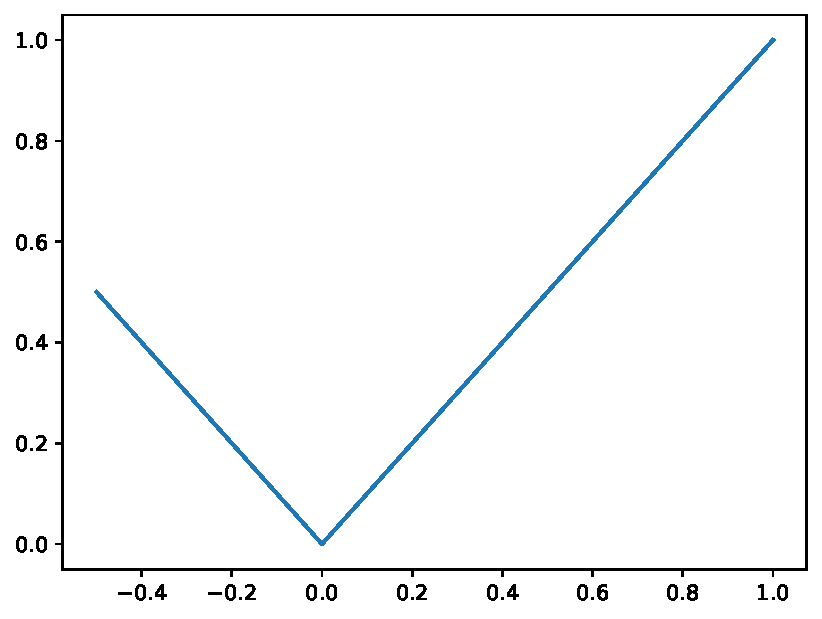
\includegraphics[width=0.8\textwidth]{./cap_ag/dados/fig_absx/fig}
    \caption{Gráfico referente ao Exemplo~\ref{cap_ag_sec_graf:ex:absx}.}
    \label{cap_ag_sec_graf:fig:absx}
  \end{figure}
  
\begin{lstlisting}
import matplotlib.pyplot as plt

# figure
fig = plt.figure()
# axes
ax = fig.add_subplot()
# plot
ax.plot([-0.5, 0, 1],
        [0.5, 0, 1])
# display
plt.show()
\end{lstlisting}

\end{ex}

No caso de curvas, podemos usamos um número adequado de pontos de forma que os segmentos de linhas ficam imperceptíveis a olho nu.

\begin{ex}\label{cap_ag_sec_graf:ex:fun}
  Consideramos a função
  \begin{equation}
    f(x) = \left\{
      \begin{array}{ll}
        -(x+1)^2-2 &, ~-2\leq x < -\frac{1}{2},\\
        |x| &, ~-\frac{1}{2}\leq x < 1,\\
        (x-2)^3 + 2, &, ~1\leq x < 3.
      \end{array}
    \right.
  \end{equation}
  A Figura~\ref{cap_ag_sec_graf:fig:fun}, mostra o gráfico de $f$ plotado com o código abaixo.

  \begin{figure}[H]
    \centering
    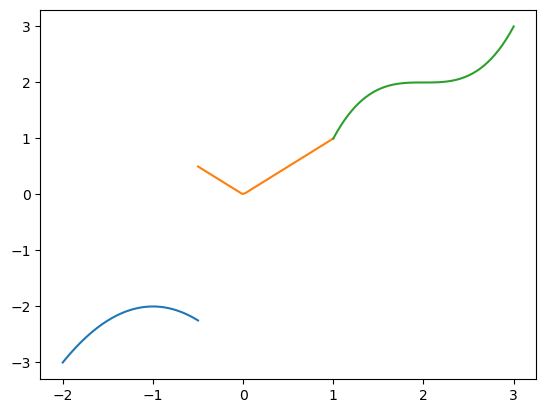
\includegraphics[width=0.8\textwidth]{./cap_ag/dados/fig_fun/fig}
    \caption{Gráfico referente ao Exemplo~\ref{cap_ag_sec_graf:ex:fun}.}
    \label{cap_ag_sec_graf:fig:fun}
  \end{figure}  

\begin{lstlisting}
import matplotlib as mpl
import matplotlib.pyplot as plt
import numpy as np

# figure
fig = plt.figure()
# axis
ax = fig.add_subplot()
# -2 <= x < -0.5
x = np.linspace(-2, -0.5)
ax.plot(x, -(x+1)**2-2)
# -0.5 <= x < 1
x = np.linspace(-0.5, 1)
ax.plot(x, np.fabs(x))
# 1 <= x < 3
x = np.linspace(1, 3)
ax.plot(x, (x-2)**3+2)
# display
plt.show()
\end{lstlisting}

\end{ex}

\subsection{Eixos}

No {\matplotlib}, os eixos\endnote{Não confundir com \lstinline+Axes+, um objeto que contém todos os elementos de um gráfico.} de um gráfico são objetos da classe \href{https://matplotlib.org/stable/api/axis_api.html\#matplotlib.axis.Axis}{\texttt{Axis}}\endnote{Consulte na \textit{web} \href{https://matplotlib.org/stable/api/axis_api.html\#matplotlib.axis.Axis}{Matplotlib: API Reference: matplotlib.axis.Axis}.}.

\begin{ex}\label{cap_ag_sec_graf:ex:axis}
  Com o código abaixo, produzimos a Figura~\ref{cap_ag_sec_graf:fig:eixos}, a qual contém o gráfico da função do Exemplo~\ref{cap_ag_sec_graf:fig:fun} com os eixos editados.

  \begin{figure}[H]
    \centering
    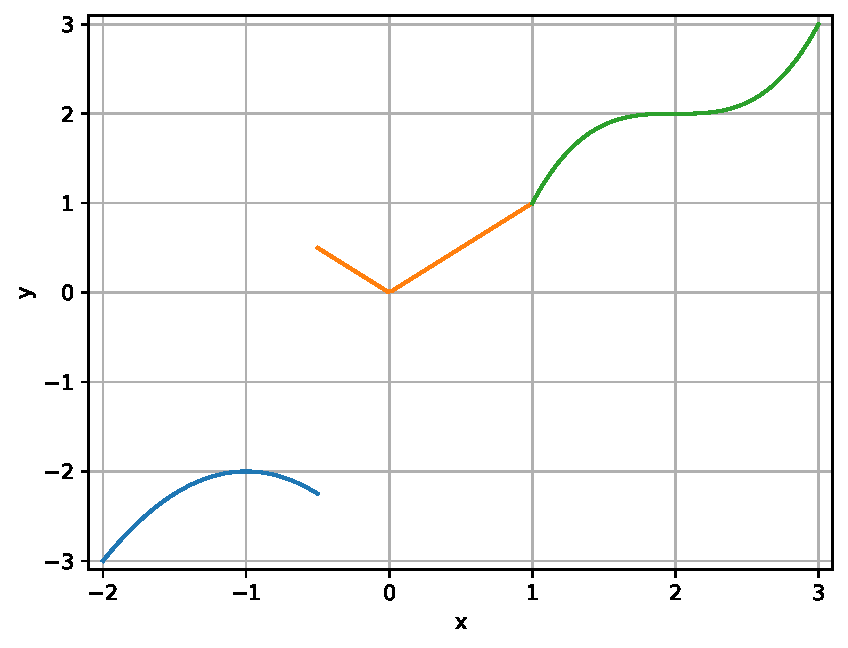
\includegraphics[width=0.8\textwidth]{./cap_ag/dados/fig_eixos/fig}
    \caption{Gráfico referente ao Exemplo~\ref{cap_ag_sec_graf:ex:axis}.}
    \label{cap_ag_sec_graf:fig:eixos}
  \end{figure}  

\begin{lstlisting}
import matplotlib as mpl
import matplotlib.pyplot as plt
import numpy as np

# figure
fig = plt.figure()
# axis
ax = fig.add_subplot()
# -2 <= x < -0.5
x = np.linspace(-2, -0.5)
ax.plot(x, -(x+1)**2-2)
# -0.5 <= x < 1
x = np.linspace(-0.5, 1)
ax.plot(x, np.fabs(x))
# 1 <= x < 3
x = np.linspace(1, 3)
ax.plot(x, (x-2)**3+2)
# eixo-x
ax.set_xlim((-2.1, 3.1))
ax.set_xticks([-2, -1, 0, 1, 2, 3])
ax.set_xlabel('x')
#eixo-y
ax.set_ylim((-3.1, 3.1))
ax.set_yticks([-3, -2, -1, 0, 1, 2, 3])
ax.set_ylabel('y')
# grid
ax.grid()
# display
plt.savefig('fig.png', bbox_inches='tight')
plt.savefig('fig.pdf', bbox_inches='tight')
plt.show()
\end{lstlisting}

\end{ex}

\subsection{Elementos Gráficos}

No {\matplotlib}, os elementos gráficos (basicamente tudo o que é visível, pontos, linhas, eixos, etc.) são objetos da classe \href{https://matplotlib.org/stable/api/artist_api.html\#artist-class}{\texttt{Artist}}\endnote{Consulte na \textit{web} \href{https://matplotlib.org/stable/api/artist_api.html\#artist-class}{Matplotlib: API Reference: matplotlib.artist}.}.

\begin{ex}\label{cap_ag_sec_graf:ex:elgraf}
  Com o código abaixo, produzimos a Figura~\ref{cap_ag_sec_graf:fig:elgraf}, a qual contém o gráfico da função do Exemplo~\ref{cap_ag_sec_graf:fig:elgraf} com os eixos editados.

  \begin{figure}[H]
    \centering
    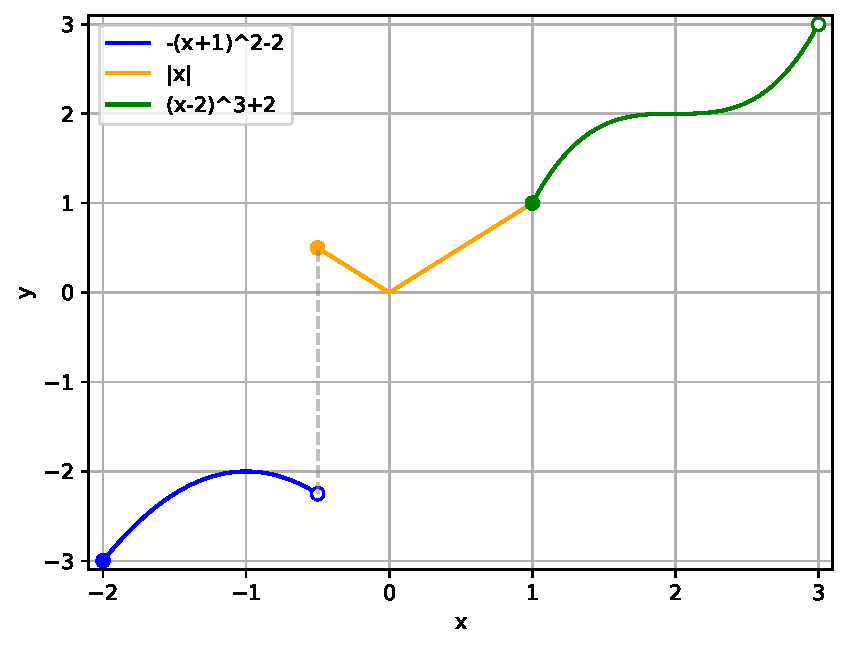
\includegraphics[width=0.8\textwidth]{./cap_ag/dados/fig_elgraf/fig}
    \caption{Gráfico referente ao Exemplo~\ref{cap_ag_sec_graf:ex:elgraf}.}
    \label{cap_ag_sec_graf:fig:elgraf}
  \end{figure}
  
\begin{lstlisting}
import matplotlib as mpl
import matplotlib.pyplot as plt
import numpy as np

# figure
fig = plt.figure()
# axis
ax = fig.add_subplot()

# -2 <= x < -0.5
x = np.linspace(-2, -0.5)
f1 = lambda x: -(x+1)**2-2
ax.plot(x, f1(x), color='blue',
        label='-(x+1)^2-2')
ax.plot([-2.], f1(-2.), linestyle='', marker='o',
        color='blue')
ax.plot([-0.5], f1(-0.5), ls='', marker='o',
        markerfacecolor='white', markeredgecolor='blue')

# -0.5 <= x < 1
x = np.linspace(-0.5, 1)
f2 = lambda x: np.fabs(x)
ax.plot(x, f2(x), color='orange', label='|x|')
ax.plot([-0.5], [f2(-0.5)], ls='', marker='o',
        color='orange')

ax.plot([-0.5, -0.5], [f1(-0.5), f2(-0.5)],
        ls = '--', color='gray', alpha=0.5)

# 1 <= x < 3
x = np.linspace(1, 3)
f3 = lambda x: (x-2)**3+2
ax.plot(x, f3(x), color='green',
        label='(x-2)^3+2')
ax.plot([1.], [f3(1.)], ls='', marker='o',
        color='green')
ax.plot([3.], [f3(3.)], ls='', marker='o',
        mfc='white', mec='green')

# eixo-x
ax.set_xlim((-2.1, 3.1))
ax.set_xticks([-2, -1, 0, 1, 2, 3])
ax.set_xlabel('x')
# eixo-y
ax.set_ylim((-3.1, 3.1))
ax.set_yticks([-3, -2, -1, 0, 1, 2, 3])
ax.set_ylabel('y')
# grid
ax.grid()
ax.legend()
# display
plt.savefig('fig.png', bbox_inches='tight')
plt.savefig('fig.pdf', bbox_inches='tight')
plt.show()
\end{lstlisting}

\end{ex}

\subsection{Textos e Anotações}

O comando \href{https://matplotlib.org/stable/api/_as_gen/matplotlib.axes.Axes.text.html\#matplotlib.axes.Axes.text}{\texttt{axes.text()}}\endnote{Consulte na \textit{web} \href{https://matplotlib.org/stable/api/_as_gen/matplotlib.axes.Axes.text.html\#matplotlib.axes.Axes.text}{Matplotlib: API Reference: matplotlib.axes.Axes.text}.} permite adicionar elementos \texttt{string} a um \lstinline+Axes+. Anotações, consistem em um apontamento, e podem ser adicionadas com o comando \href{https://matplotlib.org/stable/api/_as_gen/matplotlib.axes.Axes.annotate.html#matplotlib.axes.Axes.annotate}{\lstinline+axes.annotate()+}. Elementos texto suportam \LaTeX usando-se o marcador de texto \lstinline!$!.%$

\begin{ex}\label{cap_ag_sec_graf:ex:texto}
  Com o código abaixo, produzimos a Figura~\ref{cap_ag_sec_graf:fig:texto}, a qual contém o gráfico da função do Exemplo~\ref{cap_ag_sec_graf:fig:texto} com os eixos editados.

  \begin{figure}[H]
    \centering
    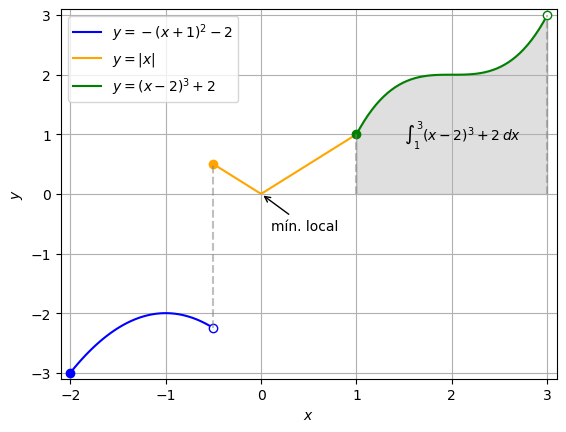
\includegraphics[width=0.8\textwidth]{./cap_ag/dados/fig_texto/fig}
    \caption{Gráfico referente ao Exemplo~\ref{cap_ag_sec_graf:ex:texto}.}
    \label{cap_ag_sec_graf:fig:texto}
  \end{figure}
  
\begin{lstlisting}
import matplotlib as mpl
import matplotlib.pyplot as plt
import numpy as np

# figure
fig = plt.figure()
# axis
ax = fig.add_subplot()

# -2 <= x < -0.5
x = np.linspace(-2, -0.5)
f1 = lambda x: -(x+1)**2-2
ax.plot(x, f1(x), color='blue',
        label='$y=-(x+1)^2-2$')
ax.plot([-2.], f1(-2.), linestyle='', marker='o',
        color='blue')
ax.plot([-0.5], f1(-0.5), ls='', marker='o',
        markerfacecolor='white', markeredgecolor='blue')

# -0.5 <= x < 1
x = np.linspace(-0.5, 1)
f2 = lambda x: np.fabs(x)
ax.plot(x, f2(x), color='orange', label='$y=|x|$')
ax.plot([-0.5], [f2(-0.5)], ls='', marker='o',
        color='orange')

ax.plot([-0.5, -0.5], [f1(-0.5), f2(-0.5)],
        ls = '--', color='gray', alpha=0.5)
# anotação
ax.annotate('mín. local', xy=(0,0), xytext=(0.1,-0.6),
            arrowprops={'arrowstyle':'->'})

# 1 <= x < 3
x = np.linspace(1, 3)
f3 = lambda x: (x-2)**3+2
ax.plot(x, f3(x), color='green',
        label='$y=(x-2)^3+2$')
ax.plot([1.], [f3(1.)], ls='', marker='o',
        color='green')
ax.plot([3.], [f3(3.)], ls='', marker='o',
        mfc='white', mec='green')

# hachurando
ax.fill_between(x, f3(x), color='gray', alpha=0.25)
ax.plot([1., 1.], [0., f3(1.)],
        ls='--', color='gray', alpha=0.5)
ax.plot([3., 3.], [0., f3(3.)],
        ls='--', color='gray', alpha=0.5)
# texto
ax.text(1.5, 0.9, '$\\int_{1}^3 (x-2)^3+2\,dx$')

# eixo-x
ax.set_xlim((-2.1, 3.1))
ax.set_xticks([-2, -1, 0, 1, 2, 3])
ax.set_xlabel('$x$')
# eixo-y
ax.set_ylim((-3.1, 3.1))
ax.set_yticks([-3, -2, -1, 0, 1, 2, 3])
ax.set_ylabel('$y$')
# grid
ax.grid()
ax.legend()
# display
plt.savefig('fig.png', bbox_inches='tight')
plt.savefig('fig.pdf', bbox_inches='tight')
plt.show()
\end{lstlisting}

\end{ex}

\subsection{Exercícios}

\begin{exer}
  Use o {\matplotlib} para produzir um gráfico para as seguintes funções:
  \begin{enumerate}[a)]
  \item $\displaystyle f(x) = x^2$, $-2 \leq x \leq 2$.
  \item $\displaystyle g(x) = 2x^3+2$, $-3 \leq x \leq 0$.
  \item $\displaystyle h(x) = \sen(x)$, $-\pi \leq x \leq \pi$.
  \end{enumerate}
\end{exer}

\begin{exer}
  Use o {\matplotlib} para plotar o gráfico da função sigmoid
  \begin{equation}
    f(x) = \frac{1}{1 + e^{-x}}.
  \end{equation}
  Na mesma área gráfica, plote retas tracejadas identificando suas assíntotas horizontais.
\end{exer}
\begin{resp}
  Dica: $y = 0$ e $y=1$ são assíntotas horizontais da função sigmoid.
\end{resp}

\begin{exer}
  Use o {\matplotlib} para plotar o gráfico de $f(x) = 1/x$, $-2 \leq x \leq 2$. Na mesma área gráfica, plote uma reta tracejada identificando a assíntota vertical de $f$.
\end{exer}
\begin{resp}
  Dica: $x = 0$ é assíntota vertical de $f$.
\end{resp}

\begin{exer}
  Use o {\matplotlib} para produzir um gráfico para a seguinte função definida por partes
  \begin{equation}
    f(x) = \left\{
      \begin{array}{ll}
        \cos(x) &, -\pi < x \leq 0,\\
        1-x^2 &, 0 < x \leq 2.
      \end{array}
    \right.
  \end{equation}
  Use de marcadores para identificar os pontos extremos de cada parte da função. Também, adicione o \textit{label} de cada eixo e uma legenda para identificar cada parte da função.
\end{exer}

\begin{exer}
  Em uma mesma área gráfica, plote as curvas $y = x + 1$ e $y = x^2$, e marque seus pontos de interseção. Para cada um destes pontos, inclua a anotação ``pto. de interseção''.
\end{exer}

\begin{exer}
  No gráfico da função sigmoid
  \begin{equation}
    f(x) = \frac{1}{1 + e^{-x}}
  \end{equation}
  hachure (pinte) a região que corresponde a área associada a integral definida
  \begin{equation}
    \int_1^3 f(x)\,dx.
  \end{equation}
\end{exer}
\begin{resp}
  Dica: use a função \href{https://matplotlib.org/stable/api/_as_gen/matplotlib.axes.Axes.fill_between.html\#matplotlib.axes.Axes.fill_between}{\texttt{Axes.fill\_between()}}\endnote{Consulte na \textit{web} \href{https://matplotlib.org/stable/api/_as_gen/matplotlib.axes.Axes.fill_between.html\#matplotlib.axes.Axes.fill_between}{Matplotlib: API Reference: matplotlib.axes.Axes.fill\_between}.}.
\end{resp}

\begin{ex}
  Em uma mesma área gráfica, plote a área entre as curvas $y = x + 1$ e $y = x^2$, $x=-1$ e $x=2$.
\end{ex}

\ifisbook
\subsubsection{Respostas}
\shipoutAnswer
\fi


% Este trabalho está licenciado sob a Licença Atribuição-CompartilhaIgual 4.0 Internacional Creative Commons. Para visualizar uma cópia desta licença, visite http://creativecommons.org/licenses/by-sa/4.0/deed.pt_BR ou mande uma carta para Creative Commons, PO Box 1866, Mountain View, CA 94042, USA.

\chapter{Orientação a Objetos}\label{cap_poo}

Programação Orientação a Objetos (POO) é um paradigma de programação baseado no conceito de classes de objetos. A classe define seus atributos (propriedades e métodos) de seus objetos. Todos os objetos de uma classe têm os mesmos atributos, mas são independentes um dos outros, sendo que cada um é uma instância própria da classe contendo seus próprios valores de seus atributos.

\section{Classe e Objeto}\label{cap_ob_sec_class}

\hl{Uma \emph{classe} é uma forma de estrutura que permite a alocação conjunta de dados e funções}. Em {\python}, a sintaxe de definição de uma classe é

\begin{lstlisting}
class NomeDaClasse:
    <bloco-0>
    <bloco-1>
    ...
    <bloco-2>
\end{lstlisting}

Usualmente, \hl{os blocos de programação consistem de definições de funções (métodos)}. Por exemplo,

\begin{lstlisting}
class MinhaClasse:
    def digaOla(self):
        print('Olá, Mundo!')

obj = MinhaClasse()
obj.digaOla()
\end{lstlisting}

Neste código, temos a definição da classe \lstinline+MinhaClasse+ (linhas 1-3). Esta classe contém o método \lstinline+MinhaClasse.digaOla()+ (linhas 2-3). Obrigatoriamente, \hl{na definição de um método de uma classe deve conter o primeiro parâmetro \texttt{self}}. Um objeto desta classe\endnote{Uma nova instância da classe.} e identificado por \lstinline+obj+ é alocado na linha 5. Na linha 6, este objeto chama seu método \lstinline+obj.digaOla()+.

O método especial \lstinline+__init__()+ é executado na construção de cada nova instância da classe (objeto da classe). Por exemplo,

\begin{lstlisting}
class Brasileira:
    pais = 'Brasil'
    def __init__(self, nome):
        self.nome = nome
        
    def digaOla(self):
        print('\nOlá!')
        print(f'Eu me chamo {self.nome}.')
        print(f'Sou do {self.pais}. :)')

x = Brasileira('Fulane')
x.digaOla()
y = Brasileira('Beltrane')
y.digaOla()
\end{lstlisting}

Aqui, o atributo \lstinline+Brasileira.pais+ é compartilhada entre todas as instâncias da classe (objetos), enquanto que \lstinline+Brasileira.nome+ é um atributo de cada objeto. O método \lstinline+__init()__+ (linhas 3-4) é executada no momento da criação de cada nova instância (linhas 11 e 13).

\begin{ex}\label{cap_oo_sec_class:ex:triangulo}
  No seguinte código, começamos a definição de uma classe para a manipulação de triângulos.

\begin{lstlisting}[caption=classTriangulo.py, label=cap_poo_sec_class:cod:classTriangulo]
import matplotlib.pyplot as plt

class Triangulo:
    '''
    Classe Triangulo ABC.
    '''
    num_lados = 3
    def __init__(self, A, B, C):
        # vértices
        self.A = A
        self.B = B
        self.C = C

    def plot(self):
        fig = plt.figure()
        ax = fig.add_subplot()
        # lados
        ax.plot([self.A[0], self.B[0]],
                [self.A[1], self.B[1]], marker='o', color='blue')
        ax.text((self.A[0]+self.B[0])/2,
                (self.A[1]+self.B[1])/2, 'c')
        ax.plot([self.B[0], self.C[0]],
                [self.B[1], self.C[1]], marker='o', color='blue')
        ax.text((self.B[0]+self.C[0])/2,
                (self.B[1]+self.C[1])/2, 'a')
        ax.plot([self.C[0], self.A[0]],
                [self.C[1], self.A[1]], marker='o', color='blue')
        ax.text((self.A[0]+self.C[0])/2,
                (self.A[1]+self.C[1])/2, 'b')
        # vertices
        ax.text(self.A[0], self.A[1], 'A')
        ax.text(self.B[0], self.B[1], 'B')
        ax.text(self.C[0], self.C[1], 'C')
        ax.grid()
        plt.show()

tria = Triangulo((0., 0.),
                 (2., 0.),
                 (1., 1.))
tria.plot()
\end{lstlisting}

\end{ex}

\subsection{Exercícios}

\begin{exer}
  Considere o Código~\ref{cap_poo_sec_class:cod:classTriangulo}. Adicione o método \lstinline+calcLados()+, que computa e aloca o comprimento de cada lado do triângulo.
\end{exer}
\begin{resp}

\begin{lstlisting}
import numpy as np
import matplotlib.pyplot as plt

class Triangulo:
    '''
    Classe Triangulo ABC.
    '''
    num_lados = 3
    def __init__(self, A, B, C):
        # vértices
        self.A = A
        self.B = B
        self.C = C
        # lados
        self.a = 0.
        self.b = 0.
        self.c = 0.

    def calcLados(self):
        self.a = np.sqrt((self.B[0]-self.C[0])**2\
                         + (self.B[1]-self.C[1])**2)
        self.b = np.sqrt((self.A[0]-self.C[0])**2\
                         + (self.A[1]-self.C[1])**2)
        self.c = np.sqrt((self.A[0]-self.B[0])**2\
                         + (self.A[1]-self.B[1])**2)
\end{lstlisting}

\end{resp}

\begin{exer}
  Considere o Código~\ref{cap_poo_sec_class:cod:classTriangulo}. Adicione o método \lstinline+calcPerimetro()+, que computa e retorna o valor do perímetro do triângulo.
\end{exer}
\begin{resp}

\begin{lstlisting}
import numpy as np
import matplotlib.pyplot as plt

class Triangulo:

    ...

    def perimetro(self):
        return self.a + self.b + self.c

    ...
\end{lstlisting}

\end{resp}

\begin{exer}
  Considere o Código~\ref{cap_poo_sec_class:cod:classTriangulo}. Adicione o método \lstinline+calcAngulos()+, que computa e aloca os ângulos do triângulo.
\end{exer}
\begin{resp}
  Dica: use a \href{https://pt.wikipedia.org/wiki/Lei_dos_cossenos}{Lei dos Cossenos}.
\end{resp}

\begin{exer}
  Considere o Código~\ref{cap_poo_sec_class:cod:classTriangulo}. Adicione o método \lstinline+area()+, que computa a área do triângulo.
\end{exer}
\begin{resp}
  Dica: use o \href{https://pt.wikipedia.org/wiki/Teorema_de_Her%C3%A3o}{Teorema de Herão}.
\end{resp}

\begin{exer}
  Similar a classe \lstinline+Triangulo+ (Código~\ref{cap_poo_sec_class:cod:classTriangulo}), implemente uma nova classe \lstinline+Quadrilateros+ com as seguintes propriedades e métodos de quadriláteros $ABCD$:
  \begin{enumerate}[a)]
  \item vértices (\lstinline+tuples+).
  \item lados (\lstinline+floats+).
  \item cálculo do perímetro (método).
  \item cálculo da área (método).
  \item visualização gráfica (método \textit+plot+).
  \end{enumerate}
\end{exer}

\begin{exer}
  Implemente uma classe para a manipulação de polinômios de segundo grau. A classe deve conter as seguintes propriedades e métodos:
  \begin{enumerate}[a)]
  \item coeficientes (\lstinline+floats+).
  \item cálculo do ponto de interseção com o eixo y (método).
  \item cálculo do vértice da parábola associada ao polinômio (método).
  \item cálculo das raízes do polinômio (método).
  \item plotagem do gráfico do polinômio (método).
  \end{enumerate}
\end{exer}
\begin{resp}
  Dica: utilize a notação $p(x) = ax^2 + bx + c$.
\end{resp}

\ifisbook
\subsubsection{Respostas}
\shipoutAnswer
\fi

  

\section{Herança}\label{cap_oo_sec_her}

\hl{Na programação orientada-a-objetos, \emph{herança} consiste na definição de uma classe derivada a partir de uma dada classe base}. A sintaxe de definição de uma classe derivada é

\begin{lstlisting}
class ClasseDerivada(ClasseBase):
    bloco-0
    bloco-1
    ...
    bloco-n
\end{lstlisting}

\hl{A classe derivada herda todos os atributos da classe base}. Por exemplo, consideramos o seguinte código

\begin{lstlisting}
class ClasseBase:
    def __init__(self, nome):
        self.nome = nome
        
    def digaOi(self):
        print(f'{self.nome}: Oi!')

class ClasseDerivada(ClasseBase):
    def digaTchau(self):
        print(f'{self.nome}: Tchau!')

obj = ClasseDerivada('Fulane')
obj.digaOi()
obj.digaTchau()
\end{lstlisting}

Nas linhas 1-6, a classe base é definida contendo dois métodos: \lstinline+self.__init__()+ chamado na criação de um objeto da classe (uma instância) e, \lstinline+self.digaOi()+ que imprime uma saudação. A classe derivada é definida nas linhas 8-10, ela herda os atributos da classe base e contém um novo método \lstinline+self.digaTchau()+, que imprime uma mensagem de despedida.

A criação de uma instância (objeto) de uma classe derivada é feita da mesma forma que de uma classe base. \hl{A referência a um atributo do objeto é, primeiramente, buscada na classe derivada e, se não encontrada, é buscada na classe base}. Este regra aplica-se recursivamente se a classe base também é derivada de outra classe. \hl{Isso permite que uma classe derivada sobreponha atributos de sua classe base}.

\begin{obs}\normalfont{(\hl{\texttt{super()}}.)}
O método \href{https://docs.python.org/3/library/functions.html\#super}{\lstinline+super()+}\endnote{Consulte na \textit{web} \href{https://docs.python.org/3/library/functions.html\#super}{ The Python Standard Library: Built-in Functions: super}.} retorno um objeto \textit{proxy} da classe base, que acessa os atributos desta classe.
\end{obs}

\begin{ex}
  Vamos criar uma classe para manipular triângulo isósceles. Para tanto, vamos derivá-la a partir da classe \lstinline+Triangulo+ definida no Exemplo~\ref{cap_oo_sec_class:ex:triangulo}. Vamos assumir que os triângulos isósceles têm vértices $\Delta ABC$ com lados $b = AC$ e $a = BC$ de mesmo tamanho.

\begin{lstlisting}[caption=classTrianguloIsosceles.py, label=cap_oo_sec_her:cod:classTrianguloIsosceles]
import numpy as np
import matplotlib.pyplot as plt

class Triangulo:
    '''
    Classe Triangulo ABC.
    '''
    num_lados = 3
    def __init__(self, A, B, C):
        # vértices
        self.A = A
        self.B = B
        self.C = C

    def plot(self):
        fig = plt.figure()
        ax = fig.add_subplot()
        # lados
        ax.plot([self.A[0], self.B[0]],
                [self.A[1], self.B[1]], marker='o', color='blue')
        ax.text((self.A[0]+self.B[0])/2,
                (self.A[1]+self.B[1])/2, 'c')
        ax.plot([self.B[0], self.C[0]],
                [self.B[1], self.C[1]], marker='o', color='blue')
        ax.text((self.B[0]+self.C[0])/2,
                (self.B[1]+self.C[1])/2, 'a')
        ax.plot([self.C[0], self.A[0]],
                [self.C[1], self.A[1]], marker='o', color='blue')
        ax.text((self.A[0]+self.C[0])/2,
                (self.A[1]+self.C[1])/2, 'b')
        # vertices
        ax.text(self.A[0], self.A[1], 'A')
        ax.text(self.B[0], self.B[1], 'B')
        ax.text(self.C[0], self.C[1], 'C')
        ax.grid()
        plt.show()


class TrianguloIsosceles(Triangulo):
    def __init__(self,A,B,C):
        # vertices
        super().__init__(A,B,C)
        # lados
        self.a = self.b = self.c = 0.

    def calcLados(self):
        self.a = np.sqrt((self.B[0] - self.C[0])**2\
                         + (self.B[1] - self.C[1])**2)
        self.b = np.sqrt((self.A[0] - self.C[0])**2\
                         + (self.A[1] - self.C[1])**2)
        self.c = np.sqrt((self.B[0] - self.A[0])**2\
                         + (self.B[1] - self.A[1])**2)
        assert(self.a == self.b)

tria = TrianguloIsosceles((1,0),
                          (3,0),
                          (2,1))
tria.plot()
tria.calcLados()
\end{lstlisting}

\end{ex}

\begin{obs}\normalfont{(\hl{Herança Múltipla}.)}
  {\python} suporta a herança múltipla de classes. A sintaxe é

\begin{lstlisting}
class ClasseDerivada(Base1, Base2, ..., BraseN):
    bloco-0
    bloco-1
    ...
    bloco-m
\end{lstlisting}
  
Quando um objeto da classe derivada faz uma referência a um atributo, este é procurado de forma sequencial (e recursiva, caso uma das classe bases seja também uma classe derivada) começando por essa e, caso não encontrado, buscando-se nas classes \lstinline+Base1+, \lstinline+Base2+, ..., \lstinline+BaseN+.
\end{obs}

\subsection{Exercícios}

\begin{exer}
  No Código~\ref{cap_oo_sec_her:cod:classTrianguloIsosceles}, adicione à classe \lstinline+Triangulo+ o método \lstinline+Triangulo.perimetro()+ que computa, aloca e retorna o valor do perímetro do triângulo. Então, sobreponha o método à classe \lstinline+TrianguloIsosceles+. Teste seu código para diferentes triângulos.
\end{exer}
\begin{resp}

\begin{lstlisting}
class Triangulo:
    def __init(self,A,B,C)__:
        ...
        self.p = 0.
        ...
    ...
    def perimetro(self):
        self.p = self.a\
               + self.b\
               + self.c
        return self.p
    ...

class TrianguloIsosceles(Triangulo):
    ...
    def perimetro(self):
        self.p = 2*self.a + self.c
        return self.p
    ...
\end{lstlisting}

\end{resp}

\begin{exer}\label{cap_oo_sec_her:exer:retangulo}
  Implemente uma classe \lstinline+Retangulo(largura, altura)+ para a manipulação de retângulos de \lstinline+largura+ e \lstinline+altura+ dadas. Equipe sua classe com métodos para o cálculo do perímetro, da diagonal e da área de retângulo. Então, implemente a classe derivada \lstinline+Quadrado(lado)+ para a manipulação de quadrados de \lstinline+lado+ dado. Teste sua implementação para diferentes retângulos e quadrados.
\end{exer}
\begin{resp}

\begin{lstlisting}
import math as m

class Retangulo:
    def __init__(self, largura, altura):
        self.largura = largura
        self.altura = altura

    def perimetro(self):
        return self.largura\
               + self.altura

    def diagonal(self):
        return m.sqrt(self.largura**2\
                      + self.altura**2)

    def area(self):
        return self.largura\
               * self.altura

class Quadrado(Retangulo):
    def __init__(self,lado):
        super().__init__(lado,lado)
\end{lstlisting}

\end{resp}

\begin{exer}
  Refaça o Exercício~\ref{cap_oo_sec_her:exer:retangulo} sobrepondo os métodos do cálculo do perímetro, da diagonal e da área para quadrados.
\end{exer}
\begin{resp}
  Dica: para um quadrado de lado $l$, o perímetro é $p = 2l$, por exemplo.
\end{resp}

\begin{exer}
  Implemente uma classe \lstinline+TrianguloEquilatero+, derivada da classe \lstinline+TrianguloIsosceles+ definida no Código~\ref{cap_oo_sec_her:cod:classTrianguloIsosceles}. Adicione métodos para o cálculo do perímetro e da altura de triângulo equiláteros. Teste seu código para diferentes triângulos.
\end{exer}
\begin{resp}
  Dica:

\begin{lstlisting}
...
class Triangulo:
   def __init__(self,A,B,C):
      ...
   ...

class TrianguloIsosceles(Triangulo):
   ...

class TrianguloEquilatero(TrianguloIsosceles):
   def __init__(self,A,B,C):
      super().__init__(A,B,C)

   def perimetro(self):
      ...

   def altura(self):
      ...
   
   def area(self):
      ...
\end{lstlisting}

\end{resp}

\begin{exer}
  Implemente:
  \begin{enumerate}[a)]
  \item Uma classe \lstinline+Quadrilatero+ para a manipulação de quadriláteros de lados $abcd$. Equipe sua classe com um método \lstinline+self.perimetro()+ para o cálculo do perímetro.
  \item Uma classe \lstinline+Retangulo+, derivada da classe \lstinline+Quadrilatero+, para a manipulação de retângulos de lado dado e altura dada. Na classe derivada, sobreponha o método \lstinline+self.perimetro()+ para o cálculo do perímetro e implemente novos métodos para o cálculo da diagonal e da área de retângulos.
  \item Uma classe \lstinline+Quadrado+, derivada da classe \lstinline+Retangulo+, para a manipulação de quadrados de lado dado. Na classe derivada, sobreponha os métodos para os cálculos do perímetro, da diagonal e da área.
  \end{enumerate}
\end{exer}

\ifisbook
\subsubsection{Respostas}
\shipoutAnswer
\fi


% endnotes
\clearpage
\phantomsection
\addcontentsline{toc}{chapter}{Notas}
\theendnotes

%references
\ifisbook
\clearpage
\phantomsection
\addcontentsline{toc}{chapter}{\bibname}
\fi

\begin{thebibliography}{99}
\bibitem{Banin2021a}
  Banin, S.L.. Python 3 - Conceitos e Aplicações - Uma Abordagem Didática, Saraiva: São Paulo, 2021. ISBN: \texttt{978-8536530253}.

\bibitem{Cormen2021a}
  Cormen, T.. Desmitificando Algoritmos, Grupo GEN: São Paulo, 2021. ISBN: \texttt{978-8595153929}.

\bibitem{Cormen2012a}
  Cormen, T.. Algoritmos - Teoria e Prática, Grupo GEN: São Paulo, 2012. ISBN: \texttt{978-8595158092}.

\bibitem{Grus2021a}
  Grus, J.. Data Science do Zero, Alta Books: Rio de Janeiro, 2021. ISBN: \texttt{978-8550816463}.

\bibitem{Matplotlib2024a}
  Hunter, J.; Dale, D.; Firing, E.; Droettboom, M. \& Matplotlib development team. NumPy documentation, versão 3.8.3, disponível em \url{https://matplotlib.org/stable/}.

\bibitem{NumPy2024a}
  NumpPy Developers. NumPy documentation, versão 1.26, disponível em \url{https://numpy.org/doc/stable/}.

\bibitem{Python2024a}
  Python Software Foundation. Python documentation, versão 3.12.2, disponível em \url{https://docs.python.org/3/}.

\bibitem{Ribeiro2021a}
  Ribeiro, J.A.. Introdução à Programação e aos Algoritmos, LTC: São Paulo, 2021. ISBN: \texttt{978-8521636410}.

\bibitem{Wazlawick2021a}
  Wazlawick, R.. Introdução a Algoritmos e Programação com Python - Uma Abordagem Dirigida por Testes, Grupo GEN: São Paulo, 2021. ISBN \texttt{978-8595156968}.

\end{thebibliography}

% index
\ifisbook
\printindex
\fi

\end{document}
